
\documentclass[12pt, a4paper]{report}

\usepackage{epsfig}
\usepackage{subfigure}
%\usepackage{amscd}
\usepackage{amssymb}
\usepackage{graphicx}
%\usepackage{amscd}
\usepackage{amssymb}
\usepackage{subfiles}
\usepackage{framed}
\usepackage{subfiles}
\usepackage{amsthm, amsmath}
\usepackage{amsbsy}
\usepackage{framed}
\usepackage[usenames]{color}
\usepackage{listings}
\lstset{% general command to set parameter(s)
	basicstyle=\small, % print whole listing small
	keywordstyle=\color{red}\itshape,
	% underlined bold black keywords
	commentstyle=\color{blue}, % white comments
	stringstyle=\ttfamily, % typewriter type for strings
	showstringspaces=false,
	numbers=left, numberstyle=\tiny, stepnumber=1, numbersep=5pt, %
	frame=shadowbox,
	rulesepcolor=\color{black},
	,columns=fullflexible
} %
%\usepackage[dvips]{graphicx}
\usepackage{natbib}
\bibliographystyle{chicago}
\usepackage{vmargin}
% left top textwidth textheight headheight
% headsep footheight footskip
\setmargins{1.0cm}{0.75cm}{18.5 cm}{22cm}{0.5cm}{0cm}{1cm}{1cm}
%\voffset=-2.5cm
%\oddsidemargin=1cm
%\textwidth = 520pt

\renewcommand{\baselinestretch}{1.5}
\pagenumbering{arabic}
\theoremstyle{plain}
\newtheorem{theorem}{Theorem}[section]
\newtheorem{corollary}[theorem]{Corollary}
\newtheorem{ill}[theorem]{Example}
\newtheorem{lemma}[theorem]{Lemma}
\newtheorem{proposition}[theorem]{Proposition}
\newtheorem{conjecture}[theorem]{Conjecture}
\newtheorem{axiom}{Axiom}
\theoremstyle{definition}
\newtheorem{definition}{Definition}[section]
\newtheorem{notation}{Notation}
\theoremstyle{remark}
\newtheorem{remark}{Remark}[section]
\newtheorem{example}{Example}[section]
\renewcommand{\thenotation}{}
\renewcommand{\thetable}{\thesection.\arabic{table}}
\renewcommand{\thefigure}{\thesection.\arabic{figure}}
\title{Research notes: linear mixed effects models}
\author{ } \date{ }


\begin{document}
	\author{Kevin O'Brien}
	\title{Mixed Models for Method Comparison Studies}
	\tableofcontents
	\chapter{Review of MCS Methodologies}
	\section{Bland-Altman methodology}
	The issue of whether two measurement methods comparable to the 	extent that they can be used interchangeably with sufficient
	accuracy is encountered frequently in scientific research.
	Historically comparison of two methods of measurement was carried 	out by use of paired sample $t-$test, correlation coefficients or
	simple linear regression. Simple linear regression is unsuitable for method comparison studies because of the required assumption that one variable is measured without error. In comparing two methods, both methods are assume to have attendant random error.
	
	Statisticians Martin Bland and Douglas Altman recognized the inadequacies of these analyzes and
	articulated quite thoroughly the basis on which of which they are unsuitable for comparing two methods of measurement \citep*{BA83}. Furthermore they proposed their simple methodology specifically constructed for method comparison studies. They acknowledge the opportunity to apply other valid, but complex, methodologies, but argue that a simple approach is preferable, especially when the
	results must be `explained to non-statisticians'.
	
	Notwithstanding previous remarks about linear regression, the first step recommended, which the authors argue should be mandatory, is construction of a simple scatter plot of the data. The line of equality should also be shown, as it is necessary to give the correct interpretation of how both methods compare. In the case of good agreement, the observations would be distributed closely along the line of equality. A scatter plot of the Grubbs data is shown in Figure 1.1. Visual inspection confirms the previous conclusion that there is an inter-method bias present, i.e. Fotobalk device has a tendency to record a lower velocity.
	
	\begin{figure}[h!]
		\begin{center}
			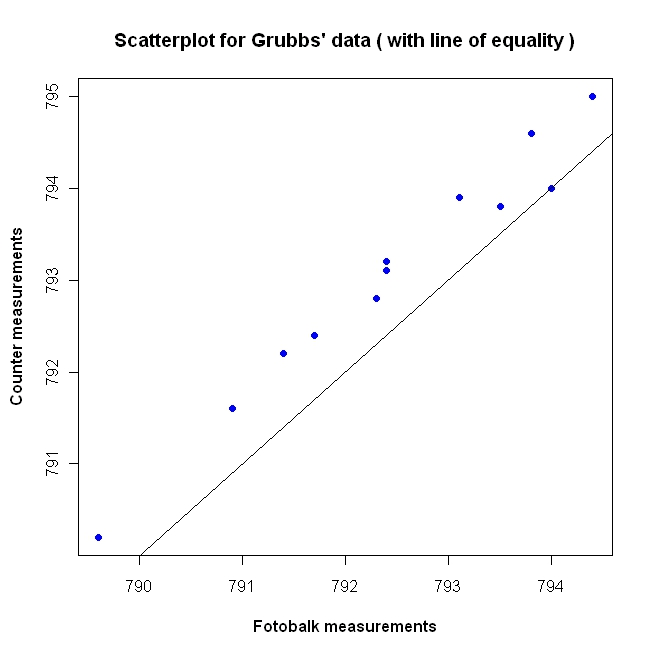
\includegraphics[width=100mm]{images/GrubbsScatter.jpeg}
			\caption{Scatter plot For Fotobalk and Counter Methods.}\label{GrubbsScatter}
		\end{center}
	\end{figure}
	
	\citet{Dewitte} notes that scatter plots were very seldom presented in the Annals of Clinical Biochemistry. This apparently
	results from the fact that the `Instructions for Authors' dissuade the use of regression analysis, which conventionally is accompanied by a scatter plot.
	
	\newpage
	\subsection{Bland-Altman plots}
	
	In light of shortcomings associated with scatterplots, \citet*{BA83} recommend a further analysis of the data. Firstly
	case-wise differences of measurements of two methods $d_{i} = y_{1i}-y_{2i} \mbox{ for }i=1,2,\dots,n$ on the same subject
	should be calculated, and then the average of those measurements ($a_{i} = (y_{1i} + y_{2i})/2 \mbox{ for }i=1,2,\dots, n$).
	
	\citet{BA83} proposes a scatterplot of the case-wise averages and differences of two methods of measurement. This scatterplot has since become widely known as the Bland-Altman plot. \citet*{BA83} express the
	motivation for this plot thusly:
	\begin{quote}
		``From this type of plot it is much easier to assess the magnitude
		of disagreement (both error and bias), spot outliers, and see
		whether there is any trend, for example an increase in (difference) for high values. This way of plotting the data is a very powerful way of displaying the results of a method comparison study."
	\end{quote}
	
	The case wise-averages capture several aspects of the data, such as expressing the range over which the values were taken, and assessing whether the assumptions of constant variance holds.
	Case-wise averages also allow the case-wise differences to be presented on a two-dimensional plot, with better data visualization qualities than a one dimensional plot. \citet{BA86}
	cautions that it would be the difference against either measurement value instead of their average, as the difference relates to both value. This methodology has proved very popular, and the Bland-Altman plots is widely regarded as powerful graphical methodology for making a visual assessment of the data.
	
	The magnitude of the inter-method bias between the two methods is simply the average of the differences $\bar{d}$. This inter-method bias is represented with a line on the Bland-Altman plot. As the objective of the Bland-Altman plot is to advise on the agreement of two methods, it is the case-wise differences that are also particularly relevant. The variances around this bias is estimated by the standard deviation of these differences $S_{d}$.
	
	\subsection{Bland-Altman plots for the Grubbs data}
	
	In the case of the Grubbs data the inter-method bias is $-0.61$ metres per second, and is indicated by the dashed line on Figure 1.2. By inspection of the plot, it is also possible to compare the precision of each method. Noticeably the differences tend to increase as the averages increase.
	
	
	The Bland-Altman plot for comparing the `Fotobalk' and `Counter'
	methods, which shall henceforth be referred to as the `F vs C' comparison,  is depicted in Figure 1.2, using data from Table 1.3.
	The presence and magnitude of the inter-method bias is indicated
	by the dashed line.
	\newpage
	
	%Later it will be shown that case-wise differences are the sole
	%component of the next part of the methodology, the limits of
	%agreement.
	
	
	\begin{table}[h!]
		\renewcommand\arraystretch{0.7}%
		\begin{center}
			\begin{tabular}{|c||c|c||c|c|}
				\hline
				Round & Fotobalk  & Counter  & Differences  & Averages  \\
				&  [F] & [C] & [F-C] &  [(F+C)/2] \\
				\hline
				1 & 793.8 & 794.6 & -0.8 & 794.2 \\
				2 & 793.1 & 793.9 & -0.8 & 793.5 \\
				3 & 792.4 & 793.2 & -0.8 & 792.8 \\
				4 & 794.0 & 794.0 & 0.0 & 794.0 \\
				5 & 791.4 & 792.2 & -0.8 & 791.8 \\
				6 & 792.4 & 793.1 & -0.7 & 792.8 \\
				7 & 791.7 & 792.4 & -0.7 & 792.0 \\
				8 & 792.3 & 792.8 & -0.5 & 792.5 \\
				9 & 789.6 & 790.2 & -0.6 & 789.9 \\
				10 & 794.4 & 795.0 & -0.6 & 794.7 \\
				11 & 790.9 & 791.6 & -0.7 & 791.2 \\
				12 & 793.5 & 793.8 & -0.3 & 793.6 \\
				\hline
			\end{tabular}
			\caption{Fotobalk and Counter methods: differences and averages.}
		\end{center}
	\end{table}
	
	\begin{table}[h!]
		\renewcommand\arraystretch{0.7}%
		\begin{center}
			\begin{tabular}{|c||c|c||c|c|}
				\hline
				Round & Fotobalk  & Terma  & Differences  & Averages  \\
				&  [F] & [T] & [F-T] &  [(F+T)/2] \\
				\hline
				1 & 793.8 & 793.2 & 0.6 & 793.5 \\
				2 & 793.1 & 793.3 & -0.2 & 793.2 \\
				3 & 792.4 & 792.6 & -0.2 & 792.5 \\
				4 & 794.0 & 793.8 & 0.2 & 793.9 \\
				5 & 791.4 & 791.6 & -0.2 & 791.5 \\
				6 & 792.4& 791.6 & 0.8 & 792.0 \\
				7 & 791.7 & 791.6 & 0.1 & 791.6 \\
				8 & 792.3 & 792.4 & -0.1 & 792.3 \\
				9 & 789.6 & 788.5 & 1.1 & 789.0 \\
				10 & 794.4 & 794.7 & -0.3 & 794.5 \\
				11 & 790.9 & 791.3 & -0.4 & 791.1 \\
				12 & 793.5 & 793.5 & 0.0 & 793.5 \\
				
				\hline
			\end{tabular}
			\caption{Fotobalk and Terma methods: differences and averages.}
		\end{center}
	\end{table}
	
	\newpage
	
	\begin{figure}[h!]
		\begin{center}
			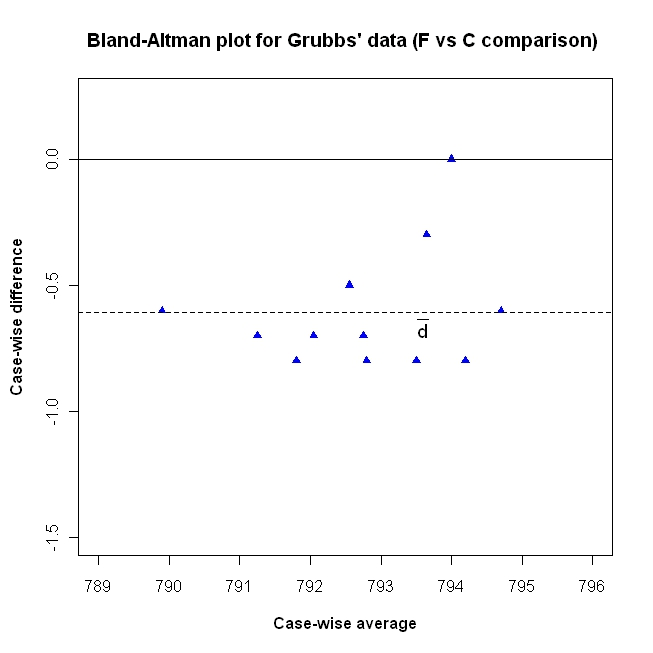
\includegraphics[width=120mm]{images/GrubbsBAplot-noLOA.jpeg}
			\caption{Bland-Altman plot For Fotobalk and Counter methods.}\label{GrubbsBA-noLOA}
		\end{center}
	\end{figure}
	
	
	
	In Figure 1.3 Bland-Altman plots for the `F vs C' and `F vs T'
	comparisons are shown, where `F vs T' refers to the comparison of
	the `Fotobalk' and `Terma' methods. Usage of the Bland-Altman plot
	can be demonstrate in the contrast between these comparisons. By inspection, there exists a larger inter-method bias in the `F vs C' comparison than in the `F vs T' comparison. Conversely there
	appears to be less precision in `F vs T' comparison, as indicated
	by the greater dispersion of covariates.
	
	\begin{figure}[h!]
		\begin{center}
			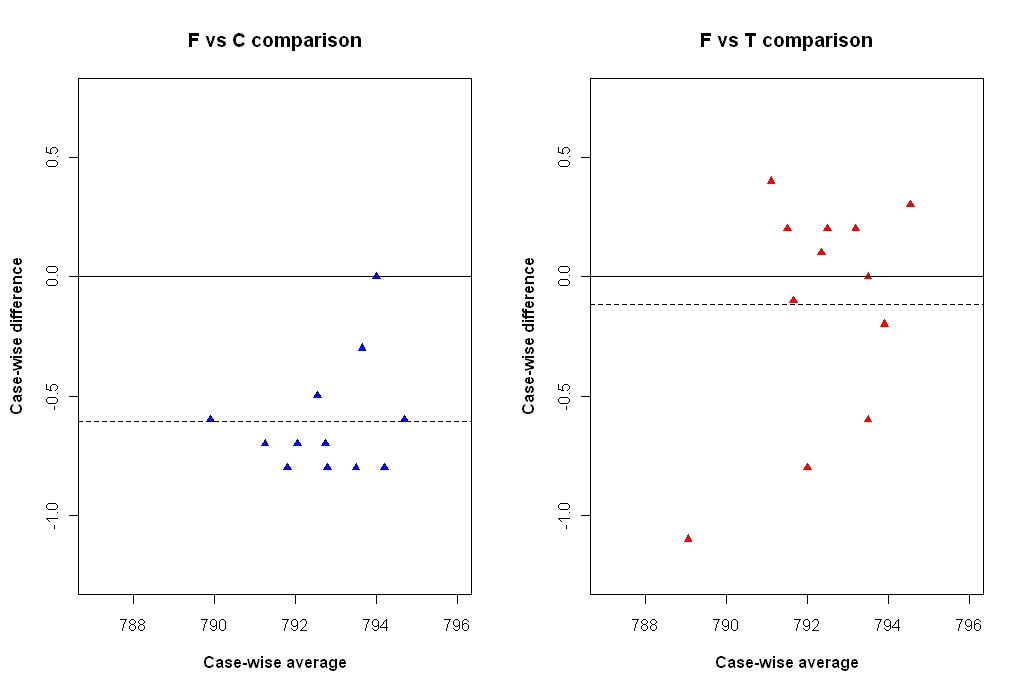
\includegraphics[height=90mm]{images/GrubbsDataTwoBAplots.jpeg}
			\caption{Bland-Altman plots for Grubbs' F vs C and F vs T comparisons.}\label{GrubbsDataTwoBAplots}
		\end{center}
	\end{figure}
	
	\newpage
	
	
	\subsection{Adverse features}
	
	Estimates for inter-method bias and variance of differences are only meaningful if there is uniform inter-bias and variability throughout the range of measurements. Fulfilment of these assumptions can be checked by visual inspection of the plot.The prototype Bland-Altman plots depicted in Figures 1.4, 1.5 and 1.6 are derived from simulated data, for the purpose of demonstrating how the plot would inform an analyst of features that would adversely affect use of the recommended methodology.
	
	Figure 1.4 demonstrates how the Bland-Altman plot would indicate
	increasing variance of differences over the measurement range.
	Fitted regression lines, for both the upper and lower half of the
	plot, has been added to indicate the trend. Figure 1.5 is an
	example of cases where the inter-method bias changes over the
	measurement range. This is known as proportional bias, and is
	defined by \citet{ludbrook97} as meaning that `one method gives values that are higher (or lower) than those from the other by an 	amount that is proportional to the level of the measured variable'. In both Figures 1.4 and 1.5, the assumptions necessary
	for further analysis using the limits of agreement are violated.
	
	Application of regression techniques to the Bland-Altman plot, and
	subsequent formal testing for the constant variability of
	differences is informative. The data set may be divided into two
	subsets, containing the observations wherein the difference values
	are less than and greater than the inter-method bias respectively.
	For both of these fits, hypothesis tests for the respective slopes
	can be performed. While both tests can be considered separately,
	multiple comparison procedures, such as the Benjamini-Hochberg
	\citep{BH} test, should be also be used.
	
	\begin{figure}[h!]
		\begin{center}
			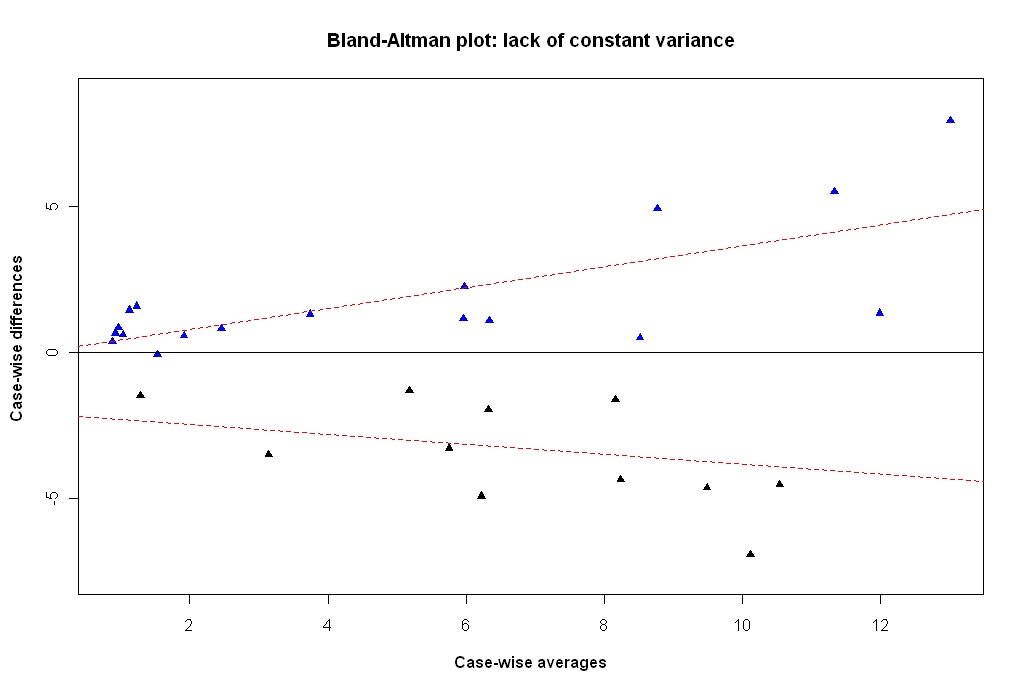
\includegraphics[height=90mm]{images/BAFanEffect.jpeg}
			\caption{Bland-Altman plot demonstrating the increase of variance over the range.}\label{BAFanEffect}
		\end{center}
	\end{figure}
	
	\begin{figure}[h!]
		\begin{center}
			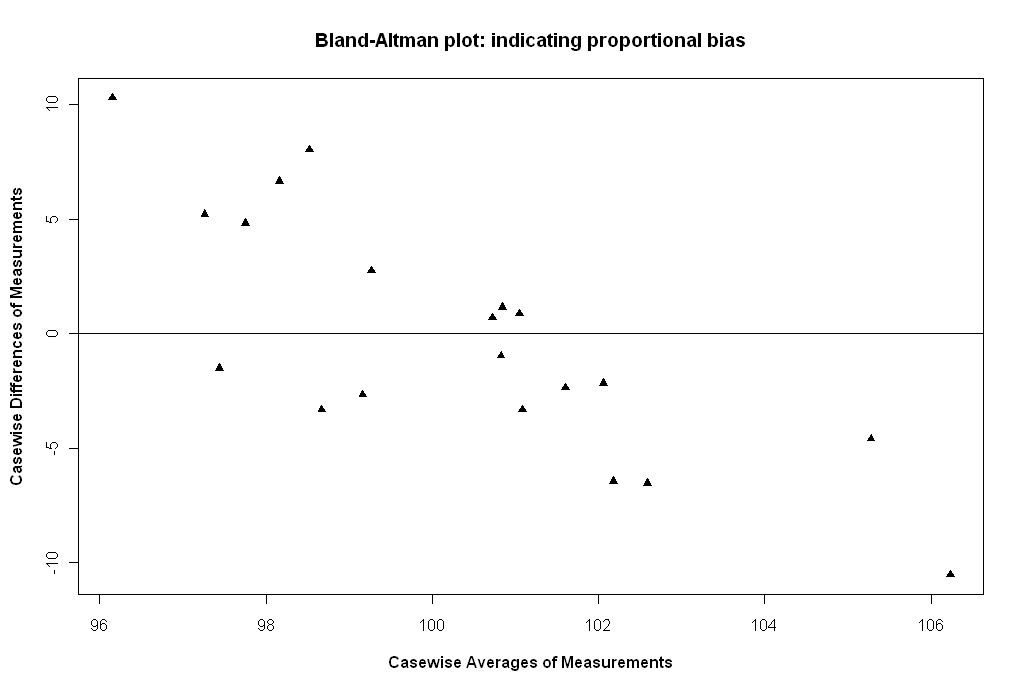
\includegraphics[height=90mm]{images/PropBias.jpeg}
			\caption{Bland-Altman plot indicating the presence of proportional bias.}\label{PropBias}
		\end{center}
	\end{figure}
	
	
	
	
	
	
	\subsection{Replicate Measurements}
	
	Thus far, the formulation for comparison of two measurement methods is one where one measurement by each method is taken on	each subject. Should there be two or more measurements by each methods, these measurement are known as `replicate measurements'.
	\citet{BXC2008} recommends the use of replicate measurements, but acknowledges the additional computational complexity.
	
	\citet*{BA86} address this problem by offering two different approaches. The premise of the first approach is that replicate
	measurements can be treated as independent measurements. The second approach is based upon using the mean of the each group of
	replicates as a representative value of that group. Using either
	of these approaches will allow an analyst to estimate the inter
	method bias.
	
	%\subsubsection{Mean of Replicates Limits of Agreement}
	
	However, because of the removal of the effects of the replicate
	measurements error, this would cause the estimation of the
	standard deviation of the differences to be unduly small.
	\citet*{BA86} propose a correction for this.
	
	\citet{BXC2008} takes issue with the limits of agreement based on
	mean values of replicate measurements, in that they can only be interpreted as prediction
	limits for difference between means of repeated measurements by
	both methods, as opposed to the difference of all measurements.
	Incorrect conclusions would be caused by such a misinterpretation.
	\citet{BXC2008} demonstrates how the limits of agreement
	calculated using the mean of replicates are `much too narrow as
	prediction limits for differences between future single
	measurements'. This paper also comments that, while treating the
	replicate measurements as independent will cause a downward bias
	on the limits of agreement calculation, this method is preferable
	to the `mean of replicates' approach.
	
	
	
	\subsection{Identifiability}
	\citet{DunnSEME} highlights an important issue regarding using
	models such as these, the identifiability problem. This comes as a result of there being too many parameters to be estimated.
	Therefore assumptions about some parameters, or estimators used,
	must be made so that others can be estimated. For example in literature the variance
	ratio $\lambda=\frac{\sigma^{2}_{1}}{\sigma^{2}_{2}}$
	must often be assumed to be equal to $1$ \citep{linnet98}.\citet{DunnSEME} considers methodologies based on two methods with single measurements on each subject as inadequate for a serious
	study on the measurement characteristics of the methods. This is
	because there would not be enough data to allow for a meaningful
	analysis. There is, however, a contrary argument that in many
	practical settings it is very difficult to get replicate
	observations when the measurement method requires invasive medical
	procedure.
	
	
	
	
	\chapter{Introduction to Method Comparison Studies}
	\begin{abstract}
		The first chapter will consider the topic of Method Comparison Studies, and discuss the impact of the Bland-Altman Methodology. A detailed discussion of the Bland-Altman Methodology will be covered in chapter two.
	\end{abstract}
	
	
	\section{Introductory Definitions}
	
	
	
	
	The problem of assessing the agreement between two or more methods of measurement is ubiquitous in scientific research, and is commonly referred to as a `method comparison study'. Published examples of method comparison studies can be found in disciplines
	as diverse as Pharmacology \citep{ludbrook97}, Anaesthesia \citep{Myles}, and cardiac imaging methods \citep{Krumm}.
	\smallskip
	Method Comparison Studies is a branch of statistics used to compare the results of two different method of measurement, measuring the same subject samples. Consider a set of n samples. Measurements are taken on each of the n samples using both methods. This will enable comparison of the method used.
	\smallskip
	In many cases the purpose of the study is to calibrate a new method of measurement against a ‘Gold Standard’ method. A ‘Gold Standard’ method is the known method that is considered most precise in its measurement. It should not be assumed that there is no error present in its measurements.
	\smallskip
	The Gold Standard may not be financially feasible for general use, and therefore more economical methods, of suitable levels of precisions, must be devised. Method Comparison studies is used to ascertain the levels of precision of such methods.
	\smallskip
	
	To illustrate the characteristics of a typical method comparison study consider the data in Table I, taken from \citet{Grubbs73}.
	\smallskip
	In each of twelve experimental trials a single round of ammunition was fired from a 155mm gun, and its velocity was measured
	simultaneously (and independently) by three chronographs devices, referred to here as `Fotobalk', `Counter' and `Terma'.
	\smallskip
	
	
	\newpage
	
	\begin{table}[ht]
		\begin{center}
			\begin{tabular}{rrrr}
				\hline
				Round& Fotobalk [F] & Counter [C]& Terma [T]\\
				\hline
				1 & 793.8 & 794.6 & 793.2 \\
				2 & 793.1 & 793.9 & 793.3 \\
				3 & 792.4 & 793.2 & 792.6 \\
				4 & 794.0 & 794.0 & 793.8 \\
				5 & 791.4 & 792.2 & 791.6 \\
				6 & 792.4 & 793.1 & 791.6 \\
				7 & 791.7 & 792.4 & 791.6 \\
				8 & 792.3 & 792.8 & 792.4 \\
				9 & 789.6 & 790.2 & 788.5 \\
				10 & 794.4 & 795.0 & 794.7 \\
				11 & 790.9 & 791.6 & 791.3 \\
				12 & 793.5 & 793.8 & 793.5 \\
				\hline
			\end{tabular}
			\caption{Measurement of the three chronographs (Grubbs 1973)}
		\end{center}
	\end{table}
	
	An important aspect of the these data is that all three methods of
	measurement are assumed to have an attended measurement error, and
	the velocities reported in Table I can not be assumed to be `true
	values' in any absolute sense. For expository purposes only the
	first two methods `Fotobalk' and `Counter' will enter in the
	immediate discussion.
	
	While lack of agreement between two methods is inevitable, the question , as
	posed by \citet{BA83}, is 'do the two methods of measurement agree
	sufficiently closely?'
	
	A method of measurement should ideally be both accurate and
	precise.An accurate measurement methods shall give a result close
	to the `true value'. Precision of a method is indicated by how
	tightly clustered its measurements are around their mean
	measurement value.
	
	\newpage
	
	A precise and accurate method should yield results consistently
	close to the true value. However a method may be accurate, but not
	precise. The average of its measurements is close to the true
	value, but those measurements are highly dispersed. Conversely an
	inaccurate method may be quite precise , as it consistently
	indicates the same level of inaccuracy.
	
	The tendency of a method of measurement to consistently give
	results above or below the true value is a source of systematic
	bias. The lesser the systematic bias, the greater the accuracy of
	the method.
	
	In the context of the agreement of two methods, there is also a
	tendency of one measurement method to consistently give results
	above or below the other method. Lack of agreement is a
	consequence of the existence of `inter-method bias'. For two
	methods to be considered in good agreement, the inter-method bias
	should be in the region of zero.
	
	A simple estimation of the inter-method bias can be calculated
	using the differences of the paired measurements. The data in
	Table 1.2 are a good example of possible inter-method bias; the
	`Fotobalk' consistently recording smaller velocities than the
	`Counter' method. Consequently there is lack of agreement between
	the two methods.
	\newpage
	% latex table generated in R 2.6.0 by xtable 1.5-5 package
	% Wed Aug 26 15:22:41 2009
	\begin{table}[h!]
		\begin{center}
			
			\begin{tabular}{rrrr}
				\hline
				Round& Fotobalk (F) & Counter (C) & F-C \\
				\hline
				1 & 793.80 & 794.60 & -0.80 \\
				2 & 793.10 & 793.90 & -0.80 \\
				3 & 792.40 & 793.20 & -0.80 \\
				4 & 794.00 & 794.00 & 0.00 \\
				5 & 791.40 & 792.20 & -0.80 \\
				6 & 792.40 & 793.10 & -0.70 \\
				7 & 791.70 & 792.40 & -0.70 \\
				8 & 792.30 & 792.80 & -0.50 \\
				9 & 789.60 & 790.20 & -0.60 \\
				10 & 794.40 & 795.00 & -0.60 \\
				11 & 790.90 & 791.60 & -0.70 \\
				12 & 793.50 & 793.80 & -0.30 \\
				\hline
			\end{tabular}
			\caption{Difference between Fotobalk and Counter measurements}
		\end{center}
	\end{table}
	
	\bigskip
	
	\noindent The absence of inter-method bias by itself is not
	sufficient to establish whether two measurement methods agree or
	not. These methods must also have equivalent levels of precision.
	Should one method yield results considerably more variable than
	that of the other, they can not be considered to be in agreement.
	
	Therefore a methodology must be introduced that allows an analyst
	to estimate the inter-method bias, and to compare the precision of
	both methods of measurement.
	%%%%%%%%%%%%%%%%%%%%%%%%%%%%%%%%%%%%%%%%%%%%%%%%%%%%%%%%%%%%%%%%%%%%%%%%%%%%%%%%%%%%%%
	\newpage
	\section{Bland Altman Plots}
	The issue of whether two measurement methods comparable to the
	extent that they can be used interchangeably with sufficient
	accuracy is encountered frequently in scientific research.
	Historically comparison of two methods of measurement was carried
	out by use of correlation coefficients or simple linear
	regression. Bland and Altman recognized the inadequacies of these
	analyses and articulated quite thoroughly the basis on which of
	which they are unsuitable for comparing two methods of measurement
	\citep*{BA83}.
	
	
	Furthermore they proposed their simple methodology specifically
	constructed for method comparison studies. They acknowledge that
	there are other valid, but complex, methodologies, and argue that
	a simple approach is preferable to this complex approaches,
	\emph{especially when the results must be explained to
		non-statisticians} \citep*{BA83}.
	
	\smallskip
	
	Notwithstanding previous remarks about regression, the first step
	recommended ,which the authors argue should be mandatory,is
	construction of a simple scatter plot of the data. The line of
	equality ($X=Y$) should also be shown, as it is necessary to give
	the correct interpretation of how both methods compare. A scatter
	plot of the Grubbs data is shown in figure 2.1. A visual
	inspection thereof confirms the previous conclusion that there is
	an inter method bias present, i.e. Fotobalk device has a tendency
	to record a lower velocity.
	
	\begin{figure}[h!]
		\begin{center}
			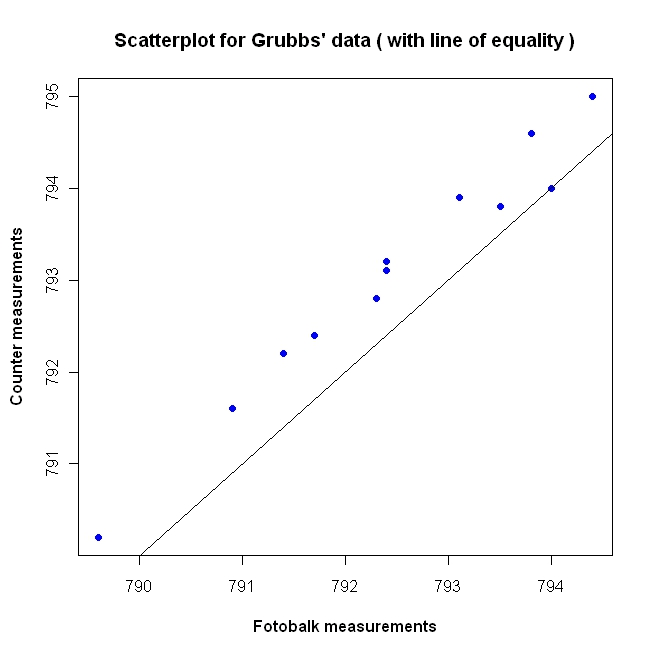
\includegraphics[width=130mm]{images/GrubbsScatter.jpeg}
			\caption{Scatter plot For Fotobalk and Counter Methods}\label{GrubbsScatter}
		\end{center}
	\end{figure}
	
	In light of shortcomings associated with scatterplots,
	\citet*{BA83} recommend a further analysis of the data. Firstly
	differences of measurements of two methods on the same subject
	should  be calculated, and then the average of those measurements
	(Table 2.1). These differences and averages are then plotted
	(Figure 2.2).
	
	
	
	
	The dashed line in Figure 2.2 alludes to the inter method bias
	between the two methods, as mentioned previously. Bland and Altman
	recommend the estimation of inter method bias by calculating the
	average of the differences. In the case of Grubbs data the inter
	method bias is $-0.6083$ metres per second.
	\newpage
	
	% latex table generated in R 2.6.0 by xtable 1.5-5 package
	% Thu Aug 27 16:31:52 2009
	\begin{table}[tbh]
		\begin{center}
			
			\begin{tabular}{rrrrr}
				\hline
				Round & Fotobalk [F] & Counter [C] & Differences [F-C] & Averages [(F+C)/2] \\
				\hline
				1 & 793.80 & 794.60 & -0.80 & 794.20 \\
				2 & 793.10 & 793.90 & -0.80 & 793.50 \\
				3 & 792.40 & 793.20 & -0.80 & 792.80 \\
				4 & 794.00 & 794.00 & 0.00 & 794.00 \\
				5 & 791.40 & 792.20 & -0.80 & 791.80 \\
				6 & 792.40 & 793.10 & -0.70 & 792.80 \\
				7 & 791.70 & 792.40 & -0.70 & 792.00 \\
				8 & 792.30 & 792.80 & -0.50 & 792.50 \\
				9 & 789.60 & 790.20 & -0.60 & 789.90 \\
				10 & 794.40 & 795.00 & -0.60 & 794.70 \\
				11 & 790.90 & 791.60 & -0.70 & 791.20 \\
				12 & 793.50 & 793.80 & -0.30 & 793.60 \\
				\hline
			\end{tabular}
			\caption{Fotobalk and Counter Methods: Differences and Averages}
		\end{center}
	\end{table}
	
	
	\begin{figure}[h!]
		\begin{center}
			\includegraphics[width=120mm]{images/GrubbsBAplot.jpeg}
			\caption{Bland Altman Plot For Fotobalk and Counter Methods}\label{GrubbsBA}
		\end{center}
	\end{figure}
	
	\newpage
	By inspection of the plot, it is also possible to compare the precision of each method. Noticeably the differences tend to
	increase as the averages increase.
	
	\subsection{Inspecting the Data}
	Bland-Altman plots are a powerful graphical methodology for making a visual assessment of the data. \citet*{BA83} express the motivation for this plot thusly:
	\begin{quote}
		"From this type of plot it is much easier to assess the magnitude
		of disagreement (both error and bias), spot outliers, and see
		whether there is any trend, for example an increase in
		(difference) for high values. This way of plotting the data is a
		very powerful way of displaying the results of a method comparison
		study."
	\end{quote}
	
	
	Figures 1.3 1.4 and 1.5 are three Bland-Altman plots derived from
	simulated data, each for the purpose of demonstrating how the plot
	would inform an analyst of trends that would adversely affect use
	of the recommended methodology. Figure 1.3 demonstrates how the
	Bland Altman plot would indicate increasing variance of
	differences over the measurement range. Figure 1.4 is an example
	of cases where the inter-method bias changes over the measurement
	range. This is known as proportional bias \citep{ludbrook97}.
	
	
	\begin{figure}[h!]
		\begin{center}
			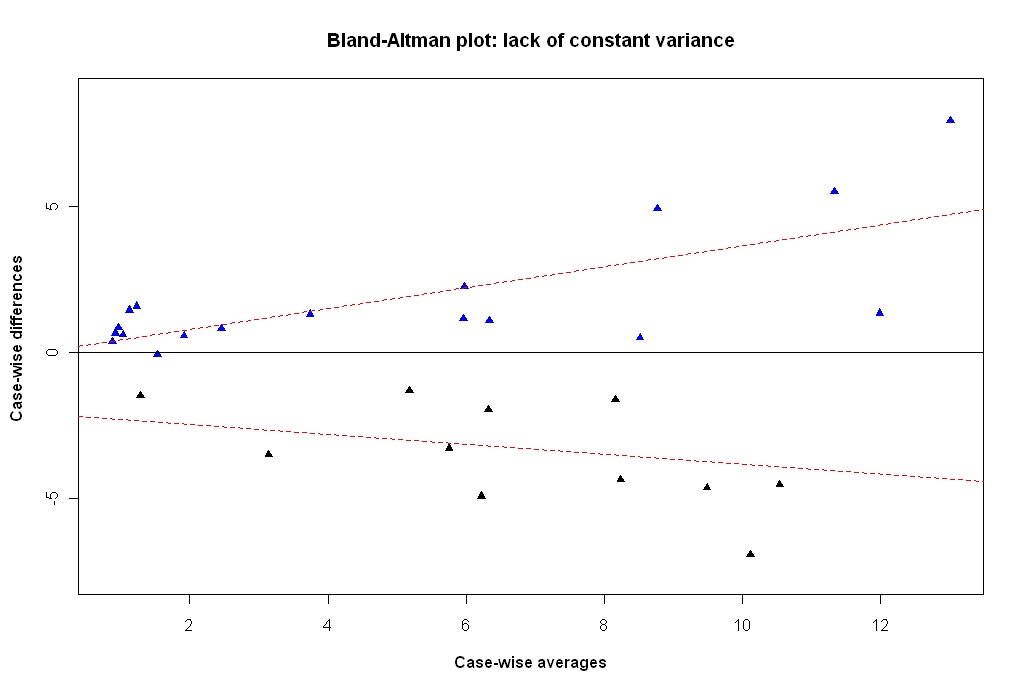
\includegraphics[width=125mm]{images/BAFanEffect.jpeg}
			\caption{Bland-Altman Plot demonstrating the increase of variance over the range}\label{BAFanEffect}
		\end{center}
	\end{figure}
	
	\begin{figure}[h!]
		\begin{center}
			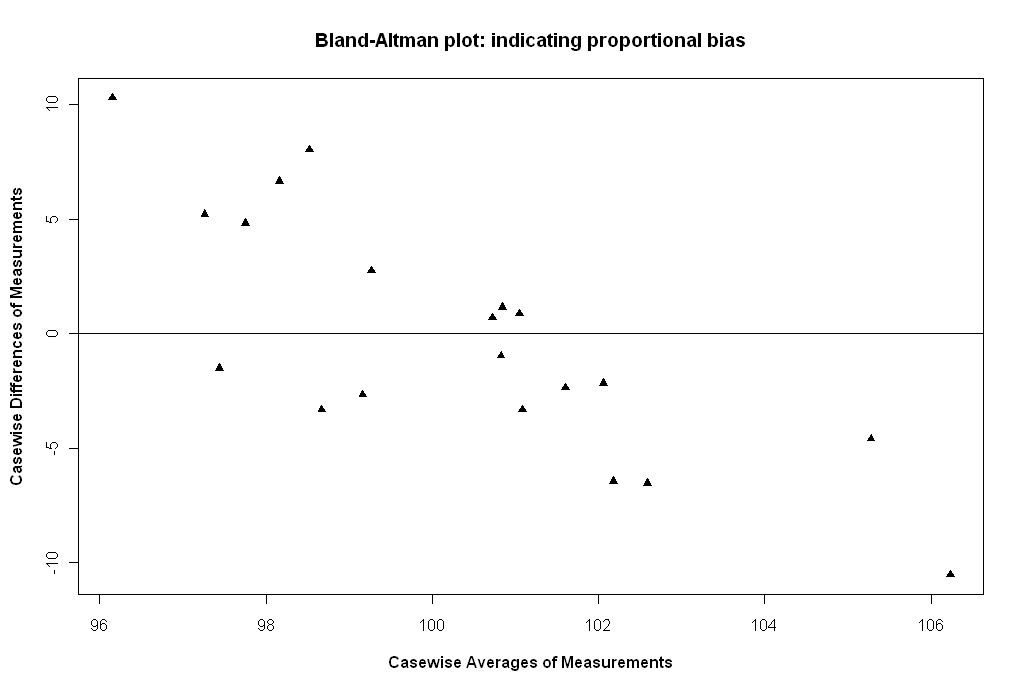
\includegraphics[width=125mm]{images/PropBias.jpeg}
			\caption{Bland-Altman Plot indicating the presence of proportional bias}\label{PropBias}
		\end{center}
	\end{figure}
	
	\newpage
	Figure 1.4 is an example of cases where the inter-method bias
	changes over the measurement range. This is known as\textit{ proportional
		bias} (Ludbrook, 1997). Both of these cases violate the assumptions
	necessary for further analysis using limits of agreement ,which
	shall be discussed later. The plot also can be used to identify
	outliers. An outlier is an observation that is numerically distant
	from the rest of the data. Classification thereof is a subjective
	decision in any analysis, but must be informed by the logic of the
	formulation. Figure 1.5 is a Bland Altman plot with two
	conspicuous observations, at the extreme left and right of the
	plot respectively.
	
	
	%\begin{figure}[h!]
	%	\begin{center}
	%		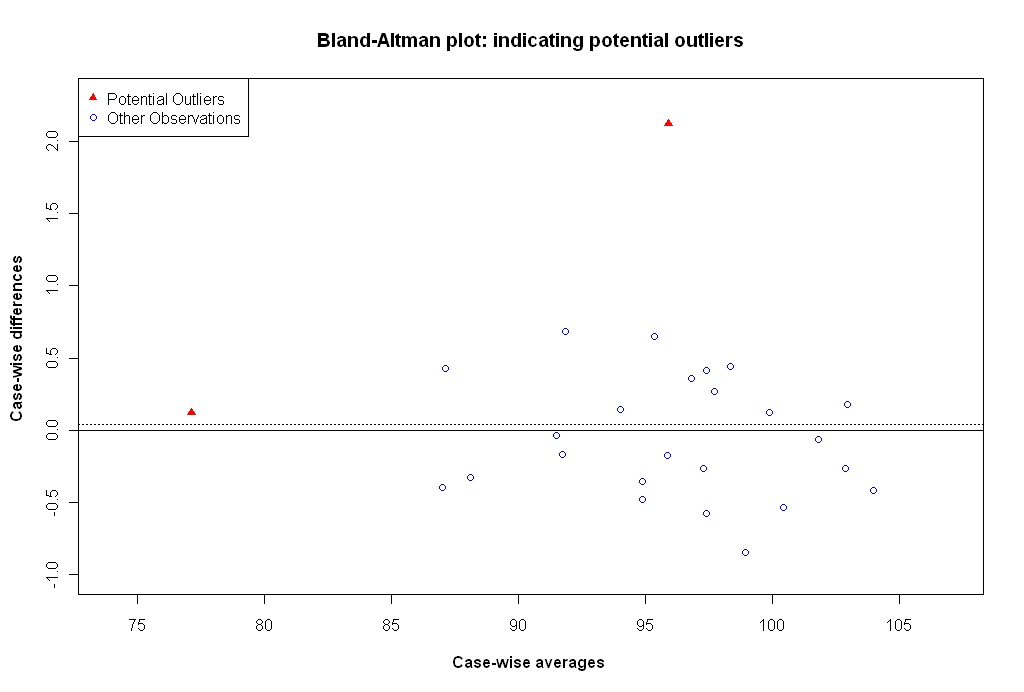
\includegraphics[width=125mm]{BAOutliers.jpeg}
	%		\caption{Bland-Altman Plot indicating the presence of Outliers}\label{PropBias}
	%	\end{center}
	%\end{figure}
	
	In the Bland-Altman plot, the horizontal displacement of any
	observation is supported by two independent measurements. Hence
	any observation , such as the one on the extreme right of figure
	1.5, should not be considered an outlier on the basis of a
	noticeable horizontal displacement from the main cluster. The one
	on the extreme left should be considered an outlier, as it has a
	noticeable vertical displacement from the rest of the
	observations.
	
	\citet*{BA99} do not recommend excluding outliers from analyses.
	However recalculation of the inter-method bias estimate , and
	further calculations based upon that estimate, are useful for
	assessing the influence of outliers.\citep{BA99} states that
	\emph{"We usually find that this method of analysis is not too
		sensitive to one or two large outlying differences."}
	
	\subsection{Limits of Agreement}
	\citet{BA86} introduces an elaboration of the plot, adding to the
	plot `limits of agreement' to the plot. These limits are based
	upon the standard deviation of the differences. The discussion
	shall be reverted to these limits of agreement in due course.
	
	\subsection{Variations of the Bland Altman Plot}
	\citet{BA99} remarks that it is possible to ignore the issue
	altogether, but the limits of agreement would wider apart than
	necessary when just lower magnitude measurements are considered.
	Conversely the limits would be too narrow should only higher
	magnitude measurements be used. To address the issue, they propose
	the logarithmic transformation of the data. The plot is then
	formulated as the difference of paired log values against their
	mean. \citet{BA99} acknowledge that this is not easy to interpret,
	and that it is not suitable in all cases.
	
	\citet{BA99} offers two variations of the Bland -Altman plot that
	are intended to overcome potential problems that the conventional
	plot would inappropriate for.
	
	The first variation is a plot of casewise differences as
	percentage of averages, and is appropriate when there is an
	increase in variability of the differences as the magnitude
	increases. The second variation is a plot of casewise ratios as
	percentage of averages.
	
	
	% When selecting this option the differences will be expressed as
	% percentage of the averages. This option is useful when there is an
	% increase in variability of the differences as the magnitude of the
	% measurement increases.
	
	
	
	
	% Plot ratios When this option is selected then the ratios of the
	% measurements will be plotted instead of the differences (avoiding
	% the need for log transformation). This option as well is useful
	% when there is an increase in variability of the differences as the
	% magnitude of the measurement increases.
	
	%----------------------------------------------------------------------------%
	\subsection{Agreement} Bland and Altman (1986) defined perfect
	agreement as the case where all of the pairs of rater data lie
	along the line of equality, where the line of equality is defined
	as the $45$ degree line passing through the origin(i.e. the $X=Y$
	line).
	
	Bland and Altman (1986)expressed this in the terms \emph{we want
		to know by how much the new method is likely to differ from the
		old; if this is not enough to cause problems in clinical
		interpretation we can replace the old method by the new or use the
		two interchangeably. How far apart measurements can be without
		causing difficulties will be a question of judgment. Ideally, it
		should be defined in advance to help in the interpretation of the
		method comparisonand to choose the sample size” .}
	%----------------------------------------------------------------------------%
	\subsection{Bias}
	Bland and Altman define bias a \emph{a consistent tendency for one
		method to exceed the other} and propose estimating its value
	by determining the mean of the differences. The variation about
	this mean shall be estimated by the  standard deviation of the
	differences. Bland and Altman remark that these estimates are based on the
	assumption that bias and variability are constant throughout the
	range of measures.
	%----------------------------------------------------------------------------%
	\subsection{Inappropriate assessment of Agreement}
	\subsubsection{Paired T tests} This method can be applied to test for
	statistically significant deviations in bias. This method can be
	potentially misused for method comparison studies.
	\\It is a poor measure of agreement when the rater's measurements
	are perpendicular to the line of equality[Hutson et al]. In this
	context, an average difference of zero between the two raters, yet
	the scatter plot displays strong negative correlation.
	\subsubsection{Inappropriate Methodologies} Use of the Pearson
	Correlation Coefficient , although seemingly intuitive, is not
	appropriate approach to assessing agreement of two methods.
	Arguments against its usage have been made repeatedly in the
	relevant literature. It is possible for two analytical methods to
	be highly correlated, yet have a poor level of agreement.
	\subsubsection{Pearson's Correlation Coefficient} It is well known that
	Pearson's correlation coefficient is a measure of the linear
	association between two variables, not the agreement between two
	variables (e.g., see Bland and Altman 1986)..This is a well known
	as a measure of linear association between two
	variables.Nonetheless this is not necessarily the same as
	Agreement. This method is considered wholly inadequate to assess
	agreement because it only evaluates only the association of two
	sets of observations.
	
	%----------------------------------------------------------------------------%
	\subsection{Inappropriate use of the Correlation Coefficient}
	It is intuitive when dealing with two sets of related data, i.e
	the results of the two raters,  to calculate the correlation
	coefficient (r). Bland and Altman attend to this in their $1999$
	paper.
	
	They present a data set from two sets of meters, and an
	accompanying scatterplot. An hypothesis test on the data set leads
	us to conclude that there is a relationship between both sets of
	meter measurements. The correlation coeffiecient is determined to
	be r =0.94.However, this high correlation does not mean that the
	two methods agree. It is possible to determine from the
	scatterplot that the intercept is not zero, a requirement for
	stating both methods have high agreement. Essentially, should two
	methods have highly correlated results, it does not follow that
	they have high agreement.
	
	%----------------------------------------------------------------------------%
	\subsection{Bland Altman Plot}
	Bland Altman have recommended the use of graphical techniques to
	assess agreement. Principally their method is calculating , for
	each pair of corresponding two methods of measurement of some
	underlying quantity, with no replicate measurements, the
	difference and mean. Differences are then plotted against the
	mean.
	
	\textbf{\textit{Hopkins}} argued that the bias in a subsequent Bland-Altman plot was
	due, in part, to using least-squares regression at the calibration
	phase.
	
	
	%This page also shows the standard deviation (SD) of the
	%differences between the two assay methods. The SD value is used to
	%calculate the limits of agreement, computed as the mean bias plus
	%or minus 1.96 times its SD.
	%----------------------------------------------------------------------------%
	\subsection{The Bland Altman Plot}
	In 1986 Bland and Altman published a paper in the Lancet proposing
	the difference plot for use for method comparison purposes. It has
	proved highly popular ever since. This is a simple, and widely
	used , plot of the differences of each data pair, and the
	corresponding average value. An important requirement is that the
	two measurement methods use the same scale of measurement.
	
	\subsubsection{scatter plots} The authors advise the
	use of scatter plots to identify outliers, and to determine if
	there is curvilinearity present. In the region of linearity
	,simple linear regression may yield results of interest.
	
	\subsection{Effect of Outliers} Another argument against
	the use of model I regression is based on outliers. Outliers can
	adversely influence the fitting of a regression model. Cornbleet
	and Cochrane compare a regression model influenced by an outlier
	with a model for the same data set, with the outlier excluded from
	the data set. A demonstration of the effect of outliers was made
	in Bland Altman's 1986 paper. However they discourage the
	exclusion of outliers.
	
	%----------------------------------------------------------------------------%
	\subsection{Limits Of Agreement}
	Bland and Altman proposed a pair of Limits of agreement. These
	limits are intended to demonstrate the range in which 95\% of the
	sample data should lie. The Limits of agreement centre on the
	average difference line and are 1.96 times the standard deviation
	above and below the average difference line.
	
	How this relates the overall population is unclear. It seems that
	it depends on an expert to decide whether or not the range of
	differences is acceptable. In a study A Bland-Altman plots compare
	two assay methods. It plots the difference between the two
	measurements on the Y axis, and the average of the two
	measurements on the X axis.
	
	The bias is computed as the average of the difference of paired
	assays.
	
	If one method is sometimes higher, and sometimes the other method
	is higher, the average of the differences will be close to zero.
	If it is not close to zero, this indicates that the two assay
	methods are producing different results systematically.
	
	\subsubsection{Precision of Limits of Agreement}
	The limits of agreement are estimates derived from the sample
	studied, and will differ from values relevant to the whole
	population. A different sample would give different limits of
	agreement. \citet*{BA86} advance a formulation for confidence
	intervals of the inter-method bias and the limits of agreement.
	These calculations employ quantiles of the `t' distribution with
	$n -1$ degrees of freedom.
	
	%This page also shows the standard deviation (SD) of the
	%differences between the two assay methods. The SD value is used to
	%calculate the limits of agreement, computed as the mean bias plus
	%or minus 1.96 times its SD.
	%----------------------------------------------------------------------------%
	\subsection{Appropriate Use of Limits of Agreement}
	Importantly \citet{BA99} makes the following point:
	\begin{quote}These estimates are meaningful only if we can assume
		bias and variability are uniform throughout the range of
		measurement, assumptions which can be checked graphically.
	\end{quote}
	
	The import of this statement is that , should the Bland Altman
	plot indicate that these assumptions are not met, then their
	entire methodology, as posited thus far, is inappropriate for use
	in a method comparison study. Again, in the context of potential
	outlier in the Grubbs data (figure 1.2), this raises the question
	on how to correctly continue.
	
	Carstensen attends to the issue of repeated data, using the
	expression replicate to express a repeated measurement on a
	subject by the same methods. Carstensen formulates the data as
	follows Repeated measurement - Arrangement of data into groups,
	based on the series of results of each subject.
	
	%----------------------------------------------------------------------------%
	\subsection{The Bland Altman Plot - Variations}
	Variations of the Bland Altman plot is the use of ratios, in the
	place of differences.
	\begin{equation}
	D_{i} = X_{i} - Y_{i}   \label{BA01}
	\end{equation}
	Altman and Bland suggest plotting the within subject differences $
	D = X_{1} - X_{2} $ on the ordinate versus the average of $x_{1}$
	and  $x_{2}$ on the abscissa.
	%----------------------------------------------------------------------------%
	\subsection{Pitman \& Morgan Test} This test assess tthe equaltiy
	of population vairances. Pitman's test tests for zero corrleation
	between the sums and products.
	
	Correlation between differences and means is a test statistics for
	the null hypothesis of equal variances given bivariate normality.
	%----------------------------------------------------------------------------%
	\subsection{Lin's Reproducibility Index} Lin proposes the use of a
	reproducibility index, called the Concordance Correlation
	Coefficent (CCC).While it is not strictly a measure of agreement
	as such, it can form part of an overall method comparision
	methodology.
	
	\section{Agreement}
	\begin{itemize}
		\item The FDA define precision as the \textit{closeness of agreement} (degree of
		scatter) between a series of measurements obtained from multiple
		sampling of the same homogeneous sample under prescribed
		conditions. 
		\item \textbf{Barnhart} describes precision as being further
		subdivided as either within-run, intra-batch precision or
		repeatability (which assesses precision during a single analytical
		run), or between-run, inter-batch precision or repeatability
		(which measures precision over time).
	\end{itemize}
	
	\section{Method Comparison Studies}
	
	Agreement between two methods of clinical measurement can be quantified using the differences between observations made using the two methods on the same subjects. The 95\% limits of agreement, estimated by mean difference +/- 1.96 standard deviation of the differences, provide an interval within which 95\% of differences between measurements by the two methods are expected to lie.
	
	\chapter{Introduction to MCS}
	\section{Outline of Thesis}
	Thus the study of method comparison is introduced. The intention of this thesis is to progress the
	study of method comparison studies, using a statistical method known as Linear mixed effects models.
	Chapter two shall describe linear mixed effects models, and how the use of the linear mixed
	effects models have so far extended to method comparison studies. Implementations of important existing work shall be presented, using the \texttt{R} programming language.
	
	In the first chapter the study of method comparison is introduced, while the second chapter provides a review of current methodologies. The intention of this thesis is to progress the study of method comparison studies, using a statistical method known as Linear mixed effects models.
	
	Chapter three shall describes linear mixed effects models, and how the use of the linear mixed effects models have so far extended to method comparison studies. Implementations of important existing work shall be presented, using the \texttt{R} programming language.
	
	Model diagnostics are an integral component of a complete statistical analysis.
	In chapter three model diagnostics shall be described in depth, with particular
	emphasis on linear mixed effects models, further to chapter two.
	
	For the fourth chapter, important linear mixed effects model diagnostic methods shall be extended to method comparison studies, and proposed methods shall be demonstrated on data sets that have become well known in literature on method comparison. The purpose is to both calibrate these methods and to demonstrate applications for them.
	The last chapter shall focus on robust measures of important parameters such as agreement.
	
	
	\section{Purposes of MCS}
	
	The  question being answered is not always clear, but is usually epxressed as an attempt to quantify the agreement
	between two methods (Bland and Altman 1995)
	
	Some lack of agreement between different methods of measurement is inevitable. What matters is the amount by which they
	disagree. we want to know by how much the new method is likely to differ from the old, so that it is not enough to cause
	problems in the mathematical interpretation we can preplace the old method by the new, or even use the two interchangably.
	
	
	It often happens that the same physical and chemical property can be measured in different ways. For example, one can determine
	For example, one can determine sodium in serum by flame atomic emission spectroscopy or by isotops dilution mass spectroscopy. The question arises as to whcih methd is better (Mandel 1991)
	
	In areas of inter-laboratory quality control, method comparisons, assay validations and individual bio-equivalence, etc, the agree between observations and target (reference) value is
	of interest (lin 2002)
	
	The purpose of comparing two methods of measurement of a continuous biological variable is to uncover systematic differences, not to point to
	similarities. (ludbrook 1997)
	
	In the pharmaceutical industry, measurement methods that measure the quantity of prdocuts are regulated. The FDA (U.S. Food and
	Drug Administration) requires that the manufacturer show equivalency prior to approving the new or alternatice method in quality control (Tan \& Inglewicz ,1999)
	
	\section{Discussion on Method Comparison Studies}
	
	The need to compare the results of two different measurement
	techniques is common in medical statistics.
	\\
	\\
	In particular, in medicine, new methods or devices that are
	cheaper, easier to use, or less invasive, are routinely developed.
	Agreement between a new method and a traditional reference or gold
	standard must be evaluated before the new one is put into
	practice. Various methodologies have been proposed for this
	purpose in recent years.
	
	Indications on how to deal with outliers in Bland Altman plots
	\\
	We wish to determine how outliers should be treated in a Bland
	Altman Plot
	\\
	In their 1983 paper they merely state that the plot can be used to
	'spot outliers'.
	\\
	In  their 1986 paper, Bland and Altman give an example of an
	outlier. They state that it could be omitted in practice, but make
	no further comments on the matter.
	\\
	In Bland and Altmans 1999 paper, we get the clearest indication of
	what Bland and Altman suggest on how to react to the presence of
	outliers. Their recommendation is to recalculate the limits
	without them, in order to test the difference with the calculation
	where outliers are retained.\\
	
	The span has reduced from 77 to 59 mmHg, a noticeable but not
	particularly large reduction.
	\\
	However, they do not recommend removing outliers. Furthermore,
	they say:
	\\
	We usually find that this method of analysis is not too sensitive
	to one or two large outlying differences.
	\\
	We ask if this would be so in all cases. Given that the limits of
	agreement may or may not be disregarded, depending on their
	perceived suitability, we examine whether it would possible that
	the deletion of an outlier may lead to a calculation of limits of
	agreement that are usable in all cases?
	\\
	Should an Outlying Observation be omitted from a data set? In
	general, this is not considered prudent.
	\\
	Also, it may be required that the outliers are worthy of
	particular attention themselves.
	\\
	Classifying outliers and recalculating We opted to examine this
	matter in more detail. The following points have to be considered
	\\how to suitably identify an outlier (in a generalized sense)
	\\Would a recalculation of the limits of agreement generally
	results in  a compacted range between the upper and lower limits
	of agreement?
	\subsection{Agreement} Bland and Altman (1986) define Perfect
	agreement as 'The case where all of the pairs of rater data lie
	along the line of equality'. The Line of Equality is defined as
	the 45 degree line passing through the origin, or X=Y on a XY
	plane.
	
	\subsection{Lack Of Agreement}
	\begin{enumerate}
		\item Constant Bias\item Proportional Bias
	\end{enumerate}
	
	\subsubsection*{Constant Bias} This is a form of systematic
	deviations estimated as the average difference between the test
	and the reference method
	
	
	\subsubsection*{Proportional Bias} Two methods may agree on
	average, but they may exhibit differences over a range of
	\section{Methods of assessing agreement}
	
	\begin{enumerate}
		\item Pearson's Correlation Coefficient\item Intraclass
		correlation coefficient \item Bland Altman Plot \item Bartko's
		Ellipse (1994) \item Blackwood Bradley Test \item Lin's
		Reproducibility Index \item Luiz Step function
	\end{enumerate}
	
	Bland and Altman attend to the issue of repeated measures in
	$1996$.
	\\
	Repeated measurements on several subjects can be used to quantify
	measurement error, the variation between measurements of the same
	quantity on the same individual.
	\\
	Bland and Altman discuss two metrics for measurement error; the
	within-subject standard deviation ,and the correlation
	coefficient.
	
	The above plot incorporates both the conventional limits of
	agreement ( the inner pair of dashed lines), the `t' limits of
	agreement ( the outer pair of dashed lines) centred around the
	inter-method bias (indicated by the full line). This plot is
	intended for expository purposes only, as the sample size is
	small.
	
	
	
	
	
	\subsection{Equivalence and Interchangeability}
	Limits of agreement are intended to analyse equivalence. How this
	is assessed is the considered judgement of the practitioner. In
	\citet{BA86} an example of good agreement is cited. For two
	methods of measuring `oxygen saturation', the limits of agreement
	are calculated as (-2.0,2.8).A practitioner would ostensibly find
	this to be sufficiently narrow.
	
	If the limits of agreement are not clinically important, which is
	to say that the differences tend not to be substantial, the two
	methods may be used interchangeably. \citet{DunnSEME} takes issue
	with the notion of `equivalence', remarking that while agreement
	indicated equivalence, equivalence does not reflect agreement.
	
	
	
	
	\section{Bland Altman Plots In Literature}
	\citet{mantha} contains a study the use of Bland Altman plots of
	44 articles in several named journals over a two year period. 42
	articles used Bland Altman's limits of agreement, wit the other
	two used correlation and regression analyses. \citet{mantha}
	remarks that 3 papers, from 42 mention predefined maximum width
	for limits of agreement which would not impair medical care.
	
	The conclusion of \citet{mantha} is that there are several
	inadequacies and inconsistencies in the reporting of results ,and
	that more standardization in the use of Bland Altman plots is
	required. The authors recommend the prior determination of limits
	of agreement before the study is carried out. This contention is
	endorsed by \citet{lin}, which makes a similar recommendation for
	the sample size, noting that\emph{sample sizes required either was
		not mentioned or no rationale for its choice was given}.
	
	\begin{quote}
		In order to avoid the appearance of "data dredging", both the
		sample size and the (limits of agreement) should be specified and
		justified before the actual conduct of the trial. \citep{lin}
	\end{quote}
	
	\citet{Dewitte} remarks that the limits of agreement should be
	compared to a clinically acceptable difference in measurements.
	%%%%%%%%%%%%%%%%%%%%%%%%%%%%%%%%%%%%%%%%%%%%%%%%%%%%%%%%%%%%%%%%%%%%%%%%%
	%4 Inappropriate assessment of Agreement       %%%%%%%%%%%%%%%%%%%%%%%%%%
	%%%%%%%%%%%%%%%%%%%%%%%%%%%%%%%%%%%%%%%%%%%%%%%%%%%%%%%%%%%%%%%%%%%%%%%%%
	
	
	\subsection{Gold Standard} This is considered to be the most
	accurate measurement of a particular parameter.
	
	measurements\section{Bland Altman Plot} Bland Altman have
	recommended the use of graphical techniques to assess agreement.
	Principally their method is calculating , for each pair of
	corresponding two methods of measurement of some underlying
	quantity, with no replicate measurements, the difference and mean.
	Differences are then plotted against the mean.
	
	
	Hopkins argued that the bias in a subsequent Bland-Altman plot was
	due, in part, to using least-squares regression at the calibration
	phase.
	
	\subsection{Bland Altman plots using 'Gold Standard' raters}
	According to Bland and Altman, one should use the methodology
	previous outlined, even when one of the raters is a Gold Standard.
	
	
	\subsection{Bias Detection}
	further to this method, the presence of constant bias may be
	indicated if the average value differences is not equal to zero.
	Bland and Altman does, however, indicate the indication of absence
	of bias does not provide sufficient information to allow a
	judgement as to whether or not one method can be substituted for
	another.
	
	
	
	
	\subsection{Limits Of Agreement}
	Bland and Altman proposed a pair of Limits of agreement. These
	limits are intended to demonstrate the range in which 95\% of the
	sample data should lie. The Limits of agreement centre on the
	average difference line and are 1.96 times the standard deviation
	above and below the average difference line.
	\\
	How this relates the overall population is unclear. It seems that
	it depends on an expert to decide whether or not the range of
	differences is acceptable. In a study A Bland-Altman plots compare
	two assay methods. It plots the difference between the two
	measurements on the Y axis, and the average of the two
	measurements on the X axis
	
	% introduces
	A third element of the Bland-Altman methodology, an interval known
	as `limits of agreement' is introduced in \citet*{BA86},
	(sometimes referred to in literature as 95\% limits of agreement).
	Limits of agreement are used to assess whether the two methods of
	measurement can be used interchangeably. \citet{BA86} refer to
	this as the `equivalence' of two measurement methods. It must be
	established clearly the specific purpose of the limits of
	agreement. \citet*{BA95} comment that the limits of agreement
	``how far apart measurements by the two methods were likely to be
	for most individuals'', a definition echoed in their 1999 paper:
	
	\begin{quote} ``We can then say that nearly all pairs
		of measurements by the two methods will be closer together than
		these extreme values, which we call 95\% limits of agreement.
		These values define the range within which most differences
		between measurements by the two methods will lie."
	\end{quote}
	
	The limits of agreement (LoA) are computed by the following
	formula:
	\begin{equation}
	LoA = \bar{d} \pm 1.96 S(d)
	\end{equation}
	with $\bar{d}$ as the estimate of the inter method bias, $S(d)$ as
	the standard deviation of the differences and 1.96 is the 95\%
	quantile for the standard normal distribution. (However, in some
	literature, 2 standard deviations are used instead for
	simplicity.) For the Grubbs `F vs C' comparison, these limits of
	agreement are calculated as -0.132 for the upper bound, and -1.08
	for the lower bound. Figure 1.9 shows the resultant Bland-Altman
	plot, with the limits of agreement shown in dashed lines.
	
	%
	%\begin{figure}[h!]
	%	\begin{center}
	%		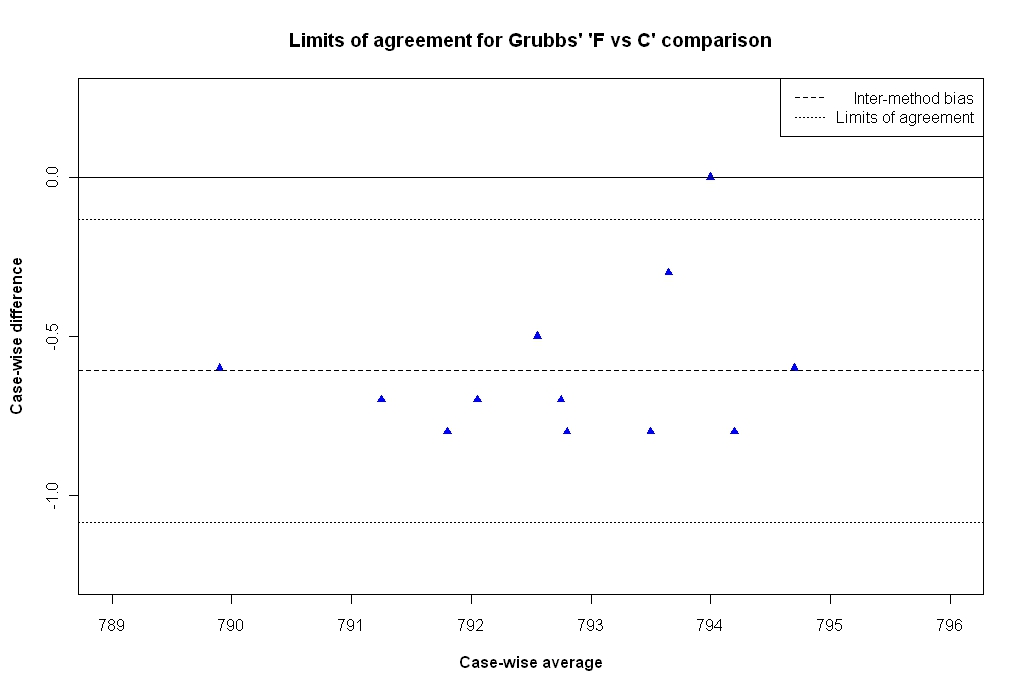
\includegraphics[width=125mm]{GrubbsBAplot-LOA.jpeg}
	%		\caption{Bland-Altman plot with limits of agreement}\label{GrubbsBAplot-noLOA}
	%	\end{center}
	%\end{figure}
	
	The limits of agreement methodology assumes a constant level of
	bias throughout the range of measurements. As \citet*{BA86} point
	out this may not be the case. Bland and Altman advises on how to
	calculate of confidence intervals for the inter-method bias and
	the limits of agreement. Importantly the authors recommend prior
	determination of what would and would constitute acceptable
	agreement, and that sample sizes should be predetermined to give
	an accurate conclusion.
	
	\begin{quote}
		`How far apart measurements can be without causing difficulties
		will be a question of judgment. Ideally, it should be defined in
		advance to help in the interpretation of the method comparison and
		to choose the sample size.'\citep{BA86}
	\end{quote}
	
	%\subsubsection{Small Sample Sizes} The limits of agreement are
	%estimates derived from the sample studied, and will differ from
	%values relevant to the whole population, hence the importance of a
	%suitably large sample size. A different sample would give
	%different limits of agreement. Student's t-distribution is a well
	%known probability distribution used in statistical inference for
	%normally distributed populations when the sample size is small
	%\citep{student,Fisher3}. Consequently, using 't' quantiles , as
	%opposed to standard normal quantiles, may give a more appropriate
	%calculation for limits of agreement when the sample size is small.
	%For sample size $n=12$ the `t' quantile is 2.2 and the limits of
	%agreement are (-0.074,-1.143).
	\citet{BA99} note the similarity of limits of agreement to
	confidence intervals, but are clear that they are not the same
	thing. Interestingly, they describe the limits as ``being like a
	reference interval."
	
	Limits of agreement have very similar construction to Shewhart
	control limits. The Shewhart chart is a well known graphical
	methodology used in statistical process control. Consequently
	there is potential for misinterpreting the limits of agreement as
	if equivalent to Shewhart control limits. Importantly the
	parameters used to determine the limits, the mean and standard
	deviation, are not based on any sample used for an analysis, but
	on the process's historical values, a key difference with
	Bland-Altman limits of agreement.
	
	\citet{BXC2008} regards the limits of agreement as a prediction
	interval for the difference between future measurements with the
	two methods on a new individual, but states that it does not fit
	the formal definition of a prediction interval, since the
	definition does not consider the errors in estimation of the
	parameters. Prediction intervals, which are often used in
	regression analysis, are estimates of an interval in which future
	observations will fall, with a certain probability, given what has
	already been observed. \citet{BXC2008} offers an alternative
	formulation, a $95\%$ prediction interval for the difference
	\begin{equation}
	\bar{d} \pm t_{(0.975, n-1)}S_{d} \sqrt{1+\frac{1}{n}}
	\end{equation}
	
	\noindent where $n$ is the number of subjects. Only for 61 or more
	subjects is there a quantile less than 2.
	
	\citet{luiz} describes limits of agreement as tolerance limits. A
	tolerance interval for a measured quantity is the interval in
	which a specified fraction of the population's values lie, with a
	specified level of confidence.
	
	%At least 100 historical
	%values must be used to determine the acceptable value (i.e the
	%process mean) and the process standard deviation. The principle
	%that the mean and variance of a large sample of a homogeneous
	%population is a close approximation of the population's mean and
	%variance justifies this.
	
	\subsection{Appropriate Use of Limits of Agreement}
	Importantly \citet{BA99} makes the following point:
	\begin{quote}These estimates are meaningful only if we can assume
		bias and variability are uniform throughout the range of
		measurement, assumptions which can be checked graphically.
	\end{quote}
	
	The import of this statement is that , should the Bland Altman
	plot indicate that these assumptions are not met, then their
	entire methodology, as posited thus far, is inappropriate for use
	in a method comparison study. Again, in the context of potential
	outlier in the Grubbs data (figure 1.2), this raises the question
	on how to correctly continue.
	\subsection{Problems with Limits of Agreement}
	
	Several problems have been highlighted regarding Limits of
	Agreement. One is the somewhat arbitrary manner in which they are
	constructed. While in essence a confidence interval, they are not
	constructed a such. They are designed for future values.
	\\
	The formulation is also heavily influenced by outliers. An Example
	in \citet*{BA83} demonstrates the effect of recalculating without
	a particular outlier. Refering to the VCF data set in the same
	paper, there is more than one outlier.
	
	
	\chapter{Linear Mixed effects Models}
	\section{Linear Mixed effects Models}
	A linear mixed effects (LME) model is a statistical model containing both fixed effects and random effects (random effects are also known as variance components). LME models are a generalization of the classical linear model, which contain fixed effects only. When the levels of factors are considered to be sampled from a population,
	and each level is not of particular interest, they are considered random quantities with associated variances.
	The effects of the levels, as described, are known as random effects. Random effects are represented by unobservable
	normally distributed random variables. Conversely fixed effects are considered non-random and the
	levels of each factor are of specific interest.
	%LME models are useful models when considering repeated measurements or grouped observations.
	
	\citet{Fisher4} introduced variance components models for use in genetical studies. Whereas an estimate for variance must take an non-negative value, an individual variance component, i.e.\ a component of the overall variance, may be negative.
	
	The methodology has developed since, including contributions from
	\citet{tippett}, who extend the use of variance components into linear models, and \citet{eisenhart}, who introduced the `mixed model' terminology and formally distinguished between mixed and random effects models. \citet{Henderson:1950} devised a methodology for deriving estimates for both the fixed effects and the random effects, using a set of equations that would become known as `mixed model equations' or `Henderson's equations'.
	LME methodology is further enhanced by Henderson's later works \citep{Henderson53, Henderson59,Henderson63,Henderson73,Henderson84a}. The key features of Henderson's work provide the basis for the estimation techniques.
	
	\citet{HartleyRao} demonstrated that unique estimates of the variance components could be obtained using maximum likelihood methods. However these estimates are known to be biased `downwards' (i.e.\ underestimated) , because of the assumption that the fixed estimates are known, rather than being estimated from the data. \citet{PattersonThompson} produced an alternative set of estimates, known as the restricted maximum likelihood (REML) estimates, that do not require the fixed effects to be known. Thusly there is a distinction the REML estimates and the original estimates, now commonly referred to as ML estimates.
	
	\citet{LW82} provides a form of notation for notation for LME models that has since become the standard form, or the basis for more complex formulations. Due to computation complexity, linear mixed effects models have not seen widespread use until many well known statistical software applications began facilitating them. SAS Institute added PROC MIXED to its software suite in 1992 \citep{singer}. \citet{PB} described how to compute LME models in the \texttt{S-plus} environment.
	
	Using Laird-Ware form, the LME model is commonly described in matrix form,
	\begin{equation}
	y = X\beta + Zb + \epsilon
	\label{LW}
	\end{equation}
	
	\noindent where $y$ is a vector of $N$ observable random variables, $\beta$ is a vector of $p$ fixed effects, $X$ and $Z$ are $N \times p$ and $N \times q$ known matrices, and $b$ and $\epsilon$  are vectors of $q$ and $N,$ respectively, random effects such that $\mathrm{E}(b)=0, \ \mathrm{E}(\epsilon)=0$
	and
	%	\[
	%	\mathrm{var}
	%	\begin{pmatrix}{
	%		b \cr
	%		\epsilon }  =
	%	\begin{pmatrix}{
	%		D & 0 \cr
	%		0 & \Sigma }
	%	\]
	where $D$ and $\Sigma$ are positive definite matrices parameterized by an unknown variance component parameter vector $ \theta.$ The variance-covariance matrix for the vector of observations $y$ is given by $V = ZDZ^{\prime}+ \Sigma.$ This implies $y \sim(X\beta, V) = (X\beta,ZDZ^{\prime}+ \Sigma)$. It is worth noting that $V$ is an $n \times n$ matrix, as the dimensionality becomes relevant later on. The notation provided here is generic, and will be adapted to accord with complex formulations that will be encountered in due course.
	
	%\subsection{Likelihood and estimation}
	
	% Likelihood is the hypothetical probability that an event that has already occurred would yield a specific outcome. Likelihood differs from probability in that probability refers to future occurrences, while likelihood refers to past known outcomes.
	
	% The likelihood function ($L(\theta)$)is a fundamental concept in statistical inference. It indicates how likely a particular population is to produce an observed sample. The set of values that maximize the likelihood function are considered to be optimal, and are used as the estimates of the parameters. For computational ease, it is common to use the logarithm of the likelihood function, known simply as the log-likelihood ($\ell(\theta)$).
	
	
	\subsection{Estimation}
	Estimation of LME models involve two complementary estimation issues'; estimating the vectors of the fixed and random effects estimates $\hat{\beta}$ and $\hat{b}$ and estimating the variance covariance matrices $D$ and $\Sigma$.
	Inference about fixed effects have become known as `estimates', while inferences about random effects have become known as `predictions'. The most common approach to obtain estimators are Best Linear Unbiased Estimator (BLUE) and Best Linear Unbiased Predictor (BLUP). For an LME model given by (\ref{LW}), the BLUE of $\hat{\beta}$ is given by
	\[\hat{\beta} = (X^\prime V^{-1}X)^{-1}X^\prime V^{-1}y,\]whereas the BLUP of $\hat{b}$ is given by
	\[\hat{b} = DZ^{\prime} V^{-1} (y-X\hat{\beta}).\]
	
	
	
	\subsubsection{Estimation of the fixed parameters}
	
	The vector $y$ has marginal density $y \sim \mathrm{N}(X \beta,V),$ where $V = \Sigma + ZDZ^\prime$ is specified through the variance component parameters $\theta.$ The log-likelihood of the fixed parameters $(\beta, \theta)$ is
	\begin{equation}
	\ell (\beta, \theta|y) =
	-\frac{1}{2} \log |V| -\frac{1}{2}(y -
	X \beta)'V^{-1}(y -
	X \beta), \label{Likelihood:MarginalModel}
	\end{equation}
	and for fixed $\theta$ the estimate $\hat{\beta}$ of $\beta$ is obtained as the solution of
	\begin{equation}
	(X^\prime V^{-1}X) {\beta} = X^\prime V^{-1}y.
	\label{mle:beta:hat}
	\end{equation}
	
	Substituting $\hat{\beta}$ from (\ref{mle:beta:hat}) into $\ell(\beta, \theta|y)$ from (\ref{Likelihood:MarginalModel}) returns the \emph{profile} log-likelihood
	\begin{eqnarray*}
		\ell_P(\theta \mid y) &=& \ell(\hat{\beta}, \theta \mid y) \\
		&=& -\frac{1}{2} \log |V| -\frac{1}{2}(y - X \hat{\beta})'V^{-1}(y - X \hat{\beta})
	\end{eqnarray*}
	of the variance parameter $\theta.$ Estimates of the parameters $\theta$ specifying $V$ can be found by maximizing $\ell_P(\theta \mid y)$ over $\theta.$ These are the ML estimates.
	
	For REML estimation the \emph{restricted} log-likelihood is defined as
	\[
	\ell_R(\theta \mid y) =
	\ell_P(\theta \mid y) -\frac{1}{2} \log |X^\prime VX |.
	\]
	%\subsubsection{Likelihood estimation techniques}
	%Maximum likelihood and restricted maximum likelihood have become the most common strategies
	%for estimating the variance component parameter $\theta.$ Maximum likelihood estimation obtains
	%parameter estimates by optimizing the likelihood function.
	%To obtain ML estimate the likelihood is constructed as a function of the parameters in the specified LME model.
	% The maximum likelihood estimates (MLEs) of the parameters are the values of the arguments that maximize the likelihood function.
	
	The REML approach does not base estimates on a maximum likelihood fit of all the information, but instead uses a likelihood function derived from a data set, transformed to remove the irrelevant influences \citep{REMLDefine}.
	Restricted maximum likelihood is often preferred to maximum likelihood because REML estimation reduces the bias in the variance component by taking into account the loss of degrees of freedom that results
	from estimating the fixed effects in $\boldsymbol{\beta}$. Restricted maximum likelihood also handles high correlations more effectively, and is less sensitive to outliers than maximum likelihood.  The problem with REML for model building is that the likelihoods obtained for different fixed effects are not comparable. Hence it is not valid to compare models with different fixed effects using a likelihood ratio test or AIC when REML is used to
	estimate the model. Therefore models derived using ML must be used instead.
	
	\subsubsection{Estimation of the random effects}
	
	The established approach for estimating the random effects is to use the best linear predictor of $b$ from $y,$ which for a given $\beta$ equals $DZ^\prime V^{-1}(y - X \beta).$ In practice $\beta$ is replaced by an estimator such as $\hat{\beta}$ from (\ref{mle:beta:hat}) so that $\hat{b} = DZ^\prime V^{-1}(y - X \hat{\beta}).$ Pre-multiplying by the appropriate matrices it is straightforward to show that these estimates $\hat{\beta}$ and $\hat{b}$ satisfy the equations in (\ref{Henderson:Equations}).
	
	\subsubsection{Algorithms for likelihood function optimization}Iterative numerical techniques are used to optimize the log-likelihood function and estimate the covariance parameters $\theta$. The procedure is subject to the constraint that $R$ and $D$ are both positive definite. The most common iterative algorithms for optimizing the likelihood function are the Newton-Raphson method, which is the preferred method, the expectation maximization (EM) algorithm and the Fisher scoring methods.
	
	The EM algorithm, introduced by \citet{EM}, is an iterative technique for maximizing complicated likelihood functions. The algorithm alternates between performing an expectation (E) step
	and the maximization (M) step. The `E' step computes the expectation of the log-likelihood evaluated using the current
	estimate for the variables. In the `M' step, parameters that maximize the expected log-likelihood, found on the previous `E' step, are computed. These parameter estimates are then used to determine the distribution of the variables in the next `E' step. The algorithm alternatives between these two steps until convergence is reached.
	
	The main drawback of the EM algorithm is its slow rate of
	convergence. Consequently the EM algorithm is rarely used entirely in LME estimation,
	instead providing an initial set of values that can be passed to
	other optimization techniques.
	
	The Newton Raphson (NR) method is the most common, and recommended technique for ML and
	REML estimation. The NR algorithm minimizes an objective function defines as $-2$ times the log likelihood for the covariance parameters $\theta$. At every iteration the NR algorithm requires the
	calculation of a vector of partial derivatives, known as the gradient, and the second derivative matrix with respect to the covariance parameters. This is known as the observed Hessian matrix. Due to the Hessian matrix, the NR algorithm is more time-consuming, but convergence is reached with fewer iterations compared to the EM algorithm. The Fisher scoring algorithm is an variant of the NR algorithm that is more numerically stable and likely to converge, but not recommended to obtain final estimates.
	
	
	%------------------------------------------------------------------------------%
	\subsection{Formulation of the response vector}
	Information of individual $i$ is recorded in a response vector $\boldsymbol{y}_{i}$. The response vector is constructed by stacking the response of the $2$ responses at the first instance, then the $2$ responses at the second instance, and so on. Therefore the response vector is a $2n_{i} \times 1$ column vector.
	The covariance matrix of $\boldsymbol{y_{i}}$ is a $2n_{i} \times 2n_{i}$ positive definite matrix $\boldsymbol{\Omega}_{i}$.
	
	Consider the case where three measurements are taken by both methods $A$ and $B$, $\boldsymbol{y}_{i}$ is a $6 \times 1$ random vector describing the $i$th subject.
	\[
	\boldsymbol{y}_{i} = (y_{i}^{A1},y_{i}^{B1},y_{i}^{A2},y_{i}^{B2},y_{i}^{A3},y_{i}^{B3}) \prime
	\]
	
	The response vector $\boldsymbol{y_{i}}$ can be formulated as an LME model according to Laird-Ware form.
	\begin{eqnarray*}
		\boldsymbol{y_{i}} = \boldsymbol{X_{i}\beta}  + \boldsymbol{Z_{i}b_{i}} + \boldsymbol{\epsilon_{i}}\\
		\boldsymbol{b_{i}} \sim \mathcal{N}(\boldsymbol{0,D})\\
		\boldsymbol{\epsilon_{i}} \sim \mathcal{N}(\boldsymbol{0,R_{i}})
	\end{eqnarray*}
	
	Information on the fixed effects are contained in a three dimensional vector $\boldsymbol{\beta} = (\beta_{0},\beta_{1},\beta_{2})\prime$. For computational purposes $\beta_{2}$ is conventionally set to zero. Consequently $\boldsymbol{\beta}$ is the solutions of the means of the two methods, i.e. $E(\boldsymbol{y}_{i})  = \boldsymbol{X}_{i}\boldsymbol{\beta}$. The variance covariance matrix $\boldsymbol{D}$ is a general $2 \times 2$ matrix, while $\boldsymbol{R}_{i}$ is a $2n_{i} \times 2n_{i}$ matrix.
	
	%------------------------------------------------------------------------------%
	\subsection{Decomposition of the response covariance matrix}
	
	The variance covariance structure can be re-expressed in the following form,
	\[
	\mbox{Cov}(\mbox{y}_{i}) = \boldsymbol{\Omega_{i}} = \boldsymbol{Z}_{i}\boldsymbol{D}\boldsymbol{Z}_{i}^\prime + \boldsymbol{R_{i}}.
	\]
	
	$\boldsymbol{R_{i}}$ can be shown to be the Kronecker product of a correlation matrix $\boldsymbol{V}$ and $\boldsymbol{\Lambda}$. The correlation matrix $\boldsymbol{V}$ of the repeated measures on a given response variable is assumed to be the same for all response variables. Both \citet{hamlett} and \citet{lam} use the identity matrix, with dimensions $n_{i} \times n_{i}$ as the formulation for $\boldsymbol{V}$. \citet{ARoy2009} remarks that, with repeated measures, the response for each subject is correlated for each variable, and that such correlation must be taken into account in order to produce a valid inference on correlation estimates.  \citet{ARoy20092006} proposes various correlation structures may be assumed for repeated measure correlations, such as the compound symmetry and autoregressive structures, as alternative to the identity matrix.
	
	However, for the purposes of method comparison studies, the necessary estimates are currently only determinable when the identity matrix is specified, and the results in \citet{ARoy2009} indicate its use.
	
	For the response vector described, \citet{hamlett} presents a detailed covariance matrix. A brief summary shall be presented here only. The overall variance matrix is a $6 \times 6$ matrix composed of two types of $2 \times 2$ blocks. Each block represents one separate time of measurement.
	
	\[
	\boldsymbol{\Omega}_{i} = \left(
	\begin{array}{ccc}
	\boldsymbol{\Sigma} & \boldsymbol{D} & \boldsymbol{D}\\
	\boldsymbol{D} & \boldsymbol{\Sigma} & \boldsymbol{D}\\
	\boldsymbol{D} & \boldsymbol{D} & \boldsymbol{\Sigma}\\
	\end{array}\right)
	\]
	
	The diagonal blocks are $\Sigma$, as described previously. The $2 \times 2$ block diagonal matrix in $\boldsymbol{\Omega}$ gives $\boldsymbol{\Sigma}$. $\boldsymbol{\Sigma}$ is the sum of the between-subject variability $\boldsymbol{D}$ and the within subject variability $\boldsymbol{\Lambda}$.
	
	$\boldsymbol{\Omega_{i}}$ can be expressed as
	\[
	\boldsymbol{\Omega_{i}} = \boldsymbol{Z}_{i}\boldsymbol{D}\boldsymbol{Z}_{i}^\prime + ({\boldsymbol{I_{n_{i}}} \otimes \boldsymbol{\Lambda}}).
	\]
	The notation $\mbox{dim}_{n_{i}}$ means an $n_{i} \times n_{i}$ diagonal block.
	
	\subsection{Correlation terms}
	\citet{hamlett} demonstrated how the between-subject and within subject variabilities can be expressed in terms of
	correlation terms.
	
	\[
	\boldsymbol{D} = \left( \begin{array}{cc}
	\sigma^2_{A}\rho_{A} & \sigma_{A}\sigma_{b}\rho_{AB}\delta \\
	\sigma_{A}\sigma_{b}\rho_{AB}\delta & \sigma^2_{B}\rho_{B}\\
	
	\end{array}\right)
	\]
	
	\[
	\boldsymbol{\Lambda} = \left(
	\begin{array}{cc}
	\sigma^2_{A}(1-\rho_{A}) & \sigma_{AB}(1-\delta)  \\
	\sigma_{AB}(1-\delta) & \sigma^2_{B}(1-\rho_{B}) \\
	\end{array}\right).
	\]
	
	$\rho_{A}$ describe the correlations of measurements made by the method $A$ at different times. Similarly $\rho_{B}$ describe the correlation of measurements made by the method $B$ at different times. Correlations among repeated measures within the same method are known as intra-class correlation coefficients. $\rho_{AB}$ describes the correlation of measurements taken at the same same time by both methods. The coefficient $\delta$ is added for when the measurements are taken at different times, and is a constant of less than $1$ for linked replicates. This is based on the assumption that linked replicates measurements taken at the same time would have greater correlation than those taken at different times. For unlinked replicates $\delta$ is simply $1$. \citet{hamlett} provides a useful graphical depiction of the role of each correlation coefficients.
	
	
	
	
	
	
	
	
	
	\bibliography{DB-txfrbib}
	\chapter{LME Likelihood}
	\section{One Way ANOVA}
	\subsection{Page 448}
	Computing the variance of $\hat{\beta}$
	\begin{eqnarray}
	\mbox{var}(\hat{\beta}) = (X^{\prime}V^{-1}X)^-1
	\end{eqnarray}
	It is not necessary to compute $V^{-1}$ explicitly.
	
	\begin{eqnarray}
	V^{-1}X &= \Sigma^{1}{X-Z()Z^{\prime}\Sigma^{-1}X} \\
	&= \Sigma^{-1}(X-Zb_{x})
	\end{eqnarray}
	
	The estimate $b_{x}$ is the same term obtained from the random effects model; $X = Zb_{x} + e$, using $X$ as an outcome variable.
	This formula is convenient in applications where $b_{x}$ can be easily computed. Since $X$ is a matrix of $p$ columns, $b_{x}$ can simple be computed column by column. according to the columns of $X$.
	\subsection{Page 448- simple example}
	Consider a simple model of the form;
	\begin{equation*}
	y_{ij} = \mu + \beta_{i} + \epsilon_{ij}.
	\end{equation*}
	
	The iterative procedure is as follows Evaluate the individual group mean $\bar{y_{i}}$ and variance $\hat{Sigma^2}_{i}$. Then use the variance of the group means as an estimate of the $\sigma^2_{b}$. The average of the the variances of the groups is the initial estimate of the $\sigma^2_{e}$.
	\subsubsection{Iterative procedure}
	
	The iterative procedure comprises two steps, with $0$ as the first approximation of $b_{i}$.
	
	The first step is to compute $\lambda$, the ratio of variabilities,
	
	\begin{equation*}
	\lambda = \frac{\sigma^2_{b}}{\sigma^2_{e}}
	\end{equation*}
	
	\begin{eqnarray*}
		\mu = \frac{1}{N} \sum_{ij} (y_{ij} - b_{i}) \\
		b_{i} = \frac{n(\bar{y_{i}}-\mu)}{n+ \lambda} \\
	\end{eqnarray*}
	
	
	The second step is to updat $sigma^2_{e}$
	
	\begin{equation}
	\sigma^2_{e} = \frac{e^{\prime}e}{N-df}
	\end{equation}
	
	where $e$ is the vector of $e_{ij} = y_{ij}-\mu-b_{i}$ and $df =
	qn / n+\lambda$ and
	\begin{equation}
	\sigma^{2}_{b} = \frac{1}{q} \sum_{i=1}^{q} b_{1}^2 +
	(\frac{n}{\sigma^2_{e}}+\frac{1}{\sigma^2_{b}})^{-1}
	\end{equation}
	
	\subsubsection{Worked Example}
	
	Further to [pawitan 17.1] the initial estimates for variability
	are $\sigma^{2}_{b} = 1.7698$ and $\sigma^{2}_{e} = 0.3254$. At
	convergence the following results are obtained.
	\\
	n=16, q=5
	\begin{eqnarray*}
		\hat{\mu} = \bar{y} = 14.175 \\
		\hat{\sigma}^2 = 0.325\\
		\hat{\sigma}^2_{b} = 1.395\\
		\sigma  = 0.986 \\
	\end{eqnarray*}
	At convergene the following estimates are obtained,
	\begin{eqnarray*}
		\hat{\mu} = 14.1751 \\
		\hat{b}= (-0.6211, 0.2683,1.4389,-1.914,0.8279)\\
		\hat{\sigma}^2_{b} = 1.3955\\
		\hat{\sigma}^2_{e} = 0.3254\\
	\end{eqnarray*}
	
	
	\subsection{Extention to several random effects}
	[pawitan section 17.7]
	
	
	
	
	
	
	\section{Classical model for single measurements}
	The classical model is based on measurements $y_{mi}$
	by method $m=1,2$ on item $i = 1,2 \ldots$
	
	\[y_{mi} + \alpha_{m} + \mu_{i} + e_{mi}\]
	
	\[e_{mi} \sim \mathcal{n} (0,\sigma^2_m)\]
	
	Even though the separate variances can not be
	identified, their sum can be estimated by the empirical variance of the differences.
	
	Like wise the separate $\alpha$ can not be
	estimated, only theiir difference can be estimated as
	$\bar{D}$
	
	
	In the first instance, we require a simple model to describe a measurement by method $m$. We use the term $item$ to denote an individual, subject or sample, to be measured, being randomly sampled from a population. Let $y_{mi}$ be the measurement for item $i$ made by method $m$.
	
	\[ y_{mi} = \alpha_{m} + \mu_{i} + e_{mi}  \]
	
	\begin{itemize}
		\item $\alpha_m$ is the fixed effect associated with method $m$,
		\item $\mu_i$ is the true value for subject $i$ (fixed effect),
		\item $e_{mi}$ is a
		random effect term for errors with $e_{mi}  \sim \mathcal{N}(0,\sigma^2_m)$. \end{itemize}.
	
	This model implies that the difference between the paired measurements can be expressed as
	
	\[ d_{i} = y_{1i} - y_{2i} \sim \mathcal{N} (\alpha_{1} - \alpha_{2}, \sigma^2_{1} - \sigma^2_{2}). \]
	
	Importantly, this is independent of the item levels $\mu_i$. As the case-wise differences are of interest, the parameters of interest are the fixed effects for methods $\alpha_{m}$.
	
	\[ y_{mi} =  \alpha_{m}  + \mu_{i} + e_{mi}  \]
	
	
	
	
	
	Importantly these variance covariance structures are central to ARoy2009 methodology.
	
	
	\citet{ARoy2009} proposes a series of hypothesis tests based on these matrices as part of her methodology. These tests shall be reverted to in due course.
	
	The standard deviation of the differences of variables $a$ and $b$ is computed as
	\[
	\mbox{var}(a - b) = \mbox{var} ( a )  + \mbox{var} ( b ) - 2\mbox{cov} ( a ,b )
	\]
	
	Hence the variance of the difference of two methods, that allows for the calculation of the limits of agreement, can be calculated as
	
	\[
	\mbox{var}(d) = \omega^2_1  + \omega^2_2 - 2 \times \omega_12
	\]
	
	
	
	
	
	\section{Sampling}
	\emph{
		One important feature of replicate observations is that they should be independent
		of each other. In essence, this is achieved by ensuring that the observer makes each
		measurement independent of knowledge of the previous value(s). This may be difficult
		to achieve in practice.} (Check who said this
	)
	
	
	
	
	
	
	
	\section{Conclusion}
	\citet{BXC2008} and \citet{AARoy20092009} highlight the need for method comparison methodologies suitable for use in the presence of replicate measurements. \citet{AARoy20092009} presents a comprehensive methodology for assessing the agreement of two methods, for replicate measurements. This methodology has the added benefit of overcoming the problems of unbalanced data and unequal numbers of replicates. Implementation of the methodology, and interpretation of the results, is relatively easy for practitioners who have only basic statistical training. Furthermore, it can be shown that widely used existing methodologies, such as the limits of agreement, can be incorporated into ARoy2009's methodology.
	%=========================================================================================================================================== %
	%=========================================================================================================================================== %
	
	\section*{Permutation Test, Power Tests and Missing Data }
	
	This section explores topics such as dependent variable simulation and power analysis, introduced by Galecki \& Burzykowski (2013), and implementable with their \textbf{\textit{nlmeU}} \texttt{R} package.
	Using the \textbf{\textit{predictmeans}} \texttt{R} package, it is possible to perform permutation t-tests for coefficients of (fixed) effects and permutation F-tests.
	
	The matter of missing data has not been commonly encountered in either Method Comparison Studies or Linear Mixed Effects Modelling. However ARoy2009 (2009) deals with the relevant assumptions regrading missing data. Galecki \& Burzykowski (2013) approaches the subject of missing data in LME Modelling. The \textbf{\textit{nlmeU}} package includes the \texttt{patMiss} function, which ``\textit{allows to compactly present pattern of missing data in a given vector/matrix/data
		frame or combination of thereof}".
	
	
	%================================================%
	
	\chapter{General Appendices}
	$\Lambda = \frac{\mbox{max}_{H_{0}}L}{\mbox{max}_{H_{1}}L}$
	
	
	
	%----------------------------------------------------------------------------------------------%
	
	%http://blog.minitab.com/blog/adventures-in-statistics/why-you-need-to-check-your-residual-plots-for-regression-analysis
	In the graph above, you can predict non-zero values for the residuals based on the fitted value. For example, a fitted value of 8 has an expected residual that is negative. Conversely, a fitted value of 5 or 11 has an expected residual that is positive.
	
	The non-random pattern in the residuals indicates that the deterministic portion (predictor variables) of the model is not capturing some explanatory information that is “leaking” into the residuals. The graph could represent several ways in which the model is not explaining all that is possible. 
	
	Possibilities include:
	
	\begin{itemize}
		\item A missing variable
		\item A missing higher-order term of a variable in the model to explain the curvature
		\item A missing interction between terms already in the model
	\end{itemize}
	
	
	Identifying and fixing the problem so that the predictors now explain the information that they missed before should produce a good-looking set of residuals!
	
	In addition to the above, here are two more specific ways that predictive information can sneak into the residuals:
	
	The residuals should not be correlated with another variable. If you can predict the residuals with another variable, that variable should be included in the model. In Minitab’s regression, you can plot the residuals by other variables to look for this problem.
	
	\noindent \textbf{Autocorrelation} \\
	Adjacent residuals should not be correlated with each other (\textbf{autocorrelation}). If you can use one residual to predict the next residual, there is some predictive information present that is not captured by the predictors. Typically, this situation involves time-ordered observations. For example, if a residual is more likely to be followed by another residual that has the same sign, adjacent residuals are positively correlated. You can include a variable that captures the relevant time-related information, or use a time series analysis. 
	
	In Minitab’s regression, you can perform the \textbf{\textit{Durbin-Watson} }test to test for autocorrelation.
	
	\section{Repeated Measurements}
	
	In cases where there are repeated measurements by each of the two
	methods on the same subjects , Bland Altman suggest calculating
	the mean for each method on each subject and use these pairs of
	means to compare the two methods.
	The estimate of bias will be unaffected using this approach, but
	the estimate of the standard deviation of the differences will be
	too small, because of the reduction of the effect of repeated
	measurement error. Bland Altman propose a correction for this.
	Carstensen attends to this issue also, adding that another
	approach would be to treat each repeated measurement separately.
	
	
	%%%%%%%%%%%%%%%%%%%%%%%%%%%%%%%%%%%%%%%%%%%%%%%%%%%%%%%%%%%%%%%%%%%%%%%%%%%%%%%%%%%%%%%%%%%%%%%%%%%%%%%%%%%%%%%
	
	In this model , the variances of the random effects must depend on
	$m$, since the different methods do not necessarily measure on the
	same scale, and different methods naturally must be assumed to
	have different variances. \citet{BXC2004} attends to the issue of
	comparative variances.
	%----------------------------------------------------------------------------%
	\section{Lin's Reproducibility Index} Lin proposes the use of a
	reproducibility index, called the Concordance Correlation
	Coefficent (CCC).While it is not strictly a measure of agreement
	as such, it can form part of an overall method comparision
	methodology.
	
	\section{Overview}
	\begin{enumerate}
		\item Extending deletion diagnostics to LMEs
		\item Christensen et al
		\item Haslett hayes
		\item Schabenberger
		\item Tewomir
	\end{enumerate}
	
	\begin{enumerate}
		\item Residual Diagnostics
		\begin{enumerate}
			\item Marginal and Conditional Diagnostics
			\item Scaled Residuals
		\end{enumerate}
		
		\item Influence Diagnostics
		\begin{enumerate}
			\item Underlying Concepts
			\item Managing the Covariance Parameters
			\item Predicted Values, PRESS Residual and the PRESS Statistic
			\item Leverage
			\item Internally and Externally Studentized Residuals
			\item DFFITs and MDFFITs
			\item Covariance Ratio and Trace
			\item Likelihood Distance
			\item Non-iterative Update Procedures
		\end{enumerate}
	\end{enumerate}
	
	
	
	
	
	\section{RSquared for LME models}
	
	As a complement to this, one can also consider how to properly employ the $R^2$ measure, in the context of Methoc Comparison Studies, further to the work by Edwards et al, namely ``An $R^2$ statistic for fixed effects in the linear mixed model".
	
	\begin{framed}
		
		\begin{quote}
			\textbf{Abstract for ``An $R^2$ statistic for fixed effects in the linear mixed model"}
			Statisticians most often use the linear mixed model to analyze Gaussian longitudinal data. 
			
			The value and familiarity of the R2 statistic in the linear univariate model naturally creates great interest in extending it to the linear mixed model. We define and describe how to compute a model R2 statistic for the linear mixed model by using only a single model. 
			
			The proposed R2 statistic measures multivariate association between the repeated outcomes and the fixed effects in the linear mixed model. The R2 statistic arises as a 1–1 function of an appropriate F statistic for testing all fixed effects (except typically the intercept) in a full model. 
			
			The statistic compares the full model with a null model with all fixed effects deleted (except typically the intercept) while retaining exactly the same covariance structure. 
			
			Furthermore, the R2 statistic leads immediately to a natural definition of a partial R2 statistic. A mixed model in which ethnicity gives a very small p-value as a longitudinal predictor of blood pressure (BP) compellingly illustrates the value of the statistic. 
			
			In sharp contrast to the extreme p-value, a very small $R^2$ , a measure of statistical and scientific importance, indicates that ethnicity has an almost negligible association with the repeated BP outcomes for the study.
		\end{quote}
	\end{framed}
	
	\section{Remarks on the Multivariate Normal Distribution}
	
	Diligence is required when considering the models. Carstensen specifies his models in terms of the univariate normal distribution. ARoy2009's model is specified using the bivariate normal distribution.
	This gives rises to a key difference between the two model, in that a bivariate model accounts for covariance between the variables of interest.
	The multivariate normal distribution of a $k$-dimensional random vector $X = [X_1, X_2, \ldots, X_k]$
	can be written in the following notation:
	\[
	X\ \sim\ \mathcal{N}(\mu,\, \Sigma),
	\]
	or to make it explicitly known that $X$ is $k$-dimensional,
	\[
	X\ \sim\ \mathcal{N}_k(\mu,\, \Sigma).
	\]
	with $k$-dimensional mean vector
	\[ \mu = [ \operatorname{E}[X_1], \operatorname{E}[X_2], \ldots, \operatorname{E}[X_k]] \]
	and $k \times k$ covariance matrix
	\[ \Sigma = [\operatorname{Cov}[X_i, X_j]], \; i=1,2,\ldots,k; \; j=1,2,\ldots,k \]
	
	\bigskip
	
	\begin{enumerate}
		\item Univariate Normal Distribution
		
		\[
		X\ \sim\ \mathcal{N}(\mu,\, \sigma^2),
		\]
		
		\item Bivariate Normal Distribution
		
		\begin{itemize}
			\item[(a)] \[  X\ \sim\ \mathcal{N}_2(\mu,\, \Sigma), \vspace{1cm}\]
			\item[(b)] \[    \mu = \begin{pmatrix} \mu_x \\ \mu_y \end{pmatrix}, \quad
			\Sigma = \begin{pmatrix} \sigma_x^2 & \rho \sigma_x \sigma_y \\
			\rho \sigma_x \sigma_y  & \sigma_y^2 \end{pmatrix}.\]
		\end{itemize}
	\end{enumerate}
	
	
	
	\chapter{Bradley Blackwood}
	%----------------------------------------------------------------------------------------------------------------------%
	\section{Bartko's Bradley-Blackwood Test}
	This is a regression based
	approach that performs a simultaneous test for the equivalence of
	means and variances of the respective methods.We have identified
	this approach  to be examined to see if it can be used as a
	foundation for a test perform a test on
	means and variances individually.
	\begin{equation}
	D = (X_{1}-X_{2})
	\end{equation}
	\begin{equation}
	M = (X_{1} + X_{2}) /2
	\end{equation}
	The Bradley Blackwood Procedure fits D on M as follows:\\
	\begin{equation}
	D = \beta_{0} + \beta_{1}M
	\end{equation}
	\begin{itemize}
		\item The Bradley Blackwood test is a simultaneous test for bias and
		precision. They propose a regression approach which fits D on M,
		where D is the difference and average of a pair of results.
		\item Both beta values, the intercept and slope, are derived from the respective means and
		standard deviations of their respective data sets.
		\item We determine if the respective means and variances are equal if
		both beta values are simultaneously equal to zero. The Test is
		conducted using an F test, calculated from the results of a
		regression of D on M.
		\item We have identified this approach  to be examined to see if it can
		be used as a foundation for a test perform a test on means and
		variances individually.
		\item Russell et al have suggested this method be used in conjunction
		with a paired t-test , with estimates of slope and intercept.
	\end{itemize}
	%subsection{t-test}
	
	%%%%%%%%%%%%%%%%%%%%%%%%%%%%%%%%%%%%%%%%%%%%%%%%%%%%%%%%%%%%%%%%%%%%%%%%%
	%%%%%%%  Blackwood Bradley Model         %%%%%%%%%%%%%%%%%%%%%%%%%%%%%%%%%
	%%%%%%%%%%%%%%%%%%%%%%%%%%%%%%%%%%%%%%%%%%%%%%%%%%%%%%%%%%%%%%%%%%%%%%%%%
	
	\section{Bartko's Bradley-Blackwood Test}
	This is a regression based
	approach that performs a simultaneous test for the equivalence of
	means and variances of the respective methods.We have identified
	this approach  to be examined to see if it can be used as a
	foundation for a test perform a test on
	means and variances individually.
	\begin{equation}
	D = (X_{1}-X_{2})
	\end{equation}
	\begin{equation}
	M = (X_{1} + X_{2}) /2
	\end{equation}
	The Bradley Blackwood Procedure fits D on M as follows:
	\begin{equation}
	D = \beta_{0} + \beta_{1}M
	\end{equation}
	\begin{itemize}
		\item The Bradley Blackwood test is a simultaneous test for bias and
		precision. They propose a regression approach which fits D on M,
		where D is the difference and average of a pair of results.
		\item Both beta values, the intercept and slope, are derived from the respective means and
		standard deviations of their respective data sets.
		\item We determine if the respective means and variances are equal if
		both beta values are simultaneously equal to zero. The Test is
		conducted using an F test, calculated from the results of a
		regression of D on M.
		\item We have identified this approach  to be examined to see if it can
		be used as a foundation for a test perform a test on means and
		variances individually.
		\item Russell et al have suggested this method be used in conjunction
		with a paired t-test , with estimates of slope and intercept.
	\end{itemize}
	%subsection{t-test}
	
	
	
	
	\newpage
	\section{Bradley-Blackwood Test (Kevin Hayes Talk)}
	%--------------------------------------------------------------------------------%
	% KH - UW
	
	This work considers the problem of testing $\mu_1$ = $\mu_2$ and $\sigma^2_1 = \sigma^2_2$ using a random sample from a 
	bivariate normal distribution with parameters $(\mu_1, \mu_2, \sigma^2_1, \sigma^2_2, \rho)$. 
	
	The new contribution is a decomposition of the Bradley-Blackwood test statistic (\textit{Bradley and Blackwood, 1989})for 
	the simultaneous test of {$\mu_1$ = $\mu_2$; $\sigma^2_1 = \sigma^2_2$}  as a sum of two statistics. 
	
	One is equivalent to the Pitman-Morgan (\textit{Pitman, 1939; Morgan, 1939}) test statistic 
	for $\sigma^2_1 = \sigma^2_2$ and the other one is a new alternative to the standard paired-t test of $\mu_D = \mu_1 = \mu_2 = 0$. 
	
	Surprisingly, the classic Student paired-t test makes no assumptions about the equality (or otherwise) of the 
	variance parameters. 
	
	The power functions for these tests are quite easy to derive, and show that when $\sigma^2_1 = \sigma^2_2$, 
	the paired t-test has a slight advantage over the new alternative in terms of power, but when $\sigma^2_1 \neq \sigma^2_2$, the 
	new test has substantially higher power than the paired-t test.
	
	While Bradley and Blackwood provide a test on the joint hypothesis of equal means and equal variances their regression 
	based approach does not separate these two issues.
	
	The rejection of the joint hypothesis may be 
	due to two groups with unequal means and unequal variances; unequal means and equal variances, or equal means and unequal variances. 
	
	We propose an approach for resolving this (model selection) problem in a manner controlling the magnitudes of the 
	relevant type I error probabilities.
	
	
	
	%%%%%%%%%%%%%%%%%%%%%%%%%%%%%%%%%%%%%%%%%%%%%%%%%%%%%%%%%%%%%%%%%%%%%%%%%
	%%%%%%%  Blackwood Bradley Model         %%%%%%%%%%%%%%%%%%%%%%%%%%%%%%%%%
	%%%%%%%%%%%%%%%%%%%%%%%%%%%%%%%%%%%%%%%%%%%%%%%%%%%%%%%%%%%%%%%%%%%%%%%%%
	\section*{Deming Regression}
	
	\begin{itemize}
		\item Informative analysis for the purposes of method comparison, Deming Regression is a regression technique taking into account uncertainty in both the independent and dependent variables.
		
		\item Deming’s method always results in one regression fit, regardless of which variable takes the place of the predictor variables.
		
		%Significant error in the least-squares slope estimation occurs when the ratio of the standard deviation of measurement of a single x value to the standard deviation of the indepedent variable data set exceeds 0.2.
		
		%Errors in the least-squares coefficients attributable to outliers can be avoided by eliminating data points whose vertical distance from the regression line exceed four times the standard error the estimate.
		
		\item The measurement error (lambda or $\lambda$) is specified with measurement error variance related as 
		\[\lambda = \sigma^2_y/\sigma^2_x\]
		
		(where $\sigma^2_x$ and $\sigma^2_y$ is the measurement error variance of the $x$ and $y$ variables, respectively).
		
		\item In the case where $\lambda$ is equal to one, (i.e. equal error variances), the methodology is equivalent to \textit{\textbf{orthogonal regression}}.
		
		\item Deming approaches the matter by simultaneously minimizing the sum of the square of the residuals of both variables. This derivation results in the best fit to minimize the sum of the squares of the perpendicular distances from the data points.
		
		\item To compute the slope by Deming’s formula,  normally distributed error of both variables  is assumed, as well as a constant level of imprecision throughout the range of measurements.
		
	\end{itemize}
	
	\chapter{Residual Diagnostics}
	
	\section{Residual}
	
	A residual (or fitting error), on the other hand, is an observable estimate of the unobservable statistical error.
	Residual (or error) represents unexplained (or residual) variation after fitting a regression model. It is the difference (or left over) between the observed value of the variable and the value suggested by the regression model.
	Consider the previous example with men's heights and suppose we have a random sample of n people. The sample mean could serve as a good estimator of the population mean. Then we have:
	
	
	The difference between the observed value of the dependent variable (y) and the predicted value (ŷ) is called the residual (e). Each data point has one residual.
	
	\[ \mbox{Residual} = \mbox{Observed value} - \mbox{Predicted value}\]
	\[e = y - \hat{y} \]
	
	Both the sum and the mean of the residuals are equal to zero. .
	
	%--------------------------------- %
	
	
	The difference between the height of each man in the sample and the unobservable population mean is a statistical error, whereas
	The difference between the height of each man in the sample and the observable sample mean is a residual.
	Note that the sum of the residuals within a random sample is necessarily zero, and thus the residuals are necessarily not independent. The statistical errors on the other hand are independent, and their sum within the random sample is almost surely not zero.
	
	%------------------------------- %
	
	Other uses of the word "error" in statistics: 
	
	The use of the term "error" as discussed in the sections above is in the sense of a deviation of a value from a hypothetical unobserved value. At least two other uses also occur in statistics, both referring to observable prediction errors:
	
	\begin{itemize}
		\item Mean square error or mean squared error (abbreviated MSE) and root mean square error (RMSE) refer to the amount by which the values predicted by an estimator differ from the quantities being estimated (typically outside the sample from which the model was estimated).
		
		\item 
		Sum of squared errors, typically abbreviated SSE or SSe, refers to the residual sum of squares (the sum of squared residuals) of a regression; this is the sum of the squares of the deviations of the actual values from the predicted values, within the sample used for estimation. Likewise, the sum of absolute errors (SAE) refers to the sum of the absolute values of the residuals, which is minimized in the least absolute deviations approach to regression.
		
	\end{itemize}
	
	%=================================================== %
	% http://www.ime.usp.br/~jmsinger/MAE0610/Mixedmodelresiduals.pdf
	
	Cox and Snell (1968, JRSS-B): general definition of residuals for
	models with single source of variability
	Hilden-Minton (1995, PhD thesis UCLA), Verbeke and Lesaffre
	(1997, CSDA) or Pinheiro and Bates (2000, Springer): extension to
	define three types of residuals that accommodate the extra source of
	variability present in linear mixed models, namely:
	
	i) Marginal residuals, 
	%bξ = y − X\hat{\beta} = \hat{M}^{-1}\hat{Q}y ,
	
	predictors of marginal errors, 
	
	%ξ = y − E[y] = y − X\beta = Zb + e
	
	ii) Conditional residuals, 
	\[be = y − X\hat{\beta} − Zbb = \hat{\sigma}Q\hat{y}\] , predictors of
	conditional errors 
	\[e = y − E[y|b] = y − X\beta − Zb\]
	
	iii) BLUP, Zbb, predictors of random effects,
	\[ Zb = E[y|b] − E[y]\]
	
	\subsection{Residual Plots}
	A residual plot is a graph that shows the residuals on the vertical axis and the independent variable on the horizontal axis. If the points in a residual plot are randomly dispersed around the horizontal axis, a linear regression model is appropriate for the data; otherwise, a non-linear model is more appropriate.
	
	Below the table on the left shows inputs and outputs from a simple linear regression analysis, and the chart on the right displays the residual (e) and independent variable (X) as a residual plot.
	
	%x	60	70	80	85	95
	%y	70	65	70	95	85
	%ŷ	65.411	71.849	78.288	81.507	87.945
	%e	4.589	-6.849	-8.288	13.493	-2.945
	% Image of residual plot
	\newpage
	The residual plot shows a fairly random pattern - the first residual is positive, the next two are negative, the fourth is positive, and the last residual is negative. This random pattern indicates that a linear model provides a decent fit to the data.
	
	Below, the residual plots show three typical patterns. The first plot shows a random pattern, indicating a good fit for a linear model. The other plot patterns are non-random (U-shaped and inverted U), suggesting a better fit for a non-linear model.
	
	
	%Random pattern	Non-random: U-shaped	Non-random: Inverted U
	In the next lesson, we will work on a problem, where the residual plot shows a non-random pattern. And we will show how to "transform" the data to use a linear model with nonlinear data.
	%----------------------------- %
	
	\section{Studentization}
	In statistics, a studentized residual is the quotient resulting from the division of a residual by an estimate of its standard deviation. Typically the standard deviations of residuals in a sample vary greatly from one data point to another even when the errors all have the same standard deviation, particularly in regression analysis; thus it does not make sense to compare residuals at different data points without first studentizing. It is a form of a Student's t-statistic, with the estimate of error varying between points.
	
	This is an important technique in the detection of outliers. It is named in honor of William Sealey Gosset, who wrote under the pseudonym Student, and dividing by an estimate of scale is called studentizing, in analogy with standardizing and normalizing: see Studentization.
	
	
	
	\section{Cooks's Distance - Implementation with \texttt{R}}
	Cook's Distance is a measure indicating to what extent model parameters are influenced by (a set of) influential data on which the model is based. This function computes the Cook's distance based on the information returned by the \texttt{estex()} function.
	
	%====================================================================================================%	
	
	
	\section{Influence measures using R}
	R provides the following influence measures of each observation.
	
	%Influence measures: This suite of functions can be used to compute
	%some of the regression (leave-one-out deletion) diagnostics for
	%linear and generalized linear models discussed in Belsley, Kuh and
	% Welsch (1980), Cook and Weisberg (1982)
	
	\begin{table}[ht]
		\begin{center}
			\begin{tabular}{|c|c|c|c|c|c|c|}
				\hline
				& dfb.1\_ & dfb.A & dffit & cov.r & cook.d & hat \\
				\hline
				1 & 0.42 & -0.42 & -0.56 & 1.13 & 0.15 & 0.18 \\
				2 & 0.17 & -0.17 & -0.34 & 1.14 & 0.06 & 0.11 \\
				3 & 0.01 & -0.01 & -0.24 & 1.17 & 0.03 & 0.08 \\
				4 & -1.08 & 1.08 & 1.57 & 0.24 & 0.56 & 0.16 \\
				5 & -0.14 & 0.14 & -0.24 & 1.30 & 0.03 & 0.13 \\
				6 & -0.00 & 0.00 & -0.11 & 1.31 & 0.01 & 0.08 \\
				7 & -0.04 & 0.04 & -0.08 & 1.37 & 0.00 & 0.11 \\
				8 & 0.02 & -0.02 & 0.15 & 1.28 & 0.01 & 0.09 \\
				9 & 0.69 & -0.68 & 0.75 & 2.08 & 0.29 & 0.48 \\
				10 & 0.18 & -0.18 & -0.22 & 1.63 & 0.03 & 0.27 \\
				11 & -0.03 & 0.03 & -0.04 & 1.53 & 0.00 & 0.19 \\
				12 & -0.25 & 0.25 & 0.44 & 1.05 & 0.09 & 0.12 \\
				\hline
			\end{tabular}
		\end{center}
	\end{table}
	
	
	
	
	
	
	
	%=======================================================================================================================%
	\section{LME diagnostic measures}
	\subsection{Andrews-Pregibon statistic} %2.4.4
	\begin{itemize}
		\item For fixed effect parameters $\beta$.
	\end{itemize}
	The Andrews-Pregibon statistic $AP_{i}$ is a measure of influence based on the volume of the confidence ellipsoid.
	The larger this statistic is for observation $i$, the stronger the influence that observation will have on the model fit.
	
	
	\subsection{Cook's Distance} %2.4.1
	\begin{itemize}
		\item For variance components $\gamma$
	\end{itemize}
	
	Diagnostic tool for variance components
	\[ C_{\theta i} =(\hat(\theta)_{[i]} - \hat(\theta))^{T}\mbox{cov}( \hat(\theta))^{-1}(\hat(\theta)_{[i]} - \hat(\theta))\]
	
	
	%---------------------------------------------------------------------------%
	\subsection{Variance Ratio} %2.4.2
	\begin{itemize}
		\item For fixed effect parameters $\beta$.
	\end{itemize}
	
	
	\subsection{Cook-Weisberg statistic} %2.4.3
	\begin{itemize}
		\item For fixed effect parameters $\beta$.
	\end{itemize}
	
	\subsection{Andrews-Pregibon statistic} %2.4.4
	\begin{itemize}
		\item For fixed effect parameters $\beta$.
	\end{itemize}
	The Andrews-Pregibon statistic $AP_{i}$ is a measure of influence based on the volume of the confidence ellipsoid.
	The larger this statistic is for observation $i$, the stronger the influence that observation will have on the model fit.
	
	%==============================================================================================================================%
	%--------------------------------------------------------------------------------------------%
	
	
	
	
	\section{Residual Diagnostics}
	
	Consider a residual vector of the form $\hat{e} = \boldsymbol{PY} $, where $\boldsymbol{P}$ is a projection matrix, possibly an oblique projector.
	External studentization uses an estimate of $Var$ that does not involve the $i$th observation.
	Externally studentized residuals are often preferred over studentized residuals because they have well known distributional
	properties in the standard linear models for independent data.
	Residuals that are scaled by the estimated variances of the responses are referred to as Pearson-type residuals.
	Standardization: \[ \frac{\hat{e}_i}{\sqrt{v_i}}\]
	Studentization \[ \frac{\hat{e}_i}{\sqrt{\hat{v}_i}}\]
	
	\section{residuals.lme {nlme}- Extract lme Residuals}
	
	The residuals at level $i$ are obtained by subtracting the fitted levels at that level from the response vector (and dividing by the estimated within-group standard error, if \texttt{type="pearson"}). 
	
	The fitted values at level i are obtained by adding together the population fitted values (based only on the fixed effects estimates) and the estimated contributions of the random effects to the fitted values at grouping levels less or equal to i.
	
	%------------------------------------------------------------------------%
	
	\begin{framed}
		\begin{verbatim}
		
		fm1 <- lme(distance ~ age + Sex, 
		data = Orthodont, random = ~ 1)
		head(residuals(fm1, level = 0:1))
		summary(residuals(fm1) /
		residuals(fm1, type = "p")) 
		
		# constant scaling factor 1.432
		
		\end{verbatim}
	\end{framed}
	
	%-------------------------------------------------------------------------------------------------------------------------------------%
	\section{influence.ME}
	
	\textit{influence.ME} allows you to compute measures of influential data for mixed effects models generated by lme4.
	
	\textit{influence.ME} provides a collection of tools for detecting influential cases in generalized mixed effects models. It analyses models that were estimated using lme4. The basic rationale behind identifying influential data is that when iteratively single units are omitted from the data, models based on these data should not produce substantially different estimates. 
	
	To standardize the assessment of how influential a (single group of) observation(s) is, several measures of influence are common practice, such as DFBETAS and Cook's Distance. In addition, we provide a measure of percentage change of the fixed point estimates and a simple procedure to detect changing levels of significance.
	
	\texttt{influence()} is the workhorse function of the influence.ME package. Based on a priorly estimated mixed effects regression model (estimated using lme4), the \texttt{influence()} function iteratively modifies the mixed effects model to neutralize the effect a grouped set of data has on the parameters, and which returns returns the fixed parameters of these iteratively modified models. These are used to compute measures of influential data.
	
	
	
	
	\section{Computing DFBETAs with \texttt{R}}
	
	\begin{itemize}
		\item This function computes the DFBETAS based on the information returned by the estex() function.
		\item The dfbeta refers to how much a parameter estimate changes if the observation or case in question is dropped from the data set.  
		\item Cook's distance is presumably more important to you if you are doing predictive modeling, whereas dfbeta is more important in explanatory modeling.
		
		%SAS help file?
		\item The DFBETAS statistics are the scaled measures of the change in each parameter estimate and are calculated by deleting the th observation:
		\[ \mbox{Missing Formula}\]
		where  is the th element of .
		In general, large values of DFBETAS indicate observations that are influential in estimating a given parameter. \item \textbf{Belsley, Kuh, and Welsch (1980)} recommend 2 as a general cutoff value to indicate influential observations and  as a size-adjusted cutoff.
	\end{itemize}
	
	
	
	\newpage
	
	
	
	
	\section{DFbetas for Blood Data}
	\begin{framed}
		\begin{verbatim}
		plot(JS.ARoy20091.dfbeta$all.res1[1:255],JS.ARoy20091.dfbeta$all.res2[256:510],
		pch=16,col="blue")
		abline(v=JS.ARoy20091.dfbeta$all.res1[256],col="red")
		abline(h=JS.ARoy20091.dfbeta$all.res2[1],col="red")
		\end{verbatim}
	\end{framed}
	\begin{figure}
		\centering
		\includegraphics[width=0.7\linewidth]{images/dfbetas-JS-roya}
		\caption{}
		\label{fig:dfbetas-JS-ARoy2009}
	\end{figure}
	

\section{Diagnostic Tools for the nlme package}


With the nlme package, the generic function \texttt{lme()} fits a linear mixed-effects model in the formulation described in Laird and Ware (1982) but allowing for nested random effects. 

The within-group errors are allowed to be correlated and/or have unequal variances, which is very important in fitting the models for Roy's Tests

The nlme package has a limited set of diagnostic tools that can be used to assess the model fit. A review of the package manual is sufficient to get a sense of the package's capability in that regard.




\section{The \texttt{logLik} Function}
\texttt{logLik.lme} returns the log-likelihood value of the linear mixed-effects model represented by object evaluated at the estimated coefficients. It is also possible to determine the restricted log-likelihood, if relevant, using this function. For the Blood Data Example,  the loglikelihood of the JS.roy1 model can be computed as follows.
\begin{framed}
	\begin{verbatim}
	> logLik(JS.roy1)
	'log Lik.' -2030.736 (df=8)
	\end{verbatim}
\end{framed}


\section{Influence() - Description}
\texttt{influence()} is the workhorse function of the \texttt{influence.ME} package. 


Based on a priorly estimated mixed effects regression model (estimated using lme4), the \texttt{influence()} function iteratively 

modifies the mixed effects model to neutralize the effect a grouped set of data has on the parameters, and which 

returns returns the fixed parameters of these iteratively modified models. 

These are used to compute measures of influential data.




%\subsection*{Usage}
%\begin{framed}
%	\begin{verbatim}
%	
%	influence(model, group=NULL, select=NULL, obs=FALSE, 
%	gf="single", count = FALSE, delete=TRUE, ...)
%	\
%	\end{verbatim}
%\end{framed}
%
%
%The \texttt{influence()} function was known as the \texttt{estex()} command in previous versions of the influence.ME pacakge
%===========================================================================%
%- http://support.sas.com/documentation/cdl/en/statug/63347/HTML/default/statug_reg_sect040.htm









\section{Leave-One-Out Diagnostics with \texttt{lmeU}}
Galecki et al discuss the matter of LME influence diagnostics in their book, although not into great detail.


The command \texttt{lmeU} fits a model with a particular subject removed. The identifier of the subject to be removed is passed as the only argument

A plot ofthe per-observation diagnostics individual subject log-likelihood contributions can be rendered.

%% Page 503 Galecki

\section{Partitioning Matrices} %1.14.2
Without loss of generality, matrices can be partitioned as if the $i-$th omitted observation is the first row; i.e. $i=1$.


\section{Permutation Test, Power Tests and Missing Data }

This section explores topics such as dependent variable simulation and power analysis, introduced by Galecki \& Burzykowski (2013), and implementable with their \textbf{\textit{nlmeU}} \texttt{R} package.
Using the \textbf{\textit{predictmeans}} \texttt{R} package, it is possible to perform permutation t-tests for coefficients of (fixed) effects and permutation F-tests.

The matter of missing data has not been commonly encountered in either Method Comparison Studies or Linear Mixed Effects Modelling. However Roy (2009) deals with the relevant assumptions regrading missing data. Galecki \& Burzykowski (2013) approaches the subject of missing data in LME Modelling. The \textbf{\textit{nlmeU}} package includes the \texttt{patMiss} function, which ``\textit{allows to compactly present pattern of missing data in a given vector/matrix/data
	frame or combination of thereof}".





	\section{Zewotir: Computation and Notation } %2.3
	with $\boldsymbol{V}$ unknown, a standard practice for estimating $\boldsymbol{X \beta}$ is the estime the variance components $\sigma^2_j$,
	compute an estimate for $\boldsymbol{V}$ and then compute the projector matrix $A$, $\boldsymbol{X \hat{\beta}}  = \boldsymbol{AY}$.
	
	
	Zewotir remarks that $\boldsymbol{D}$ is a block diagonal with the $i-$th block being $u \boldsymbol{I}$
	%===============================================================================================================%
	\section{Haslett Hayes}                %-Case Deletion section 3
	
	For fixed effect linear models with correlated error structure
	Haslett (1999) showed that the effects on the fixed effects
	estimate of deleting each observation in turn could be cheaply
	computed from the fixed effects model predicted residuals.
	
	
	A general theory is presented for residuals from the general
	linear model with correlated errors. It is demonstrated that there
	are two fundamental types of residual associated with this model,
	referred to here as the marginal and the conditional residual.
	These measure respectively the distance to the global aspects of
	the model as represented by the expected value and the local
	aspects as represented by the conditional expected value. These
	residuals may be multivariate.
	
	In contrast to classical linear models, diagnostics for LME are
	difficult to perform and interpret, because of the increased
	complexity of the model
	
	%---------------------------------------------------------------------%
	\section{Confounded Residuals}
	Hilden-Minton (1995, PhD thesis, UCLA): residual is pure for a specific type of error if it depends only on the fixed components and
	on the error that it is supposed to predict	Residuals that depend on other types of errors are called \textit{\textbf{confounded
			residuals}}
	
	
	\chapter{Fitting LME Models}
	%\subsection{Overview of R implementations}
	Further to previous material, an appraisal of the current state of development for statistical software for fitting for LME models, particularly for \texttt{nlme} and \texttt{lme4} fitted models.
	
	%======================%
	% lme4 and influence.ME
	
	The \textbf{lme4} pacakge is used to fit linear and generalized linear mixed-effects models in the R environment.
	The \textbf{lme4} package is also under active development, under the leadership of Ben Bolker (McMaster Uni., Canada).
	
	
	Crucially, a review of internet resources indicates that almost all of the progress in this regard has been done for \texttt{lme4} fitted models, specifically the \textit{Influence.ME} \texttt{R} package. (Nieuwenhuis et al 2014)
	Conversely there is very little for \texttt{nlme} models. One would immediately look at the current development workflow for both packages.
	
	%======================%
	% Douglas Bates
	
	As an aside, Douglas Bates was arguably the most prominent \texttt{R} developer working in the LME area. 
	However Bates has now prioritised the development of LME models in another computing environment , i.e Julia. 
	% The current version of this is XXXX
	
	%======================%
	% nlme
	
	With regards to \texttt{nlme}, the package is now maintained by the \texttt{R} core development team. The most recent major text is by Galecki \& Burzykowski, who have published \textit{ Linear Mixed Effects Models using \texttt{R}. }
	Also, the accompanying \texttt{R} package, nlmeU package is under current development, with a version being released $0.70-3$.
	
	
	
	\section{Implementation in R}
	To implement an LME model in \texttt{R}, the \texttt{nlme} package is used. This package is loaded into the \texttt{R} environment using the library command, (i.e.\ \texttt{library(nlme)}). The \texttt{lme} command is used to fit LME models. The first two arguments to the \texttt{lme} function specify the fixed effect component of the model, and the data set to which the model is to be fitted. The first candidate model (`MCS1') fits an LME model on the data set `dat'. The variable `method' is assigned as the fixed effect, with the response variable `BP' (i.e.\ blood pressure).
	
	The third argument contain the random effects component of the formulation, describing the random effects, and their grouping structure. The \texttt{nlme} package provides a set of positive-definite matrices , the \texttt{pdMat} class, that can be used to specify a structure for the between-subject variance-covariance matrix for the random effects. For ARoy2009's methodology, we will use the \texttt{pdSymm} and \texttt{pdCompSymm} to specify a symmetric structure and a compound symmetry structure respectively. A full discussion of these structures can be found in \citet[pg. 158]{PB}.
	
	Similarly a variety of structures for the with-subject variance-covariance matrix can be implemented using \texttt{nlme}. To implement a particular matrix structure, one must specify both a variance function and correlation structure accordingly. Variance functions are used to model the variance structure of the within-subject errors. \texttt{varIdent} is a variance function object used to allow different variances according to the levels of a classification factor in the data. A compound symmetry structure is implemented using the \texttt{corCompSymm} class, while the symmetric form is specified by \texttt{corSymm} class. Finally, the estimation methods is specified as ``ML" or ``REML".
	\bigskip
	The first of ARoy2009's candidate model can be implemented using the following code;\\
	
	\begin{framed}
		\begin{verbatim}
		MCS1 = lme(BP ~ method-1, data = dat,
		random =  list(subject=pdSymm(~ method-1)),
		weights=varIdent(form=~1|method),
		correlation = corSymm(form=~1 | subject/obs), method="ML")
		\end{verbatim}
	\end{framed}
	
	For the blood pressure data used in \citet{AARoy20092009}, all four candidate models are implemented by slight variations of this piece of code, specifying either \texttt{pdSymm} or \texttt{pdCompSymm} in the second line, and either \texttt{corSymm} or \texttt{corCompSymm} in the fourth line.
	For example, the second candidate model `MCS2' is implemented with the same code as MCS1, except for the term \texttt{pdCompSymm} in the second line, rather than \texttt{pdSymm}.
	
	\begin{framed}
		\begin{verbatim}
		MCS2 = lme(BP ~ method-1, data = dat,
		random = list(subject=pdCompSymm(~ method-1)),
		weights = varIdent(form=~1|method),
		correlation = corSymm(form=~1 | subject/obs), method="ML")
		\end{verbatim}
	\end{framed}
	
	Using this \texttt{R} implementation for other data sets requires that the data set is structured appropriately (i.e.\ each case of observation records the index, response, method and replicate). Once formatted properly, implementation is simply a case of re-writing the first line of code, and computing the four candidate models accordingly.
	
	
	To perform a likelihood ratio test for two candidate models, simply use the \texttt{anova} command with the names of the candidate models as arguments. The following piece of code implement the first of ARoy2009's variability tests.
	
	\begin{framed}
		\begin{verbatim}
		> anova(MCS1,MCS2)
		Model df    AIC    BIC  logLik   Test L.Ratio p-value
		MCS1     1  8 4077.5 4111.3 -2030.7
		MCS2     2  7 4075.6 4105.3 -2030.8 1 vs 2 0.15291  0.6958
		>
		\end{verbatim}
	\end{framed}
	
	The fixed effects estimates are the same for all four candidate models. The inter-method bias can be easily determined by inspecting a summary of any model. The summary presents estimates for all of the important parameters, but not the complete variance-covariance matrices (although some simple \texttt{R} functions can be written to overcome this). The variance estimates for the random effects for MCS2 is presented below.
	
	\begin{framed}
		\begin{verbatim}
		Random effects:
		Formula: ~method - 1 | subject
		Structure: Compound Symmetry
		StdDev Corr
		methodJ  30.765
		methodS  30.765 0.829
		Residual  6.115
		\end{verbatim}
	\end{framed}
	\vspace{1cm}
	Similarly, for computing the limits of agreement the standard deviation of the differences is not explicitly given. Again, A simple \texttt{R} function can be written to calculate the limits of agreement directly.
	
	%------------------------------------------------------------------------------------%
	
	
	\section{Fitting Models with the LME4 R package}
	Two LME models are fitted to the data, one using the nlme package, one with the lme4 package. These models shall be called ``blood.nlme" and ``blood.lme4" respectively.
	In both cases the method is characterized by a fixed effect, while there is a random effect for each subject.
	This random effect accounts for the replicate measurements associated with each subject.
	The differences between the estimate provided by the respective models are negligible, due to the simplicity of the model specification.
	
	
	Maximum likelihood or restricted maximum likelihood (REML) estimates of the parameters in linear mixed-effects models can be determined using the \texttt{lmer} function in the lme4 package for R. As for most model-fitting functions in R, the model is described in an \texttt{lmer} call by a formula, in this case including both fixed- and random-effects terms. 
	
	The formula and data together determine a numerical representation of the model from which the profiled deviance or the profiled REML criterion can be evaluated as a function of some of the model parameters. The appropriate criterion is optimized, using one of the constrained optimization functions in \texttt{R}, to provide the parameter estimates. We describe the structure of the model, the steps in evaluating the profiled deviance or REML criterion, and the structure of classes or types that represents such a model. 
	
	Sufficient detail is included to allow specialization of these structures by users who wish to write functions to fit specialized linear mixed models, such as models incorporating pedigrees or smoothing splines, that are not easily expressible in the formula language used by lmer.
	
	
	\begin{description}
		\item[\texttt{y}] : Response variable
		\item[\texttt{method}] : Method of Measurement
		\item[\texttt{subject}] : Subject
		\item[\texttt{MCSdata}] 
	\end{description}
	\begin{framed}
		\begin{verbatim}
		library(lme4)
		
		MCS.lme4 <- lmer(y ~ method-1 + (1|subject) , data=MCSdata)
		\end{verbatim}
	\end{framed}
	\newpage
	
	%=====================%
	\subsection{Important Consideration for MCS}
	
	The key issue is that \texttt{nlme} allows for the particular specification of ARoy2009's Model, specifically direct specification of the VC matrices for within subject and between subject residuals.
	
	The \texttt{lme4} package does not allow for ARoy2009's Model, for reasons that will identified shortly.
	To advance the ideas that eminate from ARoy2009s' paper, one is required to use the \texttt{nlme} context. However, to take advantage of the infrastructure already provided for \texttt{lme4} models, one may change the research question away from that of ARoy2009's paper. 
	To this end, an exploration of what textbf{influence.ME} can accomplished is merited.
	%===================================================================================================%
	%-----------------------------------------------------------------------------------------%
	\subsection{Studentized Residuals}
	Standardization is not possible in practice. Studentized residuals are residuals divided by the estimated standard estimation.
	[Gregoire,Schabenberger, Barrett (1995)]
	
	\[\boldsymbol{r}_{m} = \boldsymbol{Y} -  \boldsymbol{X} \boldsymbol{\hat{\beta}} \]
	
	\[\boldsymbol{r}_{c} = \boldsymbol{Y} -  \boldsymbol{X} \boldsymbol{\hat{\beta}} -  \boldsymbol{Z} \boldsymbol{\hat{\gamma}}\]
	
	For the individual observation the raw studentized and pearson type residuals are computed as follows:
	\[r_{mi} =Y_{i} -X^{\prime} \boldsymbol{\hat{\beta}}\]
	
	\[r_{ci} = r_{mi} - Y_{i} - z_{i}^{\prime} \boldsymbol{\hat{\gamma}}\]
	
	
	\subsection{Residuals in the Blood Data Example}
	The fitted model used in the Blood data example, \texttt{JS.ARoy20091}, was fitted using the \texttt{lme()} function from the nlme package, and as such, is stored as an \texttt{lme} object. The \texttt{residual} functions extracts residuals of a fitted LME model, depending on the type of residual required.
	
	For an lme object, the residuals at level $i$ are obtained by subtracting the fitted levels at that level from the response vector (and dividing by the estimated within-group standard error, if \texttt{type="pearson"}). The Pearson residual is the raw residual divided by the square root of the variance function (here, the Within-group standard error for both methods, 6.11 and 9.11 respectively). The fitted values at level $i$ are obtained by adding together the population fitted values (based only on the fixed effects estimates) and the estimated contributions of the random effects to the fitted values at grouping levels less or equal to $i$.
	
	\begin{description}
		\item["\texttt{response}"]: the “raw” residuals (\textit{observed - fitted}) are used. This is the default option.
		\item["\texttt{pearson}"]: the standardized residuals (raw residuals divided by the corresponding standard errors) are used; 
		\item["\texttt{normalized}"]: the normalized residuals (standardized residuals pre-multiplied by the inverse square-root factor of the estimated error correlation matrix) are used.
	\end{description}
	
	\begin{framed}
		\begin{verbatim}
		data.frame( response = resid(JS.ARoy20091, type = "response"), 
		pearson  = resid(JS.ARoy20091, type = "pearson"), 
		normalized = resid(JS.ARoy20091, type = "normalized") )
		\end{verbatim}
	\end{framed}
	
	\begin{verbatim}
	response      pearson    normalized
	1    -4.65805902 -0.761587227 -0.7615872269
	2    -0.88701342 -0.145025661  0.0776238081
	3    -5.16580898 -0.844603753 -0.8446037530
	4     2.29041830  0.374480726  0.6450898404
	5     7.87508366  1.287567009  1.2875670086
	6    -6.57048659 -1.074266908 -1.5090772378
	...........................................
	\end{verbatim}
	For the $J$ observations, the variance is 6.116252 whereas for the $S$ observations, the denominator is 9.118144. (with the expected ratio of  1.490806)
	
	
	\begin{framed}
		\begin{verbatim}
		> pearson %>%
		+   as.numeric %>% 
		+   matrix(nrow=85) %>%
		+   round(4) 
		[,1]    [,2]    [,3]    [,4]    [,5]    [,6]
		[1,] -0.7616  0.2194  0.3829 -0.2983  0.3597 -0.0790
		[2,] -0.1450  0.1820 -0.1450 -0.5014  0.1567  0.2663
		[3,] -0.8446  0.4634  0.1364 -0.1630 -0.2727  0.1660
		[4,]  0.3745 -0.2795 -0.2795 -0.2658 -0.2658  0.6115
		[5,]  1.2876 -0.6744 -0.6744  0.8935 -0.0935 -0.8612
		[6,] -1.0743  1.8687 -0.7473 -0.0383  0.2908 -0.3673
		...........................................
		
		\end{verbatim}
	\end{framed}
	
	We can plot the residuals against the fitted values, to assess the assumption of constant variance. 
	\begin{framed}
		\begin{verbatim}
		# standardized residuals versus fitted values 
		plot(JS.ARoy20091, resid(., type = "pearson") ~ fitted(.) , 
		abline = 0, id = 0.05)
		\end{verbatim}
	\end{framed}
	\begin{figure}[h!]
		\centering
		\includegraphics[width=0.9\linewidth]{images/Residuals-JS-roy}
		\caption{}
		\label{fig:Residuals-JS-ARoy2009}
	\end{figure}
	\subsection{Residual Plots}
	A residual plot is a graph that shows the residuals on the vertical axis and the independent variable on the horizontal axis. If the points in a residual plot are randomly dispersed around the horizontal axis, a linear regression model is appropriate for the data; otherwise, a non-linear model is more appropriate.
	
	\begin{framed}
		\begin{verbatim}
		par(mfrow=c(1,2))
		qqnorm((resid(JS.ARoy20091)[1:255]),
		pch="*",col="red",
		ylim=c(-40,40),
		main="Method J")
		qqline(resid(JS.ARoy20091)[1:255],col="blue")
		qqnorm((resid(JS.ARoy20091)[256:510]),
		pch="*",col="red",
		ylim=c(-40,40),
		main="Method S")
		qqline(resid(JS.ARoy20091)[256:510],col="blue")
		par(mfrow=c(1,1))
		\end{verbatim}	
	\end{framed}
	
	
	\begin{figure}[h!]
		\centering
		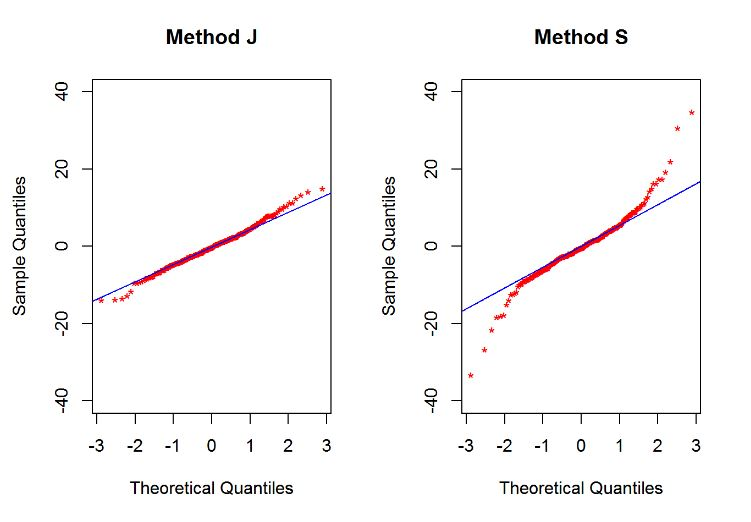
\includegraphics[width=1.1\linewidth]{images/Resid-newplot2}
		\caption{}
		\label{fig:Resid-newplot2}
	\end{figure}
	
	
	\begin{figure}[h!]
		\centering
		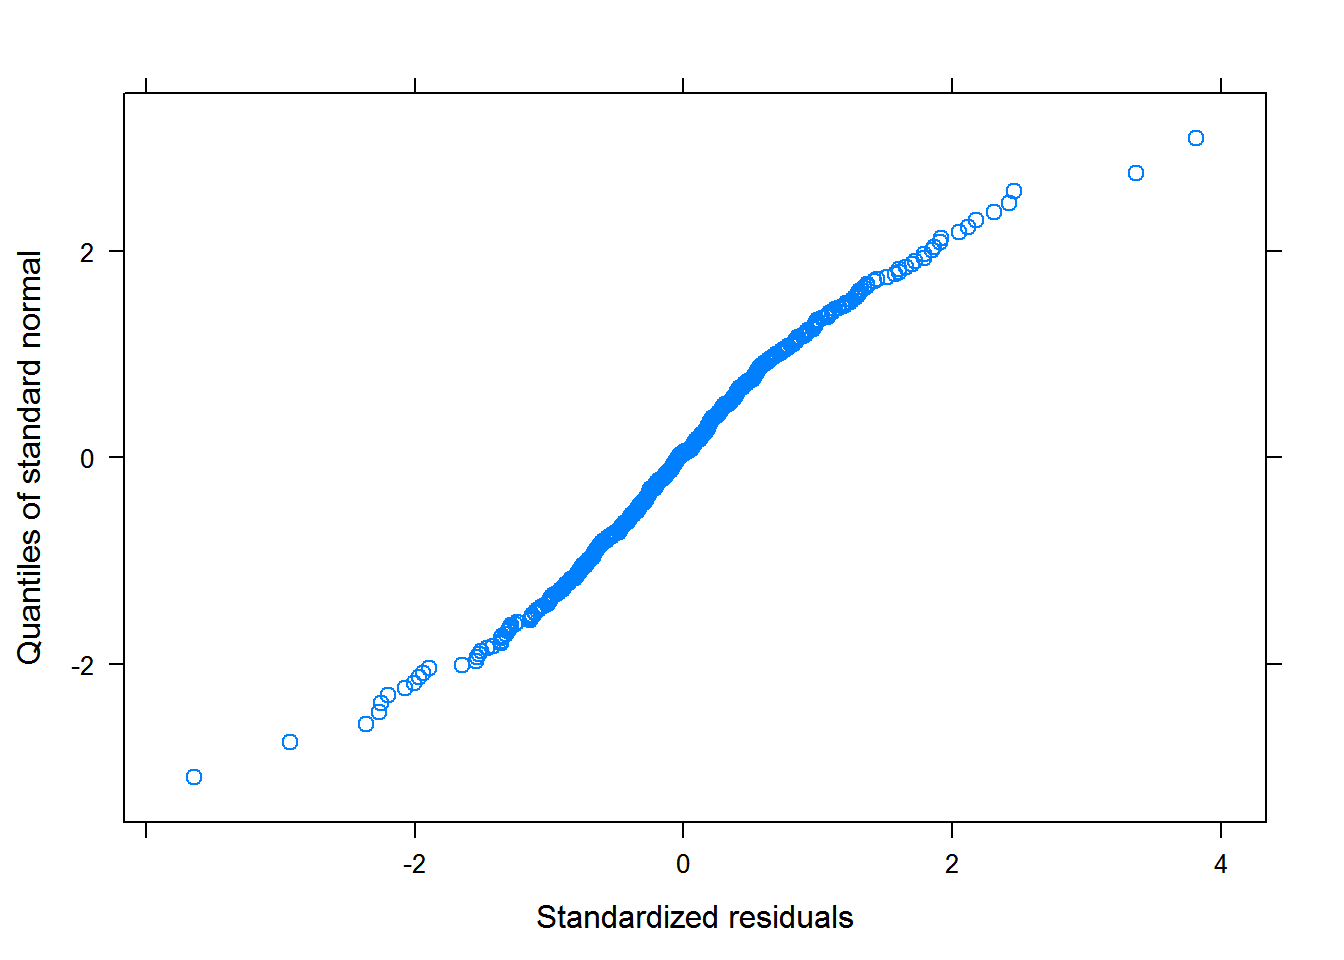
\includegraphics[width=0.9\linewidth]{images/ResidPlot3}
		\label{fig:ResidPlot3}
	\end{figure}
	
	This code will allow you to make QQ plots for each level of the random effects.  LME models assume that not only the within-cluster residuals are normally distributed, but that each level of the random effects are as well. Depending on the model, you can vary the level from 0, 1, 2 and so on
	\begin{framed}
		\begin{verbatim}
		qqnorm(JS.ARoy20091, ~ranef(.))
		
		# 	qqnorm(JS.ARoy20091, ~ranef(.,levels=1)
		\end{verbatim}
	\end{framed}
	\begin{figure}[h!]
		\centering
		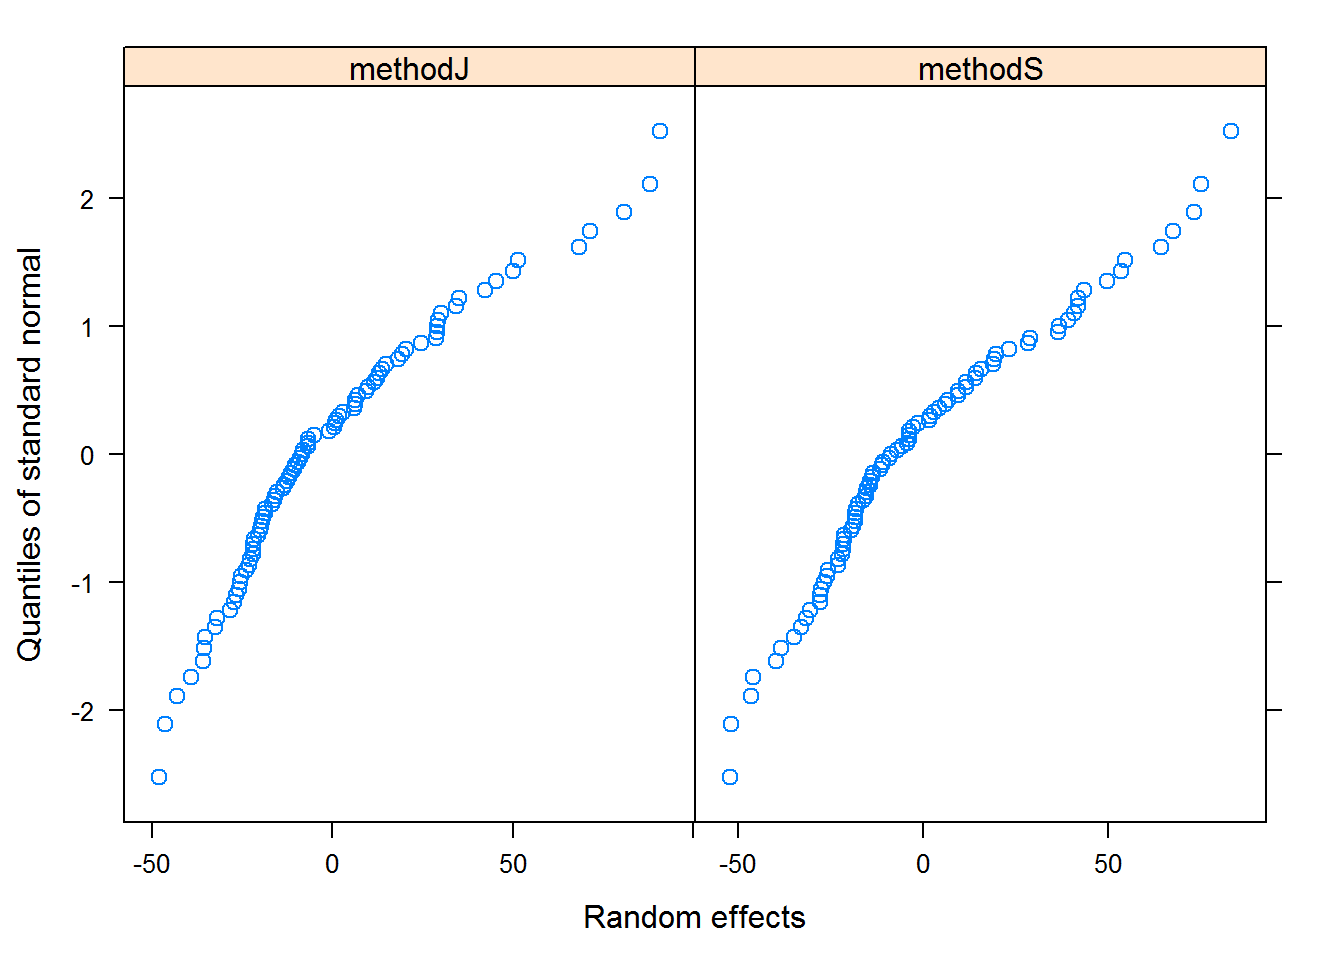
\includegraphics[width=0.9\linewidth]{images/ResidPlot2}
		\caption{}
		\label{fig:ResidPlot2}
	\end{figure}	
	
	\section{Definition of Replicate measurements}
	Further to \citet{BA99}, a formal definition is required of what exactly replicate measurements are
	
	\emph{By replicates we mean two or more measurements on the same
		individual taken in identical conditions. In general this requirement means that the
		measurements are taken in quick succession.}
	
	\citet{BA99} also remark that an important feature of replicate observations is that they should be independent
	of each other. This issue is addressed by \citet{BXC2010}, in terms of exchangeability and linkage. Carstenen advises that repeated measurements come in two \emph{substantially different} forms, depending on the circumstances of their measurement: exchangable and linked.
	%----------------------------------------------------------------------------%
	\subsection{Exchangeable measurements}
	Repeated measurements are said to be exchangeable if no relationship exists between successive measurements across measurements. If the condition of exchangeability exists, a group of measurement of the same item determined by the same method can be re-arranged in any permutation without prejudice to proper analysis. There is no reason to believe that the true value of the underlying variable has changed over the course of the measurements.
	
	For the purposes of method comparison studies the following remarks can be made. The $r-$th measurement made by method $1$ has no special correspondence to the $r-$th measurement made by method $2$, and consequently any pairing of repeated measurements are as good as each other.
	
	Exchangeable repeated measurements can be treated as true replicates.
	%----------------------------------------------------------------------------%
	\subsection{Linked measurements}
	Repeated measurements are said to be linked if a direct correspondence exists between successive measurements across measurements, i.e. pairing. Such measurements are commonly made with a time interval between them, but simultaneously for both methods. Paired measurements are exchangeable, but individual measurements are not.
	
	If the paired measurements are taken
	in a short period of time so that no real systemic changes can take place on each item, they can be considered true replicates.
	Should enough time elapse for systemic changes, linked repeated measurements can not be treated as true replicates.
	
	\subsection{Replicate measurements in ARoy2009's paper}
	\citet{ARoy2009} takes its definition of replicate measurement: two or more measurements on the same item taken
	under identical conditions. ARoy2009 also assumes linked measurements, but it is can be used for the non-linked case.
	
	%----------------------------------------------------------------------------------------------------%
	\newpage
	\subsection{Random effects}
	
	Further to \citet{barnhart}, if the measurements by a method on an item are not necessarily true replications, e.g., repeated measures over time, then additional terms may be needed for $e_{mir}$. \citet{BXC2008} also addresses this issue by the addition of an interaction term (i.e. a random effect) $u_mi$, yielding
	
	\[ y_{mir} =  \alpha_{mi} + u_{mi} + e_{mi}.  \]
	
	The additional interaction term is characterized as $u_{mi}  \sim \mathcal{N}(0, \tau^2_m)$ \citep{BXC2008}.
	
	This extra interaction term provides a source of extra variability, but this variance is not relevant to computing the case-wise differences.
	
	\citet{BXC2008} advises that the formulation of the model should take the exchangeability (in other words, whether or not the measurements are `true replicates') into account. If there is a linkage between measurements (therefore not `true' replicates) , the `item by replicate' should be included in the model. If there is no linkage, and the replicates are indeed true replicates, the interaction term should be omitted.
	
	\citet{BXC2008} demonstrates how to compute the limits of agreement for two methods in the case of linked measurements. As a surplus source of variability is excluded from the computation, the limits of agreement are not unduly wide, which would have been the case if the measurements were treated as true replicates.
	
	\citet{ARoy2009} also assigns a random effect $u_{mi}$ for each response $y_{mir}$. Importantly ARoy2009's model assumes linkage.
	
	%----------------------------------------------------------------------------%
	\section{Model for replicate measurements}
	
	We generalize the single measurement model for the replicate measurement case, by additionally specifying replicate values. Let $y_{mir}$ be the $r-$th replicate measurement for subject ``i" made by method ``m". Further to \citet{barnhart} fixed effect can be expressed with a single term $\alpha_{mi}$, which incorporate the true value $\mu_i$.
	
	\[ y_{mir} = \mu_{i} + \alpha_{m} + e_{mir}  \]
	
	Combining fixed effects \citep{barnhart}, we write,
	
	\[ y_{mir} = \alpha_{mi} + e_{mir}.\]
	
	The following assumptions are required
	
	\begin{itemize}
		\item $e_{mir}$ is independent of the fixed effects with mean $\mbox{E}(e_{mir}) = 0$.
		\item Further to \citet{barnhart} between-item and within-item variances $\mbox{Var}(\alpha_{mi}) = \sigma^2_{Bm}$ and $\mbox{Var}(e_{mir}) = \sigma^2_{Wm}$
		\item In keeping with \citet{ARoy2009}, these variance shall be considered as part of the between-item variance covariance matrix $\boldsymbol{D}$ and the within-item variance covariance matrix  $\boldsymbol{\Sigma}$
		respectively, and will be denoted accordingly ( i.e. $d^2_{m}$ and $\sigma^2_{m}$).
		\item Additionally, the total variability of method "m", denoted $\omega^2_m$ is the sum of the within-item and between-item variabilities.
		
		\[ \omega^2_m = d^2_{m}+ \sigma^2_{m} \]
		
	\end{itemize}
	%----------------------------------------------------------------------------%
	\newpage
	
	
	\chapter{BXC}	
	\section{2004 Model}
	\cite{BXC2004} also advocates the use of linear mixed models in the study of method comparisons. 
	The model is constructed to describe the relationship between a value of measurement and its
	real value.
	The non-replicate case is considered first, as it is the context of the Bland Altman plots. This model assumes that
	inter-method bias is the only difference between the two methods. A measurement $y_{mi}$ by method $m$ on individual $i$ is
	formulated as follows;
	
	\begin{equation}
	y_{mi}  = \alpha_{m} + \mu_{i} + e_{mi} \qquad ( e_{mi} \sim
	N(0,\sigma^{2}_{m}))
	\end{equation}
	
	The differences are expressed as $d_{i} = y_{1i} - y_{2i}$. For the replicate case, an interaction term $c$ is added to the model, with an associated variance component. All the random effects are assumed independent, and that all replicate measurements are assumed to be exchangeable within each method.
	\begin{equation}
	y_{mir}  = \alpha_{m} + \mu_{i} + c_{mi} + e_{mir} \qquad ( e_{mi}
	\sim N(0,\sigma^{2}_{m}), c_{mi} \sim N(0,\tau^{2}_{m}))
	\end{equation}
	\section{Carstensen's Model}
	\cite{BXC2008} also use a LME model for the purpose of comparing two methods of measurement where replicate measurements are available on each item. Their interest lies in generalizing the popular limits-of-agreement (LOA) methodology advocated by \citet{BA86} to take proper cognizance of the replicate measurements. \citet{BXC2008} demonstrate statistical flaws with two approaches proposed by \citet{BA99} for the purpose of calculating the variance of the inter-method bias when replicate measurements are available. Instead, they recommend a fitted mixed effects model to obtain appropriate estimates for the variance of the inter-method bias. As their interest mainly lies in extending the Bland-Altman methodology, other formal tests are not considered.
	
	
	\citet{BXC2008} presents a methodology to compute the limits of
	agreement based on LME models. Importantly, Carstensen's underlying model differs from ARoy2009's model in some key respects, and therefore a prior discussion of Carstensen's model is required. The method of computation is the
	same as ARoy2009's model, but with the covariance estimates set to zero.
	
	In cases where there is negligible covariance between methods, the limits of agreement computed using ARoy2009's model accord with those computed using Carstensen's model. In cases where some degree of
	covariance is present between the two methods, the limits of agreement computed using models will differ. In the presented
	example, it is shown that ARoy2009's LoAs are lower than those of Carstensen, when covariance is present.
	
	Importantly, estimates required to calculate the limits of agreement are not extractable, and therefore the calculation must
	be done by hand.
	%-----------------------------------------------------------------------------------------------------%
	
	
	Bendix Carstensen et al. proposed the use of LME models to allow for a more statistically rigourous approach to computing Limits of Agreement.  The respective papers also discuss several shortcoming for techniques for dealing with replicate measurements, as proposed by Bland-Altman 1999.
	
	
	
	\begin{equation}
	y_{mir}  = \alpha_{m} + \mu_{i} + c_{mi} + e_{mir}, \qquad  e_{mi}
	\sim \mathcal{N}(0,\sigma^{2}_{m}), \quad c_{mi} \sim \mathcal{N}(0,\tau^{2}_{m}).
	\end{equation}
	
	
	The above formulation doesn't require the data set to be balanced.
	However, it does require a sufficient large number of replicates
	and measurements to overcome the problem of identifiability. The
	import of which is that more than two methods of measurement may
	be required to carry out the analysis. There is also the
	assumptions that observations of measurements by particular
	methods are exchangeable within subjects. (Exchangeability means
	that future samples from a population behaves like earlier
	samples).
	
	%\citet{BXC2004} describes the above model as a `functional model',
	%similar to models described by \citet{Kimura}, but without any
	%assumptions on variance ratios. A functional model is . An
	%alternative to functional models is structural modelling
	
	\citet{BXC2004} uses the above formula to predict observations for
	a specific individual $i$ by method $m$;
	
	\begin{equation}BLUP_{mir} = \hat{\alpha_{m}} + \hat{\beta_{m}}\mu_{i} +
	c_{mi} \end{equation}. Under the assumption that the $\mu$s are
	the true item values, this would be sufficient to estimate
	parameters. When that assumption doesn't hold, regression
	techniques (known as updating techniques) can be used additionally
	to determine the estimates. The assumption of exchangeability can
	be unrealistic in certain situations. \citet{BXC2004} provides an
	amended formulation which includes an extra interaction term ($
	d_{mr} \sim N(0,\omega^{2}_{m}$)to account for this.
	
	%======================================================== %
	
	
	\citet{BXC2004} presents a model to describe the relationship between a value of measurement and its
	real value. The non-replicate case is considered first, as it is the context of the Bland Altman plots. This model assumes that inter-method bias is the only difference between the two methods.
	
	
	%----
	
	Of particular importance is terms of the model, a true value for item $i$ ($\mu_{i}$).  The fixed effect of ARoy2009's model comprise of an intercept term and fixed effect terms for both methods, with no reference to the true value of any individual item. A distinction can be made between the two models: ARoy2009's model is a standard LME model, whereas Carstensen's model is a more complex additive model.
	
	
	
	Let $y_{mir} $ denote the $r$th replicate measurement on the $i$th item by the $m$th method, where $m=1,2$ ; $i=1,\ldots,N;$ and $r = 1,\ldots,n_i.$ When the design is balanced and there is no ambiguity we can set $n_i=n.$ The LME model underpinning ARoy2009's approach can be written
	\begin{equation}\label{ARoy2009-model}
	y_{mir} = \beta_{0} + \beta_{m} + b_{mi} + \epsilon_{mir}.
	\end{equation}
	Here $\beta_0$ and $\beta_m$ are fixed-effect terms representing, respectively, a model intercept and an overall effect for method $m.$ The model can be reparameterized by gathering the $\beta$ terms together into (fixed effect) intercept terms $\alpha_m=\beta_0+\beta_m.$ The $b_{1i}$ and $b_{2i}$ terms are correlated random effect parameters having $\mathrm{E}(b_{mi})=0$ with $\mathrm{Var}(b_{mi})=g^2_m$ and $\mathrm{Cov}(b_{1i}, b_{2 i})=g_{12}.$ The random error term for each response is denoted $\epsilon_{mir}$ having $\mathrm{E}(\epsilon_{mir})=0$, $\mathrm{Var}(\epsilon_{mir})=\sigma^2_m$, $\mathrm{Cov}(\epsilon_{1ir}, \epsilon_{2 ir})=\sigma_{12}$, $\mathrm{Cov}(\epsilon_{mir}, \epsilon_{mir^\prime})= 0$ and $\mathrm{Cov}(\epsilon_{1ir}, \epsilon_{2 ir^\prime})= 0.$ Additionally these parameter are assumed to have Gaussian distribution. Two methods of measurement are in complete agreement if the null hypotheses $\mathrm{H}_1\colon \alpha_1 = \alpha_2$ and $\mathrm{H}_2\colon \sigma^2_1 = \sigma^2_2 $ and $\mathrm{H}_3\colon g^2_1= g^2_2$ hold simultaneously. \citet{ARoy2009} uses a Bonferroni correction to control the familywise error rate for tests of $\{\mathrm{H}_1, \mathrm{H}_2, \mathrm{H}_3\}$ and account for difficulties arising due to multiple testing. Additionally, ARoy2009 combines $\mathrm{H}_2$ and $\mathrm{H}_3$ into a single testable hypothesis $\mathrm{H}_4\colon \omega^2_1=\omega^2_2,$ where $\omega^2_m = \sigma^2_m + g^2_m$ represent the overall variability of method $m.$
	%Disagreement in overall variability may be caused by different between-item variabilities, by different within-item variabilities, or by both.
	
	%If the exact cause of disagreement between the two methods is not of interest, then the overall variability test $H_4$ %is an alternative to testing $H_2$ and $H_3$ separately.
	
	\citet{BXC2008} develop their model from a standard two-way analysis of variance model, reformulated for the case of replicate measurements, with random effects terms specified as appropriate.
	Their model can be written as
	%describing $y_{mir} $, again the $r$th replicate measurement on the $i$th item by the $m$th method ($m=1,2,$ %$i=1,\ldots,N,$ and $r = 1,\ldots,n$),
	
	\begin{equation}\label{BXC-model}
	y_{mir}  = \alpha_{m} + \mu_{i} + a_{ir} + c_{mi} + \varepsilon_{mir}.
	\end{equation}
	
	The fixed effects $\alpha_{m}$ and $\mu_{i}$ represent the intercept for method $m$ and the `true value' for item $i$ respectively. The random-effect terms comprise an item-by-replicate interaction term $a_{ir} \sim \mathcal{N}(0,\varsigma^{2})$, a method-by-item interaction term $c_{mi} \sim \mathcal{N}(0,\tau^{2}_{m}),$ and model error terms $\varepsilon_{mir} \sim \mathcal{N}(0,\varphi^{2}_{m}).$ All random-effect terms are assumed to be independent. For the case when replicate measurements are assumed to be exchangeable for item $i$, $a_{ir}$ can be removed. The model expressed in (2) describes measurements by $m$ methods, where $m = \{1,2,3\ldots\}$. Based on the model expressed in (2), \citet{BXC2008} compute the limits of agreement as
	\[
	\alpha_1 - \alpha_2 \pm 2 \sqrt{ \tau^2_1 +  \tau^2_2 +  \varphi^2_1 +  \varphi^2_2 }
	\]
	\citet{BXC2008} notes that, for $m=2$,  separate estimates of $\tau^2_m$ can not be obtained. To overcome this, the assumption of equality, i.e. $\tau^2_1 = \tau^2_2$ is required.
	
	%%---Comparative Complexity
	There is a substantial difference in the number of fixed parameters used by the respective models; the model in (\ref{ARoy2009-model}) requires two fixed effect parameters, i.e. the means of the two methods, for any number of items $N$, whereas the model in (\ref{BXC-model}) requires $N+2$ fixed effects.
	
	Allocating fixed effects to each item $i$ by (\ref{BXC-model}) accords with earlier work on comparing methods of measurement, such as \citet{Grubbs48}. However allocation of fixed effects in ANOVA models suggests that the group of items is itself of particular interest, rather than as a representative sample used of the overall population. However this approach seems contrary to the purpose of LOAs as a prediction interval for a population of items. Conversely, \citet{ARoy2009}
	uses a more intuitive approach, treating the observations as a random sample population, and allocating random effects accordingly.
	
	
	\section{Using Interaction Terms}
	\citet{BXC2008} formulates an LME model, both in the absence and the presence of an interaction term.\citet{BXC} uses both to demonstrate the importance of using an interaction term. Failure to take the replication structure into
	account results in over-estimation of the limits of agreement. For the Carstensen estimates below, an interaction term was included when computed.
	
	
	\section{Computing LoAs with LMEs}
	%\subsection{Carstensen's LOAs}
	
	
	Carstensen presents a model where the variation between items for
	method $m$ is captured by $\sigma_m$ and the within item variation
	by $\tau_m$.
	
	Further to his model, Carstensen computes the limits of agreement
	as
	
	\[
	\hat{\alpha}_1 - \hat{\alpha}_2 \pm \sqrt{2 \hat{\tau}^2 +
		\hat{\sigma}^2_1 + \hat{\sigma}^2_2}
	\]
	
	%---------------------------------------------------------------------------------%
	
	
	
	\section{Carstensen's Model}
	\citet{BXC2004} proposes linear mixed effects models for deriving
	conversion calculations similar to Deming's regression, and for
	estimating variance components for measurements by different
	methods. The following model ( in the authors own notation) is
	formulated as follows, where $y_{mir}$ is the $r$th replicate
	measurement on subject $i$ with method $m$.
	
	\begin{equation}
	y_{mir}  = \alpha_{m} + \beta_{m}\mu_{i} + c_{mi} + e_{mir} \qquad
	( e_{mi} \sim N(0,\sigma^{2}_{m}), c_{mi} \sim N(0,\tau^{2}_{m}))
	\end{equation}
	The intercept term $\alpha$ and the $\beta_{m}\mu_{i}$ term follow
	from \citet{DunnSEME}, expressing constant and proportional bias
	respectively , in the presence of a real value $\mu_{i}.$
	$c_{mi}$ is a interaction term to account for replicate, and
	$e_{mir}$ is the residual associated with each observation.
	Since variances are specific to each method, this model can be
	fitted separately for each method.
	
	The above formulation doesn't require the data set to be balanced.
	However, it does require a sufficient large number of replicates
	and measurements to overcome the problem of identifiability. The
	import of which is that more than two methods of measurement may
	be required to carry out the analysis. There is also the
	assumptions that mobservations of measurements by particular
	methods are exchangeable within subjects. (Exchangeability means
	that future samples from a population behaves like earlier
	samples).
	
	Using Carstensen's notation, a measurement $y_{mi}$ by method $m$ on individual $i$ the measurement $y_{mir} $ is the $r$th replicate measurement on the $i$th item by the $m$th method, where $m=1,2,\ldots,M$ $i=1,\ldots,N,$ and $r = 1,\ldots,n_i$ is formulated as follows;
	\begin{equation}
	y_{mir}  = \alpha_{m} + \mu_{i} + c_{mi} + a_{ir} + \epsilon_{mir}, \qquad \quad c_{mi} \sim \mathcal{N}(0,\tau^{2}_{m}) , a_{ir} \sim \mathcal{N}(0,\varsigma^{2}),  \varepsilon_{mi} \sim \mathcal{N}(0,\varphi^{2}_{m}) .
	\end{equation}
	
	Here the terms $\alpha_{m}$ and $\mu_{i}$ represent the fixed effect for method $m$ and a true value for item $i$ respectively. The random effect terms comprise an interaction term $c_{mi}$ and the residuals $\varepsilon_{mir}$.
	The $c_{mi}$ term represent random effect parameters corresponding to the two methods, having $\mathrm{E}(c_{mi})= 0$ with $\mathrm{Var}(c_{mi})=\tau^2_m$.  
	
	%%%%Stuff about extra interaction term
	
	The random error term for each response is denoted $\varepsilon_{mir}$ having $\mathrm{E}(\varepsilon_{mir})=0$, $\mathrm{Var}(\varepsilon_{mir})=\varphi^2_m$. All the random effects are assumed independent, and that all replicate measurements are assumed to be exchangeable within each method.
	
	%Carstensen specifies the variance of the interaction terms as being univariate normally distributed. As such, $\mathrm{Cov}(c_{mi}, c_{m^\prime i})= 0.$
	
	When only two methods are to be compared, separate estimates of $\tau^2_m$ can not be obtained. Instead the average value $\tau^2$ is obtained and used.
	
	
	Carstensen's approach is that of a standard two-way mixed effects ANOVA with replicate measurements. With regards to the specification of the variance terms, Carstensen remarks that using his approach is common, remarking that \emph{
		The only slightly non-standard (meaning "not often used") feature is the differing residual variances between methods }\citep{BXC2010}.
	
	In contrast to ARoy2009's model, Carstensen's model requires that commonly used assumptions be applied, specifically that the off-diagonal elements of the between-item and within-item variability matrices are zero. By
	extension the overall variability off-diagonal elements are also zero. Also, implementation requires that the between-item variances are estimated as the same value: $\tau^2_1 = \tau^2_2 = \tau^2$.
	Also, implementation requires that the between-item variances are estimated as the same value: $g^2_1 = g^2_2 = g^2$.
	As a consequence, Carstensen's method does not allow for a formal test of the between-item variability.
	
	\[\left(\begin{array}{cc}
	\omega^1_2  & 0 \\
	0 & \omega^2_2 \\
	\end{array}  \right)
	=  \left(
	\begin{array}{cc}
	\tau^2  & 0 \\
	0 & \tau^2 \\
	\end{array} \right)+
	\left(
	\begin{array}{cc}
	\sigma^2_1  & 0 \\
	0 & \sigma^2_2 \\
	\end{array}\right)
	\]
	
	
	\[\left(\begin{array}{cc}
	\omega^1_2  & 0 \\
	0 & \omega^2_2 \\
	\end{array}  \right)
	=  \left(
	\begin{array}{cc}
	\tau^2  & 0 \\
	0 & \tau^2 \\
	\end{array} \right)+
	\left(
	\begin{array}{cc}
	\sigma^2_1  & 0 \\
	0 & \sigma^2_2 \\
	\end{array}\right)
	\]
	
	%---Key difference 1---The True Value
	%---Colollary -- Difference in model types
	The presence of the true value term $\mu_i$ gives rise to an important difference between Carstensen's and ARoy2009's models. The fixed effect of ARoy2009's model comprise of an intercept term and fixed effect terms for both methods, with no reference to the true value of any individual item. In other words, ARoy2009 considers the group of items being measured as a sample taken from a population. Therefore a distinction can be made between the two models: ARoy2009's model is a standard LME model, whereas Carstensen's model is a more complex additive model.
	
	%---Carstensen's limits of agreement
	%---The between item variances are not individually computed. An estimate for their sum is used.
	%---The within item variances are indivdually specified.
	%---Carstensen remarks upon this in his book (page 61), saying that it is "not often used".
	%---The Carstensen model does not include covariance terms for either VC matrices.
	%---Some of Carstensens estimates are presented, but not extractable, from R code, so calculations have to be done by %---hand.
	%---All of ARoy2009s stimates are  extractable from R code, so automatic compuation can be implemented
	%---When there is negligible covariance between the two methods, ARoy2009s LoA and Carstensen's LoA are roughly the same.
	%---When there is covariance between the two methods, ARoy2009's LoA and Carstensen's LoA differ, ARoy2009s usually narrower.
	
	
	\section{Carstensen's Mixed Models}
	
	
	
	\citet{BXC2008} sets out a methodology of computing the limits of
	agreement based upon variance component estimates derived using
	linear mixed effects models. Measures of repeatability, a
	characteristic of individual methods of measurements, are also
	derived using this method.
	
	
	\begin{equation}
	y_{mir}  = \alpha_{m} + \mu_{i} + c_{mi} + e_{mir} \qquad ( e_{mi}
	\sim N(0,\sigma^{2}_{m}), c_{mi} \sim N(0,\tau^{2}_{m}))
	\end{equation}
	
	\citet{BXC2008} proposes a methodology to calculate prediction
	intervals in the presence of replicate measurements, overcoming
	problems associated with Bland-Altman methodology in this regard.
	It is not possible to estimate the interaction variance components
	$\tau^{2}_{1}$ and $\tau^{2}_{2}$ separately. Therefore it must be
	assumed that they are equal. The variance of the difference can be
	estimated as follows:
	\begin{equation}
	var(y_{1j}-y_{2j})
	\end{equation}
	
	
	%-----------------------------------------------------------------------------------------------------%
	
	
	
	\subsection{Carstensen Methods}
	
	%---------------------------------------------------------------%
	Components
	
	\begin{verbatim}
	
	
	
	Section 5.3 Models for replicate measurements
	Section 5 Replicate measurements.
	
	Carstensen page 56
	%----------------------------------------------------------------%
	air extra random effect that does not depend on method.
	It is treated as an extension of i.
	The variance of air represents the variation between replication condition (common for all methods), within items, .
	\end{verbatim}
	\[ymir=m+i+cmi+emir\]
	
	\[cmi=N(0,m2)\]
	
	\[emir=N(0,m2)\]
	
	\begin{verbatim}
	Carstensen page 58
	
	var(y10-y20) =12+22+12+22
	
	1-2222+12+22
	
	ARoy2009 further to Carstensen
	
	ymir=m+i+cmi+emir
	
	\end{verbatim}
	%-----------------------------------------------------------------%
	
	
	Section 7 A general model for method comparisons.
	
	Carstensen discusses the model and its use as if all parameter estimates are available.
	
	In this model, intermethod bias is assumed to be constant at all measurement levels.
	
	i : True value for item i
	
	The parameter i can be thought of as the underlying, but unobtainable, true measurement for item i.
	
	m: Fixed effect for method m
	
	%%-----------------------------------------------------------------%
	%
	%\subsection{7.2 Interpretation of Random effects}
	%
	%
	%	 method by item
	%	 item by replicate
	%	 method by item by replicate
	%
	
	%Carstensen’s LME model
	%LoA as computed by Carstensen’s LME model Papers
	%Carstensen et Al 2006
	%Carstensen et al 2008
	%Bendix Carstensen 2010
	% Section 5.3 Models for replicate measurements
	% Section 7 A general model for method comparisons.
	% Section 7.2 Interpretation of Random effects
	%
	\textbf{Carstensen et al - Mixed Models}
	
	Carstensen et al [4] also advocates the use of linear mixed models in
	the study of method comparisons. The model is constructed to
	describe the relationship between a value of measurement and its
	real value. 
	
	The non-replicate case is considered first, as it is
	the context of the Bland-Altman plots. 
	This model assumes that
	\textit{inter-method bias} is the only difference between the two methods.
	A measurement $y_{mi}$ by method $m$ on individual $i$ is
	formulated as follows;
	
	
	\begin{equation}
	y_{mi}  = \alpha_{m} + \mu_{i} + e_{mi} \qquad ( e_{mi} \sim
	N(0,\sigma^{2}_{m}))
	\end{equation}
	
	%%%%%%%%%%%%%%%%%%%%%%%%%%%%%%%%%%%%%%%%%%%%%%%%%%%%%%%%%%%%%%%%%%%%%%%%%%%%%%%%%%%%%%
	
	%%%%%%%%%%%%%%%%%%%%%%%%%%%%%%%%%%%%%%%%%%%%%%%%%%%%%%%%%%%%%%%%%%%%%%%%%%%%%%%%%%%%%%
	
	%
	% \frametitle{Carstensen's Mixed Models}
	
	Carstensen et al [5] sets out a methodology of computing the limits of
	agreement based upon variance component estimates derived using
	linear mixed effects models. 
	Measures of repeatability, a
	characteristic of individual methods of measurements, are also
	derived using this method.
	
	
	
	%%%%%%%%%%%%%%%%%%%%%%%%%%%%%%%%%%%%%%%%%%%%%%%%%%%%%%%%%%%%%%%%%%%%%%%%%%%%%%%%%%%%%%
	%
	% \frametitle{Carstensen's Mixed Models}
	
	
	The differences are expressed as $d_{i} = y_{1i} - y_{2i}$.
	For the
	replicate case, an interaction term $c$ is added to the model,
	with an associated variance component. 
	All the random effects are
	assumed independent, and that all replicate measurements are
	assumed to be exchangeable within each method.
	
	
	
	\begin{equation}
	y_{mir}  = \alpha_{m} + \mu_{i} + c_{mi} + e_{mir} \qquad ( e_{mi}
	\sim N(0,\sigma^{2}_{m}), c_{mi} \sim N(0,\tau^{2}_{m}))
	\end{equation}
	%%%%%%%%%%%%%%%%%%%%%%%%%%%%%%%%%%%%%%%%%%%%%%%%%%%%%%%%%%%%%%%%%%%%%%%%%%%%%%%%%%%%%%
	
	
	
	Carstensen \textit{et al} \cite{BXC2004} also advocates the use of linear mixed models in
	the study of method comparisons. 
	The model is constructed to
	describe the relationship between a value of measurement and its
	real value.
	The non-replicate case is considered first, as it is
	the context of the Bland Altman plots. This model assumes that
	inter-method bias is the only difference between the two methods.
	A measurement $y_{mi}$ by method $m$ on individual $i$ is
	formulated as follows;
	
	\begin{equation}
	y_{mi}  = \alpha_{m} + \mu_{i} + e_{mi} \qquad ( e_{mi} \sim
	N(0,\sigma^{2}_{m}))
	\end{equation}
	
	
	
	
	The differences are expressed as $d_{i} = y_{1i} - y_{2i}$ For the
	replicate case, an interaction term $c$ is added to the model,
	with an associated variance component. 
	All the random effects are
	assumed independent, and that all replicate measurements are
	assumed to be exchangeable within each method.
	
	\begin{eqnarray}
	y_{mir}  = \alpha_{m} + \mu_{i} + c_{mi} + e_{mir} 
	\end{eqnarray}
	
	%------------------------------------------------------------------------------ %
	
	
	The following model (in the authors own notation) is
	formulated as follows, where $y_{mir}$ is the $r$th replicate
	measurement on subject $i$ with method $m$.
	
	{
		
		\begin{equation}
		y_{mir}  = \alpha_{m} + \mu_{i} + c_{mi} + e_{mir} \qquad ( e_{mi}
		\sim N(0,\sigma^{2}_{m}), c_{mi} \sim N(0,\tau^{2}_{m}))
		\end{equation}
		
		
		\begin{equation}
		y_{mir}  = \alpha_{m} + \beta_{m}\mu_{i} + c_{mi} + e_{mir} 
		\end{equation}
	}
	
	{
		
		\[ e_{mi} \sim N(0,\sigma^{2}_{m}), c_{mi} \sim N(0,\tau^{2}_{m})\]
	}
	
	%------------------------------------------------------- %
	%SLIDE 3
	%[fragile]
	% \frametitle{Carstensen's Mixed Models}
	
	The intercept term $\alpha$ and the $\beta_{m}\mu_{i}$ term follow
	from \textit{Dunn} \cite{DunnSEME}, expressing constant and proportional bias
	respectively , in the presence of a real value $\mu_{i}.$
	$c_{mi}$ is a interaction term to account for replicate, and
	$e_{mir}$ is the residual associated with each observation.
	Since variances are specific to each method, this model can be
	fitted separately for each method.
	
	
	
	%---------------------------------------------------------------- %
	%
	% \frametitle{Carstensen's Mixed Models}
	
	The above formulation doesn't require the data set to be balanced.
	However, it does require a sufficient large number of replicates
	and measurements to overcome the problem of identifiability. 
	The
	import of which is that more than two methods of measurement may
	be required to carry out the analysis. 
	
	There is also the
	assumptions that observations of measurements by particular
	methods are exchangeable within subjects.  \textbf{\textit{Exchangeability}} means
	that future samples from a population behaves like earlier
	samples).
	
	
	%---------------------------------------------------------------- %
	
	%-----------------------%
	%
	% \frametitle{Computing LoAs from LME models}
	\emph{
		One important feature of replicate observations is that they should be independent
		of each other. In essence, this is achieved by ensuring that the observer makes each
		measurement independent of knowledge of the previous value(s). This may be difficult
		to achieve in practice.}
	
	
	\subsection{Tau Identifibaility}
	
	Carstensen presents a model where the variation between items for
	method $m$ is captured by $\sigma_m$ and the within item variation
	by $\tau_m$.
	
	Further to his model, Carstensen computes the limits of agreement
	as
	
	\[
	\hat{\alpha}_1 - \hat{\alpha}_2 \pm \sqrt{2 \hat{\tau}^2 +
		\hat{\sigma}^2_1 + \hat{\sigma}^2_2}
	\]
	
	
	%==================================================================== %
	\citet{BXC2008} proposes a methodology to calculate prediction
	intervals in the presence of replicate measurements, overcoming problems associated with Bland-Altman methodology in this regard.
	It is not possible to estimate the interaction variance components
	$\tau^{2}_{1}$ and $\tau^{2}_{2}$ separately. Therefore it must be
	assumed that they are equal. The variance of the difference can be
	estimated as follows:
	\begin{equation}
	var(y_{1j}-y_{2j})
	\end{equation}
	
	
	\subsection{Computation} Modern software
	packages can be used to fit models accordingly. The best linear
	unbiased predictor (BLUP) for a specific subject $i$ measured with
	method $m$ has the form $BLUP_{mir} = \hat{\alpha_{m}} +
	\hat{\beta_{m}}\mu_{i} + c_{mi}$, under the assumption that the
	$\mu$s are the true item values.
	
	
	
	
	
	%%%%%%%%%%%%%%%%%%%%%%%%%%%%%%%%%%%%%%%%%%%%%%%%%%%%%%%%%%%%%%%%%%%%%%%%%%%%%%%%%%%%%%%%%%%%%%%%%%%%%%%%%5
	
	Maximum likelihood estimation is used to estimate the parameters.
	The REML estimation is not considered since it does not lead to a
	joint distribution of the estimates of fixed effects and random
	effects parameters, upon which the assessment of agreement is
	based.
	
	
	
	\subsection{Carstensen's Mixed Models}
	
	%-----------------------------------------------------------------------------------%
	%
	% \frametitle{Carstensen model in the single measurement case}
	
	Carstensen \textit{et al}[4] presents a model to describe the relationship between a value of measurement and its real value.
	The non-replicate case is considered first, as it is the context of the Bland-Altman plots.
	This model assumes that inter-method bias is the only difference between the two methods.
	% Cut This Slide?
	
	Carstensen \textit{et al}[4] proposes linear mixed effects models for deriving
	conversion calculations similar to Deming's regression, and for
	estimating variance components for measurements by different
	methods. The following model ( in the authors own notation) is
	formulated as follows, where $y_{mir}$ is the $r$th replicate
	measurement on subject $i$ with method $m$.
	
	\begin{equation}
	y_{mir}  = \alpha_{m} + \beta_{m}\mu_{i} + c_{mi} + e_{mir} \qquad
	( e_{mi} \sim N(0,\sigma^{2}_{m}), c_{mi} \sim N(0,\tau^{2}_{m}))
	\end{equation}
	
	%%%%%%%%%%%%%%%%%%%%%%%%%%%%%%%%%%%%%%%%%%%%%%%%%%%%%%%%%%%%%%%%%%%%%%%%%%%%%%%%%%%%%%
	%
	The intercept term $\alpha$ and the $\beta_{m}\mu_{i}$ term follow
	from Dunn[7], expressing constant and proportional bias
	respectively , in the presence of a real value $\mu_{i}.$
	$c_{mi}$ is a interaction term to account for replicate, and
	$e_{mir}$ is the residual associated with each observation.
	Since variances are specific to each method, this model can be
	fitted separately for each method.
	
	%-----------------------------------------------------------------------%
	%
	% \frametitle{Carstensen's Mixed Models}
	
	This model includes a method by item interaction term.\\
	
	Carstensen presents two models. One for the case where the replicates, and a second for when they are linked.\\
	Carstensen's model does not take into account either between-item or within-item covariance between methods.\\
	In the presented example, it is shown that ARoy2009's LoAs are lower than those of Carstensen.
	
	
	
	
	\[\left(\begin{array}{cc}
	\omega^1_2  & 0 \\
	0 & \omega^2_2 \\
	\end{array}  \right)
	=  \left(
	\begin{array}{cc}
	\tau^2  & 0 \\
	0 & \tau^2 \\
	\end{array} \right)+
	\left(
	\begin{array}{cc}
	\sigma^2_1  & 0 \\
	0 & \sigma^2_2 \\
	\end{array}\right)
	\]
	
	
	
	
	
	
	
	
	
	%-----------------------------------------------------------------------------------%
	%
	% \frametitle{Carstensen model in the single measurement case}
	
	
	%-------------------------------------------------------------------------------------%
	\subsection{Computing LoAs from LME models}
	
	
	One important feature of replicate observations is that they should be independent
	of each other. In essence, this is achieved by ensuring that the observer makes each
	measurement independent of knowledge of the previous value(s). This may be difficult
	to achieve in practice.
	
	
	
	
	%-------------------------------------------------------------------------------------%
	
	
	
	The respective estimates computed by both methods are tabulated as follows. Evidently there is close correspondence between both sets of estimates.
	
	\citet{BXC2008} formulates an LME model, both in the absence and the presence of an interaction term.\citet{BXC2008} uses both to demonstrate the importance of using an interaction term. Failure to take the replication structure into
	account results in over-estimation of the limits of agreement. 
	For the Carstensen estimates below, an interaction term was included when computed.
	
	
	
	
	Using Carstensen's notation, a measurement $y_{mi}$ by method $m$ on individual $i$ the measurement $y_{mir} $ is the $r$th replicate measurement on the $i$th item by the $m$th method, where $m=1,2,$ $i=1,\ldots,N,$ and $r = 1,\ldots,n_i$ is formulated as follows;
	
	\begin{equation}
	y_{mir}  = \alpha_{m} + \mu_{i} + c_{mi} + \epsilon_{mir}, \qquad  e_{mi}
	\sim \mathcal{N}(0,\sigma^{2}_{m}), \quad c_{mi} \sim \mathcal{N}(0,\tau^{2}_{m}).
	\end{equation}
	
	Here the terms $\alpha_{m}$ and $\mu_{i}$ represent the fixed effect for method $m$ and a true value for item $i$ respectively. The random effect terms comprise an interaction term $c_{mi}$ and the residuals $\epsilon_{mir}$.
	The $c_{mi}$ term represent random effect parameters corresponding to the two methods, having $\mathrm{E}(c_{mi})=0$ with $\mathrm{Var}(c_{mi})=\tau^2_m$. Carstensen specifies the variance of the interaction terms as being univariate normally distributed. As such, $\mathrm{Cov}(c_{mi}, c_{m^\prime i})= 0.$ All the random effects are assumed independent, and that all replicate measurements are assumed to be exchangeable within each method.
	
	With regards to specifying the variance terms, Carstensen remarks that using his approach is common, remarking that \emph{
		The only slightly non-standard (meaning "not often used") feature is the differing residual variances between methods }\citep{BXC2010}.
	
	
	
	%---Key difference 1---The True Value
	%---Colollary -- Difference in model types
	The presence of the true value term $\mu_i$ gives rise to an important difference between Carstensen's and ARoy2009's models. The fixed effect of ARoy2009's model comprise of an intercept term and fixed effect terms for both methods, with no reference to the true value of any individual item. In other words, ARoy2009 considers the group of items being measured as a sample taken from a population. Therefore a distinction can be made between the two models: ARoy2009's model is a standard LME model, whereas Carstensen's model is a more complex additive model.
	
	%---Carstensen's limits of agreement
	%---The between item variances are not individually computed. An estimate for their sum is used.
	%---The within item variances are indivdually specified.
	%---Carstensen remarks upon this in his book (page 61), saying that it is "not often used".
	%---The Carstensen model does not include covariance terms for either VC matrices.
	%---Some of Carstensens estimates are presented, but not extractable, from R code, so calculations have to be done by %---hand.
	%---All of ARoy2009s stimates are  extractable from R code, so automatic compuation can be implemented
	%---When there is negligible covariance between the two methods, ARoy2009s LoA and Carstensen's LoA are roughly the same.
	%---When there is covariance between the two methods, ARoy2009's LoA and Carstensen's LoA differ, ARoy2009s usually narrower.
	
	\section{Carstensen 2004 's Mixed Models}
	
	
	%\citet{BXC2004} describes the above model as a `functional model',
	%similar to models described by \citet{Kimura}, but without any
	%assumptions on variance ratios. A functional model is . An
	%alternative to functional models is structural modelling
	
	\citet{BXC2004} uses the above formula to predict observations for
	a specific individual $i$ by method $m$;
	
	\begin{equation}BLUP_{mir} = \hat{\alpha_{m}} + \hat{\beta_{m}}\mu_{i} +
	c_{mi} \end{equation}. Under the assumption that the $\mu$s are
	the true item values, this would be sufficient to estimate
	parameters. When that assumption doesn't hold, regression techniques (known as updating techniques)
	can be used additionally to determine the estimates.
	The assumption of exchangeability can be unrealistic in certain situations.
	\citet{BXC2004} provides an amended formulation which includes an extra interaction
	term ($d_{mr} d_{mr} \sim N(0,\omega^{2}_{m}$)to account for this.
	
	\citet{BXC2008} sets out a methodology of computing the limits of
	agreement based upon variance component estimates derived using
	linear mixed effects models. Measures of repeatability, a
	characteristic of individual methods of measurements, are also
	derived using this method.
	
	
	
	\chapter{BXC Limits of Agreement}
	
	
	%=================================================================================== %
	
	
	\section{Intervals}
	
	\subsection{Purpose of Limits of Agreement} It must be established
	clearly the specific purpose of the limits of agreement.
	\citet*{BA95} comment that the limits of agreement \emph{how far
		apart measurements by the two methods were likely to be for most
		individuals.}, a definition echoed in their 1999 paper:
	\begin{quote} We can then say that nearly all pairs
		of measurements by the two methods will be closer together than
		these extreme values, which we call 95\% limits of agreement.
		These values define the range within which most differences
		between measurements by the two methods will lie\citep{BA99}.
	\end{quote}
	\citet{BXC} offers an alternative, more specific,  definition of
	the limits of agreement \emph{"a prediction interval for the
		difference between future measurements with the two methods on a
		new individual."} \citet{luiz} describes them as tolerance limits.
	
	Importantly they have the same construction as Shewhart Control
	limits.
	
	
	
	\chapter{BXC materials}
	
	
	
	\section{Bendix Carstensen's data sets}
	\citet{BXC2008} describes the sampling method when discussing of a motivating example. Diabetes patients attending an outpatient clinic in Denmark have their $HbA_{1c}$ levels routinely measured at every visit. Venous and Capillary blood samples were obtained from all patients appearing at the clinic over two days. Samples were measured on four consecutive days on each machines, hence there are five analysis days.
	
	\citet{BXC2008} notes that every machine was calibrated every day to  the manufacturers guidelines.
	
	Carstensen notes that every machine was calibrated every day to  the manufacturers guidelines.
	
	Measurements are classified by method, individual and replicate. In this case the replicates are clearly not exchangeable, neither within patients nor simulataneously for all patients.
	
	
	\subsection{Limits of agreement for Carstensen's data}
	
	
	Carstensen demonstrates the use of the interaction term when computing the limits of agreement for the `Oximetry' data set. When the interaction term is omitted, the limits of agreement are $(-9.97, 14.81)$. Carstensen advises the inclusion of the interaction term for linked replicates, and hence the limits of agreement are recomputed as $(-12.18,17.12)$.
	
	
	\subsection{Using LME models to create Prediction Intervals}
	
	
	
	\begin{equation}
	y_{mi}  = \alpha_{m} + \mu_{i} + e_{mi} \qquad ( e_{mi} \sim
	N(0,\sigma^{2}_{m}))
	\end{equation}
	
	%%%%%%%%%%%%%%%%%%%%%%%%%%%%%%%%%%%%%%%%%%%%%%%%%%%%%%%%%%%%%%%%%%%%%%%%%%%%%%%%%%%%%%
	
	%%%%%%%%%%%%%%%%%%%%%%%%%%%%%%%%%%%%%%%%%%%%%%%%%%%%%%%%%%%%%%%%%%%%%%%%%%%%%%%%%%%%%%
	
	
	
	The differences are expressed as $d_{i} = y_{1i} - y_{2i}$.
	For the
	replicate case, an interaction term $c$ is added to the model,
	with an associated variance component. 
	All the random effects are
	assumed independent, and that all replicate measurements are
	assumed to be exchangeable within each method.
	
	
	
	\begin{equation}
	y_{mir}  = \alpha_{m} + \mu_{i} + c_{mi} + e_{mir} \qquad ( e_{mi}
	\sim N(0,\sigma^{2}_{m}), c_{mi} \sim N(0,\tau^{2}_{m}))
	\end{equation}
	%%%%%%%%%%%%%%%%%%%%%%%%%%%%%%%%%%%%%%%%%%%%%%%%%%%%%%%%%%%%%%%%%%%%%%%%%%%%%%%%%%%%%%
	
	
	%%%%%%%%%%%%%%%%%%%%%%%%%%%%%%%%%%%%%%%%%%%%%%%%%%%%%%%%%%%%%%%%%%%%%%%%%%%%%%%%%%%%%%
	%
	
	
	
	%
	
	
	%------------------------------------------------------------------------------ %
	%
	
	
	
	The following model (in the authors own notation) is
	formulated as follows, where $y_{mir}$ is the $r$th replicate
	measurement on subject $i$ with method $m$.
	
	{
		
		\begin{equation}
		y_{mir}  = \alpha_{m} + \mu_{i} + c_{mi} + e_{mir} \qquad ( e_{mi}
		\sim N(0,\sigma^{2}_{m}), c_{mi} \sim N(0,\tau^{2}_{m}))
		\end{equation}
		
		
		\begin{equation}
		y_{mir}  = \alpha_{m} + \beta_{m}\mu_{i} + c_{mi} + e_{mir} 
		\end{equation}
		
		\[ e_{mi} \sim N(0,\sigma^{2}_{m}), c_{mi} \sim N(0,\tau^{2}_{m})\]
	}
	
	
	The
	import of which is that more than two methods of measurement may
	be required to carry out the analysis. 
	
	There is also the
	assumptions that observations of measurements by particular
	methods are exchangeable within subjects.  \textbf{\textit{Exchangeability}} means
	that future samples from a population behaves like earlier
	samples).
	
	
	%---------------------------------------------------------------- %
	
	
	
	
	
	
	
	
	
	\subsection{Carstensen's LOAs}
	%
	Carstensen presents a model where the variation between items for
	method $m$ is captured by $\sigma_m$ and the within item variation
	by $\tau_m$.
	
	Further to his model, Carstensen computes the limits of agreement
	as
	
	\[
	\hat{\alpha}_1 - \hat{\alpha}_2 \pm \sqrt{2 \hat{\tau}^2 +
		\hat{\sigma}^2_1 + \hat{\sigma}^2_2}
	\]
	
	%-------------------------------------------------------------------------------------%
	%
	% \frametitle{Carstensen's LOAs}
	
	
	The respective estimates computed by both methods are tabulated as follows. Evidently there is close correspondence between both sets of estimates.
	
	BXC2008 formulates an LME model, both in the absence and the presence of an interaction term. BXC2008 uses both to demonstrate the importance of using an interaction term. Failure to take the replication structure into
	account results in over-estimation of the limits of agreement. 
	For the Carstensen estimates below, an interaction term was included when computed.
	
	
	
	
	
	%-----------------------------------------------------------------------------------------------------%
	
	\section{The Fat Data Set}
	
	\citet{BXC2008} presents a data set `fat', which is a comparison of measurements of subcutaneous fat
	by two observers at the Steno Diabetes Center, Copenhagen. Measurements are in millimeters
	(mm). Each person is measured three times by each observer. The observations are considered to be `true' replicates.
	
	
	A linear mixed effects model is formulated, and implementation through several software packages is demonstrated.
	All of the necessary terms are presented in the computer output. The limits of agreement are therefore,
	\begin{equation}
	0.0449  \pm 1.96 \times  \sqrt{2 \times 0.0596^2 + 0.0772^2 + 0.0724^2} = (-0.220,  0.309).
	\end{equation}
	
	All of these terms are given or determinable in computer output. The limits of agreement can therefore be evaluated using
	\begin{equation}
	\bar{y_{A}}-\bar{y_{B}} \pm 1.96 \times \sqrt{ \sigma^2_{A} + \sigma^2_{B}  - 2(\sigma_{AB})}.
	\end{equation}
	
	
	
	\citet{AARoy20092009} has demonstrated a methodology whereby $d^2_{A}$ and $d^2_{B}$ can be estimated separately. Also covariance terms are present in both $\boldsymbol{D}$ and $\boldsymbol{\Lambda}$. Using ARoy2009's methodology, the variance of the differences is
	\begin{equation}
	\mbox{var} (y_{iA}-y_{iB})= d^2_{A} + \lambda^2_{B} + d^2_{A} + \lambda^2_{B} - 2(d_{AB} + \lambda_{AB})
	\end{equation}
	
	
	%===========================================================%
	
	
	\citet{BXC2008} describes the calculation of the limits of agreement (with the inter-method bias implicit) for both data sets, based on his formulation;
	
	\[\hat{\alpha}_1 - \hat{\alpha}_2 \pm 2\sqrt{2\hat{\tau}^2 +\hat{\sigma}_1^2 +\hat{\sigma}_2^2 }.\]
	
	
	For the `Fat' data set, the inter-method bias is shown to be $0.045$. The limits of agreement are $(-0.23 , 0.32)$
	
	For Carstensen's `fat' data, the limits of agreement computed using ARoy2009's
	method are consistent with the estimates given by \citet{BXC2008}; $0.044884  \pm 1.96 \times  0.1373979 = (-0.224,  0.314).$
	
	
	
	For Carstensen's `fat' data, the limits of agreement computed using ARoy2009's
	method are consistent with the estimates given by \citet{BXC2008}; $0.044884  \pm 1.96 \times  0.1373979 = (-0.224,  0.314).$
	
	
	
	
	\subsection{Limits of agreement for Carstensen's data}
	
	
	\citet{BXC2008} describes the calculation of the limits of agreement (with the inter-method bias implicit) for both data sets, based on his formulation;
	
	\[\hat{\alpha}_1 - \hat{\alpha}_2 \pm 2\sqrt{2\hat{\tau}^2 +\hat{\sigma}_1^2 +\hat{\sigma}_2^2 }.\]
	
	For the `Fat' data set, the inter-method bias is shown to be $0.045$. The limits of agreement are $(-0.23 , 0.32)$
	
	
	
	%=========================================================================== %
	\section{Oxymetry Data}
	\citet{BXC2008} proposes the addition of an random effects term to their model when the replicates are linked. This term is used to describe the `\textit{item by replicate}' interaction, which is independent of the methods. This interaction is a source of variability independent of the methods. Therefore failure to account for it will result in variability being wrongly attributed to the methods.
	
	\citet{BXC2008} introduces a second data set; the oximetry study. This study done at the ARoy2009al Children�s Hospital in
	Melbourne to assess the agreement between co-oximetry and pulse oximetry in small babies.
	
	In most cases, measurements were taken by both method at three different times. In some cases there are either one or two pairs of measurements, hence the data is unbalanced. \citet{BXC2008} describes many of the children as being very sick, and with very low oxygen saturations levels. Therefore it must be assumed that a biological change can occur in interim periods, and measurements are not true replicates.
	
	\citet{BXC2008} proposes the addition of an random effects term to their model when the replicates are linked. This term is used to describe the `item by replicate' interaction, which is independent of the methods. This interaction is a source of variability independent of the methods. Therefore failure to account for it will result in variability being wrongly attributed to the methods.
	
	
	\citet{BXC2008} demonstrate the necessity of accounting for linked replicated by comparing the limits of agreement from the `oximetry' data set using a model with the additional term, and one without. When the interaction is accounted for the limits of agreement are (-9.62,14.56). When the interaction is not accounted for, the limits of agreement are (-11.88,16.83). It is shown that the failure to include this additional term results in an over-estimation of the standard deviations of differences.
	
	
	\citet{BXC2008} demonstrates the use of the interaction term when computing the limits of agreement for the `Oximetry' data set. When the interaction term is omitted, the limits of agreement are $(-9.97, 14.81)$. Carstensen advises the inclusion of the interaction term for linked replicates, and hence the limits of agreement are recomputed as $(-12.18,17.12)$.
	
	
	Limits of agreement are determined using ARoy2009's methodology, without adding any additional terms, are found to be consistent with the `interaction' model; $(-9.562, 14.504 )$. ARoy2009's methodology assumes that replicates are linked. However, following Carstensen's example, an addition interaction term is added to the implementation of ARoy2009's model to assess the effect, the limits of agreement estimates do not change. However there is a conspicuous difference in within-subject matrices of ARoy2009's model and the modified model (denoted $1$ and $2$ respectively);
	\begin{equation}
	\hat{\boldsymbol{\Lambda}}_{1}= \left(\begin{array}{cc}
	16.61 &	11.67\\
	11.67 & 27.65 \end{array}\right) \qquad
	\boldsymbol{\hat{\Lambda}}_{2}= \left( \begin{array}{cc}
	7.55 & 2.60 \\
	2.60 & 18.59 \end{array} \right).
	\end{equation}
	
	\noindent (The variance of the additional random effect in model $2$ is $3.01$.)
	
	\citet{akaike} introduces the Akaike information criterion ($AIC$), a model
	selection tool based on the likelihood function. Given a data set, candidate models
	are ranked according to their AIC values, with the model having the lowest AIC being considered the best fit.Two candidate models can said to be equally good if there is a difference of less than $2$ in their AIC values.
	
	The Akaike information criterion (AIC) for both models are $AIC_{1} = 2304.226$ and $AIC_{2} = 2306.226$ , indicating little difference in models. The AIC values for the Carstensen `unlinked' and `linked' models are $1994.66$ and $1955.48$ respectively, indicating an improvement by adding the interaction term.
	
	The $\boldsymbol{\hat{\Lambda}}$ matrices are informative as to the difference between Carstensen's unlinked and linked models. For the oximetry data, the covariance terms (given above as 11.67 and 2.6 respectively ) are of similar magnitudes to the variance terms. Conversely for the `fat' data the covariance term ($-0.00032$) is negligible. When the interaction term is added to the model, the covariance term remains negligible. (For the `fat' data, the difference in AIC values is also approximately $2$).
	
	To conclude, Carstensen's models provided a rigorous way to determine limits of agreement, but don't provide for the computation of $\boldsymbol{\hat{D}}$ and $\boldsymbol{\hat{\Lambda}}$. Therefore the test's proposed by \citet{ARoy2009} can not be implemented. Conversely, accurate limits of agreement as determined by Carstensen's model may also be found using ARoy2009's method. Addition of the interaction term erodes the capability of ARoy2009's methodology to compare candidate models, and therefore shall not be adopted.
	
	Finally, to complement the blood pressure (i.e.`J vs S') method comparison from the previous section (i.e.`J vs S'), the limits of agreement are $15.62 \pm 1.96 \times 20.33 = (-24.22, 55.46)$.)
	
	
	%========================================================== %
	
	
	
	
	
	
	
	\section{RV-IV}
	For the the RV-IC comparison, $\hat{D}$ is given by
	
	
	\begin{equation}
	\hat{D}= \left[ \begin{array}{cc}
	1.6323 & 1.1427  \\
	1.1427 & 1.4498 \\
	\end{array} \right]
	\end{equation}
	
	The estimate for the within-subject variance covariance matrix is
	given by
	\begin{equation}
	\hat{\Sigma}= \left[ \begin{array}{cc}
	0.1072 & 0.0372  \\
	0.0372 & 0.1379  \\
	\end{array}\right]
	\end{equation}
	The estimated overall variance covariance matrix for the the 'RV
	vs IC' comparison is given by
	\begin{equation}
	Block \Omega_{i}= \left[ \begin{array}{cc}
	1.7396 & 1.1799  \\
	1.1799 & 1.5877  \\
	\end{array} \right].
	\end{equation}
	
	The power of the likelihood ratio test may depends on specific sample size and the
	specific number of  replications, and the author proposes simulation studies to examine this further.
	
	
	%--------------------------------------------------------------%
	\chapter{ARoy2009 Testing}
	
	
	\section{Introduction}
	
	\citet{AARoy20092009} uses an approach based on linear mixed effects (LME) models for the purpose of comparing the agreement between two methods of measurement, where replicate measurements on items, typically individuals, by both methods are available. She provides three tests of hypothesis appropriate for evaluating the agreement between the two methods of measurement under this sampling scheme. These tests consider null hypotheses that assume: absence of inter-method bias; equality of between-subject variabilities of the two methods; equality of within-subject variabilities of the two methods. By inter-method bias we mean that a systematic difference exists between observations recorded by the two methods. Differences in between-subject variabilities of the two methods arise when one method is yielding average response levels for individuals than are more variable than the average response levels for the same sample of individuals taken by the other method.  Differences in within-subject variabilities of the two methods arise when one method is yielding responses for an individual than are more variable than the responses for this same individual taken by the other method. The two methods of measurement can be considered to agree, and subsequently can be used interchangeably, if all three null hypotheses are true.
	
	\subsection{Model Specification}
	Let $y_{mir} $ be the $r$th replicate measurement on the $i$th item by the $m$th method, where $m=1,2,$ $i=1,\ldots,N,$ and $r = 1,\ldots,n_i.$ When the design is balanced and there is no ambiguity we can set $n_i=n.$ The LME model can be written
	\begin{equation}
	y_{mir} = \beta_{0} + \beta_{m} + b_{mi} + \epsilon_{mir}.
	\end{equation}
	Here $\beta_0$ and $\beta_m$ are fixed-effect terms representing, respectively, a model intercept and an overall effect for method $m.$ The $b_{1i}$ and $b_{2i}$ terms represent random effect parameters corresponding to the two methods, having $\mathrm{E}(b_{mi})=0$ with $\mathrm{Var}(b_{mi})=g^2_m$ and $\mathrm{Cov}(b_{mi}, b_{m^\prime i})=g_{12}.$ The random error term for each response is denoted $\epsilon_{mir}$ having $\mathrm{E}(\epsilon_{mir})=0$, $\mathrm{Var}(\epsilon_{mir})=\sigma^2_m$, $\mathrm{Cov}(b_{mir}, b_{m^\prime ir})=\sigma_{12}$, $\mathrm{Cov}(\epsilon_{mir}, \epsilon_{mir^\prime})= 0$ and $\mathrm{Cov}(\epsilon_{mir}, \epsilon_{m^\prime ir^\prime})= 0.$
	When two methods of measurement are in agreement, there is no significant differences between $\beta_1$ and $\beta_2,$ $g^2_1 $ and$ g^2_2$, and $\sigma^2_1 $ and$ \sigma^2_2$.
	\bigskip
	
	% Complete paragraph by specifying variances and covariances for epsilons.
	% I thing that these are your sigmas?
	% Also, state equality of the parameters in this model when each of the three hypotheses above are true.
	
	
	\newpage
	
	\section{ARoy2009's Hypotheses Tests}
	
	In order to express ARoy2009's LME model in matrix notation we gather all $2n_i$ observations specific to item $i$ into a single vector  $\boldsymbol{y}_{i} = (y_{1i1},y_{2i1},y_{1i2},\ldots,y_{mir},\ldots,y_{1in_{i}},y_{2in_{i}})^\prime.$ The LME model can be written
	\[
	\boldsymbol{y_{i}} = \boldsymbol{X_{i}\beta} + \boldsymbol{Z_{i}b_{i}} + \boldsymbol{\epsilon_{i}},
	\]
	where $\boldsymbol{\beta}=(\beta_0,\beta_1,\beta_2)^\prime$ is a vector of fixed effects, and $\boldsymbol{X}_i$ is a corresponding $2n_i\times 3$ design matrix for the fixed effects. The random effects are expressed in the vector $\boldsymbol{b}=(b_1,b_2)^\prime$, with $\boldsymbol{Z}_i$ the corresponding $2n_i\times 2$ design matrix. The vector $\boldsymbol{\epsilon}_i$ is a $2n_i\times 1$ vector of residual terms.
	
	It is assumed that $\boldsymbol{b}_i \sim N(0,\boldsymbol{G})$, $\boldsymbol{\epsilon}_i$ is a matrix of random errors distributed as $N(0,\boldsymbol{R}_i)$ and that the random effects and residuals are independent of each other.
	% Assumptions made on the structures of $\boldsymbol{G}$ and $\boldsymbol{R}_i$ will be discussed in due course.
	
	% \texttt{finish}
	
	$\boldsymbol{G}$ is the variance covariance matrix for the random effects $\boldsymbol{b}$.
	i.e. between-item sources of variation. The between-item variance covariance matrix $\boldsymbol{G}$ is constructed as follows:
	
	\[ \mbox{Var}  \left[
	\begin{array}{c}
	b_1   \\
	b_2  \\
	\end{array}
	\right] =  \boldsymbol{G} =\left(
	\begin{array}{cc}
	g^2_1  & g_{12} \\
	g_{12} & g^2_2 \\
	\end{array}
	\right) \]
	It is important to note that no special assumptions about the structure of $\boldsymbol{G}$ are made. An example of such an assumption would be that $\boldsymbol{G}$ is the product of a scalar value and the identity matrix.
	
	$\boldsymbol{R}_{i}$ is the variance covariance matrix for the residuals, i.e. the within-item sources of variation between both methods. Computational analysis of linear mixed effects models allow for the explicit analysis of both $\boldsymbol{G}$ and $\boldsymbol{R_i}$.
	
	\citet{hamlett} shows that $\boldsymbol{R}_{i}$  can be expressed as $\boldsymbol{R}_{i} = \boldsymbol{I}_{n_{i}} \otimes \boldsymbol{\Sigma}$. The partial within-item variance?covariance matrix of two methods at any replicate is denoted $\boldsymbol{\Sigma}$, where $\sigma^2_{1}$ and $\sigma^2_{2}$ are the within-subject variances of the respective methods, and $\sigma_{12}$ is the within-item covariance between the two methods. It is assumed that the within-item variance?covariance matrix $\boldsymbol{\Sigma}$ is the same for all replications. Again it is important to note that no special assumptions are made about the structure of the matrix.
	
	\begin{equation}
	\boldsymbol{\Sigma} = \left( \begin{array}{cc}
	\sigma^2_{1} & \sigma_{12} \\
	\sigma_{12} & \sigma^2_{2} \\
	\end{array}\right)
	\end{equation}
	
	\vspace{1in}
	
	For expository purposes consider the case where each item provides three replicates by each method. Then in matrix notation the model has the structure
	\begin{equation}
	\boldsymbol{y}_{i} =
	\left(
	\begin{array}{ccc}
	1 & 1 & 0 \\
	1 & 0 & 1 \\
	1 & 1 & 0 \\
	1 & 0 & 1 \\
	1 & 1 & 0 \\
	1 & 0 & 1 \\
	\end{array}
	\right)
	\left(
	\begin{array}{c}         \beta_0 \\ \beta_1 \\ \beta_2 \\
	\end{array}
	\right)
	+  \left(
	\begin{array}{cc}
	1 & 0 \\
	0 & 1 \\
	1 & 0 \\
	0 & 1 \\
	1 & 0 \\
	0 & 1 \\
	\end{array}
	\right)\left(
	\begin{array}{c}
	b_{1i} \\   b_{2i} \\
	\end{array}
	\right)
	+
	\left(
	\begin{array}{c}
	\epsilon_{1i1} \\
	\epsilon_{2i1} \\
	\epsilon_{1i2} \\
	\epsilon_{2i2} \\
	\epsilon_{1i3} \\
	\epsilon_{2i3} \\
	\end{array}
	\right) ,
	\end{equation}
	where
	\[
	\boldsymbol{G} =
	\]
	and
	\[
	\boldsymbol{R}_i =
	\]
	
	It is assumed that $\boldsymbol{b}_i \sim N(0,\boldsymbol{G})$,
	$\boldsymbol{\epsilon}_i$ is a matrix of random errors distributed as $N(0,\boldsymbol{R}_i)$ and
	that the random effects and residuals are independent of each other. Assumptions made on the structures of $\boldsymbol{G}$ and $\boldsymbol{R}_i$ will be discussed in due course.
	
	\newpage
	
	
	
	
	
	The overall variability between
	the two methods is the sum of between-item variability
	$\boldsymbol{G}$ and within-item variability
	$\boldsymbol{\Sigma}$. \citet{ARoy2009} denotes the overall variability
	as ${\mbox{Block - }\boldsymbol \Omega_{i}}$. The overall
	variation for methods $1$ and $2$ are given by
	
	\begin{center}
		\[\left(\begin{array}{cc}
		\omega^2_1  & \omega_{12} \\
		\omega_{12} & \omega^2_2 \\
		\end{array}  \right)
		=  \left(
		\begin{array}{cc}
		g^2_1  & g_{12} \\
		g_{12} & g^2_2 \\
		\end{array} \right)+
		\left(
		\begin{array}{cc}
		\sigma^2_1  & \sigma_{12} \\
		\sigma_{12} & \sigma^2_2 \\
		\end{array}\right)
		\]
	\end{center}
	The computation of the limits of agreement require that the variance of the difference of measurements. This variance is easily computable from the estimate of the ${\mbox{Block - }\boldsymbol \Omega_{i}}$ matrix. Lack of agreement can arise if there is a disagreement in overall variabilities. This may be due to due to the disagreement in either between-item
	variabilities or within-item variabilities, or both. \citet{ARoy2009} allows for a formal test of each.
	
	\subsection{Hypothesis Testing}
	The formulation presented above usefully facilitates a series of
	significance tests that advise as to how well the two methods
	agree. These tests are as follows:
	\begin{itemize}
		\item A formal test for the equality of between-item variances,
		\item A formal test for the equality of within-item variances,
		\item A formal test for the equality of overall variances.
	\end{itemize}
	These tests are complemented by the ability to consider the inter-method bias and the overall correlation coefficient. Two methods can be considered to be in agreement if criteria based upon these methodologies are met. Additionally ARoy2009 makes reference to the overall correlation coefficient of the two methods, which is determinable from variance estimates.
	
	\newpage
	\subsection{ARoy2009's methodology}
	
	For the purposes of comparing two methods of measurement, \citet{ARoy2009} presents a methodology utilizing linear mixed effects model. This methodology provides for the formal testing of inter-method bias, between-subject variability and within-subject variability of two methods. The formulation contains a Kronecker product covariance structure in a doubly multivariate setup. By doubly multivariate set up, ARoy2009 means that the information on each patient or item is multivariate at two levels, the number of methods and number of replicated measurements. Further to \citet{lam}, it is assumed that the replicates are linked over time. However it is easy to modify to the unlinked case.
	
	\citet{ARoy2009} sets out three criteria for two methods to be considered in agreement. Firstly that there be no significant bias. Second that there is no difference in the between-subject variabilities, and lastly that there is no significant difference in the within-subject variabilities. ARoy2009 further proposes examination of the the overall variability by considering the second and third criteria be examined jointly. Should both the second and third criteria be fulfilled, then the overall variabilities of both methods would be equal.
	
	A formal test for inter-method bias can be implemented by examining the fixed effects of the model. This is common to well known classical linear model methodologies. The null hypotheses, that both methods have the same mean, which is tested against the alternative hypothesis, that both methods have different means.
	The inter-method bias and necessary $t-$value and $p-$value are presented in computer output. A decision on whether the first of ARoy2009's criteria is fulfilled can be based on these values.
	
	Importantly \citet{ARoy2009} further proposes a series of three tests on the variance components of an LME model, which allow decisions on the second and third of ARoy2009's criteria. For these tests, four candidate LME models are constructed. The differences in the models are specifically in how the the $D$ and $\Lambda$ matrices are constructed, using either an unstructured form or a compound symmetry form. To illustrate these differences, consider a generic matrix $A$,
	
	\[
	\boldsymbol{A} = \left( \begin{array}{cc}
	a_{11} & a_{12}  \\
	a_{21} & a_{22}  \\
	\end{array}\right).
	\]
	
	A symmetric matrix allows the diagonal terms $a_{11}$ and $a_{22}$ to differ. The compound symmetry structure requires that both of these terms be equal, i.e $a_{11} = a_{22}$.
	
	The first model acts as an alternative hypothesis to be compared against each of three other models, acting as null hypothesis models, successively. The models are compared using the likelihood ratio test. Likelihood ratio tests are a class of tests based on the comparison of the values of the likelihood functions of two candidate models. LRTs can be used to test hypotheses about covariance parameters or fixed effects parameters in the context of LMEs. The test statistic for the likelihood ratio test is the difference of the log-likelihood functions, multiplied by $-2$.
	The probability distribution of the test statistic is approximated by the $\chi^2$ distribution with ($\nu_{1} - \nu_{2}$) degrees of freedom, where $\nu_{1}$ and $\nu_{2}$ are the degrees of freedom of models 1 and 2 respectively. Each of these three test shall be examined in more detail shortly.
	%---------------------------------------------------------------------------------------------------%
	\section{Carstensen's Limits of agreement}
	\citet{BXC2008} presents a methodology to compute the limits of
	agreement based on LME models. Importantly, Carstensen's underlying model differs from ARoy2009's model in some key respects, and therefore a prior discussion of Carstensen's model is required.
	
	
	
	\subsection{Assumptions on Variability}
	
	Aside from the fixed effects, another important difference is that Carstensen's model requires that particular assumptions be applied, specifically that the off-diagonal elements of the between-item
	and within-item variability matrices are zero. By extension the
	overall variability off diagonal elements are also zero.
	
	Also, implementation requires that the between-item variances are
	estimated as the same value: $g^2_1 = g^2_2 = g^2$. Necessarily
	Carstensen's method does not allow for a formal test of the
	between-item variability.
	
	\[\left(\begin{array}{cc}
	\omega^1_2  & 0 \\
	0 & \omega^2_2 \\
	\end{array}  \right)
	=  \left(
	\begin{array}{cc}
	g^2  & 0 \\
	0 & g^2 \\
	\end{array} \right)+
	\left(
	\begin{array}{cc}
	\sigma^2_1  & 0 \\
	0 & \sigma^2_2 \\
	\end{array}\right)
	\]
	
	In cases where the off-diagonal terms in the overall variability
	matrix are close to zero, the limits of agreement due to
	\citet{BXC2008} are very similar to the limits of agreement that
	follow from the general model.
	
	
	
	\section{ARoy2009's LME approach}
	
	
	The methodology uses a linear mixed effects regression fit using
	compound symmetry (CS) correlation structure on \textbf{V}.
	
	
	
	\bigskip
	
	\citet{AARoy20092009} considers the problem of assessing the agreement
	between two methods with replicate observations in a doubly
	multivariate set-up using linear mixed effects models.
	
	
	\citet{AARoy20092009} uses examples from \citet{BA86} to be able to
	compare both types of analysis.
	
	
	
	For the the RV-IC comparison, $\hat{D}$ is given by
	
	
	\begin{equation}
	\hat{D}= \left[ \begin{array}{cc}
	1.6323 & 1.1427  \\
	1.1427 & 1.4498 \\
	\end{array} \right]
	\end{equation}
	
	The estimate for the within-subject variance covariance matrix is
	given by
	\begin{equation}
	\hat{\Sigma}= \left[ \begin{array}{cc}
	0.1072 & 0.0372  \\
	0.0372 & 0.1379  \\
	\end{array}\right]
	\end{equation}
	The estimated overall variance covariance matrix for the the 'RV
	vs IC' comparison is given by
	\begin{equation}
	Block \Omega_{i}= \left[ \begin{array}{cc}
	1.7396 & 1.1799  \\
	1.1799 & 1.5877  \\
	\end{array} \right].
	\end{equation}
	
	The power of the
	likelihood ratio test may depends on specific sample size and the
	specific number of  replications, and the author proposes
	simulation studies to examine this further.
	
	\section{ARoy2009's LME methodology for assessing agreement}
	
	\citet{Barnhart}  describes the sources of disagreement as
	differing population means, different between-subject variances,
	different within-subject variances between two methods and poor
	correlation between measurements of two methods.
	
	
	\citet{AARoy20092009}proposes the use of LME models to perform a test
	on two methods of agreement to determine whether they can be used
	interchangeably.
	
	Bivariate correlation coefficients have been shown to be of
	limited use in method comparison studies \citep{BA86}. However,
	recently correlation analysis has been developed to cope with
	repeated measurements, enhancing their potential usefulness. ARoy2009
	incorporates the use of correlation into his methodology.
	
	
	\citet{AARoy20092009} considers the problem of assessing the agreement
	between two methods with replicate observations in a doubly
	multivariate set-up using linear mixed effects models.
	
	
	\citet{AARoy20092009} uses examples from \citet{BA86} to be able to
	compare both types of analysis.
	
	\citet{AARoy20092009} proposes a LME based approach with Kronecker
	product covariance structure with doubly multivariate setup to
	assess the agreement between two methods. This method is designed
	such that the data may be unbalanced and with unequal numbers of
	replications for each subject.
	
	\citet{AARoy20092009} considers four independent hypothesis tests.
	\begin{itemize}
		\item Testing of hypotheses of differences between the means of
		two methods\item Testing of hypotheses in between subject
		variabilities in two methods, \item Testing of hypotheses of
		differences in within-subject variability of the two methods,
		\item Testing of hypotheses in differences in overall variability
		of the two methods.
	\end{itemize}
	
	
	\section{Replicates}
	Measurements taken in quick succession by the same observer using the same instrument on the same subject can be considered true replicates. \citet{ARoy20092009} notes that some measurements may not be `true' replicates.
	
	ARoy2009's methodology assumes the use of `true replicates'. However data may not be collected in this way. In such cases, the correlation matrix on the replicates may require a different structure, such as the autoregressive order one $AR(1)$ structure. However determining MLEs with such a structure would be computational intense, if possible at all.
	
	\section{ARoy2009's LME methodology for assessing agreement}
	
	\citet{AARoy20092009} proposes the use of LME models to perform a test on two methods of agreement to determine whether they can be used
	interchangeably.
	
	Bivariate correlation coefficients have been shown to be of limited use in method comparison studies \citep{BA86}. However,
	recently correlation analysis has been developed to cope with
	repeated measurements, enhancing their potential usefulness. ARoy2009
	incorporates the use of correlation into his methodology.
	
	ARoy2009's method considers two methods to be in agreement if three
	conditions are met.
	
	\begin{itemize}
		\item no significant bias, i.e. the difference between the two
		mean readings is not "statistically significant",
		
		\item high overall correlation coefficient,
		
		\item the agreement between the two methods by testing their
		repeatability coefficients.
		
	\end{itemize}
	
	The methodology uses a linear mixed effects regression fit using
	compound symmetry (CS) correlation structure on \textbf{V}.
	
	
	$\Lambda = \frac{\mbox{max}_{H_{0}}L}{\mbox{max}_{H_{1}}L}$
	
	\newpage
	
	\citet{AARoy20092009} considers the problem of assessing the agreement
	between two methods with replicate observations in a doubly
	multivariate set-up using linear mixed effects models.
	
	\citet{AARoy20092009} uses examples from \citet{BA86} to be able to
	compare both types of analysis.
	
	\citet{AARoy20092009} proposes a LME based approach with Kronecker
	product covariance structure with doubly multivariate setup to
	assess the agreement between two methods. This method is designed
	such that the data may be unbalanced and with unequal numbers of
	replications for each subject.
	
	The maximum likelihood estimate of the between-subject variance
	covariance matrix of two methods is given as $D$. The estimate for
	the within-subject variance covariance matrix is $\hat{\Sigma}$.
	The estimated overall variance covariance matrix `Block
	$\Omega_{i}$' is the addition of $\hat{D}$ and $\hat{\Sigma}$.
	
	
	\begin{equation}
	\mbox{Block  }\Omega_{i} = \hat{D} + \hat{\Sigma}
	\end{equation}
	
	For the the RV-IC comparison, $\hat{D}$ is given by
	
	
	\begin{equation}
	\hat{D}= \left[ \begin{array}{cc}
	1.6323 & 1.1427  \\
	1.1427 & 1.4498 \\
	\end{array} \right]
	\end{equation}
	
	The estimate for the within-subject variance covariance matrix is
	given by
	\begin{equation}
	\hat{\Sigma}= \left[ \begin{array}{cc}
	0.1072 & 0.0372  \\
	0.0372 & 0.1379  \\
	\end{array}\right]
	\end{equation}
	The estimated overall variance covariance matrix for the the 'RV
	vs IC' comparison is given by
	\begin{equation}
	Block \Omega_{i}= \left[ \begin{array}{cc}
	1.7396 & 1.1799  \\
	1.1799 & 1.5877  \\
	\end{array} \right].
	\end{equation}
	
	The power of the
	likelihood ratio test may depends on specific sample size and the
	specific number of  replications, and the author proposes
	simulation studies to examine this further.
	
	
	% \begin{equation}
	% data here
	% \end{equation}
	
	%-----------------------------------------------------------------------------------------------------%
	\newpage
	
	
	
	
	
	%-----------------------------------------------------------------------------------------------------%
	
	\section{ARoy2009's methodology with single measurements}
	
	
	\section{ARoy2009's examples}
	ARoy2009 provides three case studies, using data sets well known in method comparison studies, to demonstrate how the methodology should be used.
	
	
	%--------------------------------------------------------------------------Example 1a  ----  JSR Data %
	
	The first case study is the Systolic blood pressure data, taken from \citet{BA99}.
	
	
	%--------------------------------------------------------------------------Example 1b  ----  JSR Data %
	
	To complete the study, the relevant values are provided for the $R \mbox{vs} S$ comparison also.
	
	%--------------------------------------------------------------------------Example 2  ----  PEFR Data %
	
	The second data set, a comparison of two peak expiratory flow rate measurements, is referenced by \citet{BA86}.
	
	
	%--------------------------------------------------------------------------Example 3 Cardiac Ejection Fraction Data %
	The last case study is also based on a data set from  \citet{BA99}. It contains the measurements of left ventricular cardiac eject fraction, measured by impedance cartography and radionuclide ventriculography, on twelve patients.
	The number of replicated differs for each patient.
	
	The bias is shown to be $0.7040$, with a p-value of $0.0204$. The MLEa of the between-method and within-method variance-covariance matrices of methods $RV$ and $IC$ are given by
	
	\begin{equation}\hat{D}=\left(
	\begin{array}{cc}
	1.6323 & 1.1427 \\
	1.1427 & 1.4498 \\
	\end{array}
	\right),
	\end{equation}
	
	
	
	\begin{equation}\hat{\Sigma}=\left(
	\begin{array}{cc}
	1.6323 & 1.1427 \\
	1.1427 & 1.4498 \\
	\end{array}
	\right).
	\end{equation}
	
	\citet{ARoy2009} notes that these are the same estimate for variance as given by \citet{BA99}.
	
	
	The repeatability coefficients are determined to be $0.9080$ for the RV method and $1.0293$ for the IC method.
	
	From the estimated $\boldsymbol{\Omega_{i}}$ correlation matrix, the overall correlation coefficient is $0.7100$.
	The overall correllation coefficients between two methods RV and IC are $0.9384$ and $0.9131$ respectively.
	
	\citet{ARoy2009} concludes that is appropriate to switch between the two methods if needed.
	
	%--------------------------------------------------------------------------Example 4 Coronary Artery Calcium data%
	
	\citet{haber}
	
	\citet{ARoy2009} recommends to not switch between the two method.
	
	\section{LME}
	
	Fitting model according to ARoy2009
	
	\newpage
	\begin{verbatim}
	Linear mixed-effects model fit by REML
	Data: BA99
	AIC      BIC    logLik
	4319.707 4336.629 -2155.853
	
	Random effects:
	Formula: ~1 | subj
	(Intercept) Residual
	StdDev:    29.39085 12.44454
	
	Fixed effects: ob.js ~ method
	Value Std.Error  DF  t-value p-value
	(Intercept) 127.40784  3.281757 424 38.82306       0
	
	methodS     15.61961   1.102107 424 14.17250       0
	
	Correlation:
	(Intr)
	methodS -0.168
	
	Standardized Within-Group Residuals:
	Min          Q1         Med          Q3         Max
	-3.61292639 -0.42538402 -0.02467651  0.40166235  4.84280044
	
	Number of Observations: 510 Number of Groups: 85
	
	\end{verbatim}
	
	%---------------------------------------------------------------------------------------------------%
	\newpage
	
	
	%----------------------------------------------------------------------------%
	
	
	
	\newpage
	\subsection{Difference Variance further to Carstensen}
	
	\citet{BXC2008} states a model where the variation between items
	for method $m$ is captured by $\tau_m$ (our notation $d^2_m$) and the within-item
	variation by $\sigma_m$.
	
	\emph{The formulation of this model is general and refers to comparison
		of any number of methods — however, if only two methods are
		compared, separate values of $\tau^2_1$ and $\tau^2_2$ cannot be
		estimated, only their average value $\tau$, so in the case of only
		two methods we are forced to assume that $\tau_1 = \tau_2 = \tau$}\citep{BXC2008}.
	
	Another important point is that there is no covariance terms, so
	further to  \citet{BXC2008} the variance covariance matrices for
	between-item and within-item variability are respectively.
	
	\[\boldsymbol{D} = \left(
	\begin{array}{cc}
	d^1_2  & 0 \\
	0 & d^2_2 \\
	\end{array}
	\right) \]
	and  $\boldsymbol{\Sigma}$ is constructed as follows:
	\[\boldsymbol{\Sigma} = \left(
	\begin{array}{cc}
	\sigma^1_2  & 0 \\
	0 & \sigma^2_2 \\
	\end{array}
	\right) \]
	
	
	Under this model the limits of agreement should be computed based
	on the standard deviation of the difference between a pair of
	measurements by the two methods on a new individual, j, say:
	
	\[ \mbox{var}(y_{1j} - y_{2j}) = 2d^2 + \sigma^2_1 + \sigma^2_2  \]
	
	Further to his model, Carstensen computes the limits of agreement
	as
	
	\[
	\hat{\alpha}_1 - \hat{\alpha}_2 \pm \sqrt{2 \hat{d}^2 + 	\hat{\sigma}^2_1 + \hat{\sigma}^2_2}
	\]
	
	
	\subsection{Relevance of ARoy2009's Methodology}
	
	The relevance of ARoy2009's methodology is that estimates for the between-item variances for both methods $\hat{d}^2_m$ are computed. Also the VC matrices are constructed with covariance
	terms and, so the difference variance must be formulated accordingly.
	
	
	\[
	\hat{\alpha}_1 - \hat{\alpha}_2 \pm \sqrt{ \hat{d}^2_1  +
		\hat{d}^2_1 + \hat{\sigma}^2_1 + \hat{\sigma}^2_2 - 2 \hat{d}_{12}
		- 2 \hat{\sigma}_12}
	\]
	
	\newpage
	
	
	
	\section{LME models in method comparison studies}
	%With the greater computing power available for scientific
	%analysis, it is inevitable that complex models such as linear
	%mixed effects models should be applied to method comparison
	%studies.
	
	Linear mixed effects (LME) models can facilitate greater understanding of the potential causes of bias and differences in
	precision between two sets of measurement. \citet{LaiShiao} views the uses of linear mixed effects models as an expansion on the
	Bland-Altman methodology, rather than as a replacement.
	\citet{BXC2008} remarks that modern statistical computation, such as that used for LME models, greatly improve the efficiency of
	calculation compared to previous `by-hand' methods. In this chapter various LME approaches to method comparison studies shall
	be examined.
	
	\newpage
	
	
	\section{Hamlett and Lam}
	The methodology proposed by \citet{AARoy20092009} is largely based on \citet{hamlett}, which in turn follows on from \citet{lam}.
	
	%Lam 99
	%In many cases, repeated observation are collected from each subject in sequence  and/or longitudinally.
	
	%Hamlett
	%Hamlett re-analyses the data of lam et al to generalize their model to cover other settings not covered by the Lam %method.
	
	
	%-----------------------------------------------------------------------------------------------------%
	
	\subsection{ARoy2009's variability tests}
	Variability tests proposed by \citet{AARoy20092009} affords the opportunity to expand upon Carstensen's approach.
	
	The first test allows of the comparison the begin-subject variability of two methods. Similarly, the second test
	assesses the within-subject variability of two methods. A third test is a test that compares the overall variability of the two methods.
	
	The tests are implemented by fitting a specific LME model, and three variations thereof, to the data. These three variant models introduce equality constraints that act null hypothesis cases.
	
	Other important aspects of the method comparison study are consequent. The limits of agreement are computed using the results of the first model.
	
	
	\section{Correlation indices}
	\citet{ARoy2009} remarks that PROC MIXED only gives overall correlation coefficients, but not their variances. Consequently it is not possible to carry out inferences based on all overall correlation coefficients.
	
\section{Likelihood Ratio Test}
A general method for comparing nested models fit by maximum liklihood is the liklihood ratio 
test. This test can be used for models fit by REML (restricted maximum liklihood), but only if the 
fixed terms in the two models are invariant, and both models have been fit by REML. Otherwise, 
the argument: method=”ML” must be employed (ML = maximum liklihood). 

Example of a liklihood ratio test used to compare two models: 



The output will contain a p-value, and this should be used in conjunction with the AIC scores to 
judge which model is preferred. Lower AIC scores are better. 

Generally, liklihood ratio tests should be used to evaluate the significance of terms on the 
random effects portion of two nested models, and should not be used to determine the 
significance of the fixed effects. 

A simple way to more reliably test for the significance of fixed effects in an LME model is to use 
conditional F-tests, as implemented with the simple “anova” function. 

Example: 

will give the most reliable test of the fixed effects included in model1. 







	\section{Formal testing for covariances }
	As it is pertinent to the difference between the two described methodologies, the facilitation of a formal test would be useful. Extending the approach proposed by ARoy2009, the test for overall covariance can be formulated:
	\begin{eqnarray*}
		\operatorname{H_5} : \sigma_{12} = 0 \\
		\operatorname{K_5} : \sigma_{12} \neq 0
	\end{eqnarray*}
	As with the tests for variability, this test is performed by comparing a pair of model fits corresponding to the null and alternative hypothesis. In addition to testing the overall covariance, similar tests can be formulated for both the component variabilities if necessary.
	
	\chapter{Repeatability}
	%========================================================= %
	
	\section{Coefficient of Repeatability}
	The coefficient of repeatability is a measure of how well a
	measurement method agrees with itself over replicate measurements
	\citep{BA99}. Once the within-item variability is known, the
	computation of the coefficients of repeatability for both methods
	is straightforward.
	
	
	
	\chapter{Fitting MCS Models with R}
	%========================================================= %
	\section{Model terms}
	It is important to note the following characteristics of this model.
	\begin{itemize}
		\item Let the number of replicate measurements on each item $i$ for both methods be $n_i$, hence $2 \times n_i$ responses. However, it is assumed that there may be a different number of replicates made for different items. Let the maximum number of replicates be $p$. An item will have up to $2p$ measurements, i.e. $\max(n_{i}) = 2p$.
		
		% \item $\boldsymbol{y}_i$ is the $2n_i \times 1$ response vector for measurements on the $i-$th item.
		% \item $\boldsymbol{X}_i$ is the $2n_i \times  3$ model matrix for the fixed effects for observations on item $i$.
		% \item $\boldsymbol{\beta}$ is the $3 \times  1$ vector of fixed-effect coefficients, one for the true value for item $i$, and one effect each for both methods.
		
		\item Later on $\boldsymbol{X}_i$ will be reduced to a $2 \times 1$ matrix, to allow estimation of terms. This is due to a shortage of rank. The fixed effects vector can be modified accordingly.
		\item $\boldsymbol{Z}_i$ is the $2n_i \times  2$ model matrix for the random effects for measurement methods on item $i$.
		\item $\boldsymbol{b}_i$ is the $2 \times  1$ vector of random-effect coefficients on item $i$, one for each method.
		\item $\boldsymbol{\epsilon}$  is the $2n_i \times  1$ vector of residuals for measurements on item $i$.
		\item $\boldsymbol{G}$ is the $2 \times  2$ covariance matrix for the random effects.
		\item $\boldsymbol{R}_i$ is the $2n_i \times  2n_i$ covariance matrix for the residuals on item $i$.
		\item The expected value is given as $\mbox{E}(\boldsymbol{y}_i) = \boldsymbol{X}_i\boldsymbol{\beta}.$ \citep{hamlett}
		\item The variance of the response vector is given by $\mbox{Var}(\boldsymbol{y}_i)  = \boldsymbol{Z}_i \boldsymbol{G} \boldsymbol{Z}_i^{\prime} + \boldsymbol{R}_i$ \citep{hamlett}.
	\end{itemize}
	
	
	\section{Model Terms for ARoy2009's Techniques}
	\begin{enumerate}
		\item $\boldsymbol{b}_{i}$ is a $m-$dimensional vector comprised of
		the random effects.
		\begin{equation}
		\boldsymbol{b}_{i} = \left( \begin{array}{c}
		b_{1i} \\
		b_{21}  \\
		\end{array}\right)
		\end{equation}
		
		\item $\boldsymbol{V}$ represents the correlation matrix of the replicated measurements on a given method.
		$\boldsymbol{\Sigma}$ is the within-subject VC matrix.
		
		\item $\boldsymbol{V}$ and $\boldsymbol{\Sigma}$ are positive
		definite matrices. The dimensions of $\boldsymbol{V}$ and
		$\boldsymbol{\Sigma}$ are $3 \times 3 ( = p \times p )$ and $ 2 \times
		2 (= k \times k)$.
		
		\item It is assumed that $\boldsymbol{V}$ is the same for both methods and $\boldsymbol{\Sigma}$ is
		the same for all replications.
		
		\item $\boldsymbol{V} \bigotimes \boldsymbol{\Sigma}$ creates a $ 6 \times 6 ( = kp \times
		kp)$ matrix.
		$\boldsymbol{R}_{i}$ is a sub-matrix of this.
	\end{enumerate}
	
	\section{Demonstration of ARoy2009's testing}
	ARoy2009 provides three case studies, using data sets well known in method comparison studies, to demonstrate how the methodology should be used. The first two examples used are from the `blood pressure' data set introduced by \citet{BA99}. The data set is a tabulation of simultaneous measurements of systolic blood pressure were made by each of two experienced observers (denoted `J' and `R') using a sphygmomanometer and by a semi-automatic blood pressure monitor (denoted `S'). Three sets of readings were made in quick succession. ARoy2009 compares the `J' and `S' methods in his first example, and the `R' and `S' methods in his second.
	
	The inter-method bias between the two method is found to be $15.62$ , with a $t-$value of $-7.64$, with a $p-$value of less than $0.0001$. Consequently there is a significant inter-method bias present between methods $J$ and $S$, and the first of the ARoy2009's three agreement criteria is unfulfilled.
	
	Next, the first variability test is carried out, yielding maximum likelihood estimates of the between-subject variance covariance matrix, for both the null model, in compound symmetry (CS) form, and the alternative model in symmetric (symm) form. These matrices are determined to be as follows;
	\[
	\boldsymbol{\hat{D}}_{CS} = \left( \begin{array}{cc}
	946.50 & 784.32  \\
	784.32 & 946.50  \\
	\end{array}\right),
	\hspace{1.5cm}
	\boldsymbol{\hat{D}}_{Symm} = \left( \begin{array}{cc}
	923.98 & 785.24  \\
	785.24 & 971.30  \\
	\end{array}\right).
	\]
	
	A likelihood ratio test is perform to compare both candidate models. The log-likelihood of the null model is $-2030.7$, and for the alternative model $-2030.8$. The test statistic, presented with greater precision than the log-likelihoods, is $0.1592$. The $p-$value is $0.6958$. Consequently we fail to reject the null model, and by extension, conclude that the hypothesis that methods $J$ and $S$ have the same between-subject variability. Thus the second of the criteria is fulfilled.
	
	The second variability test determines maximum likelihood estimates of the within-subject variance covariance matrix, for both the null model, in CS form, and the alternative model in symmetric form.
	
	\[
	\boldsymbol{\hat{\Lambda}_{CS}} = \left( \begin{array}{cc}
	60.27  & 16.06  \\
	16.06  & 60.27  \\
	\end{array}\right),
	\hspace{1.5cm}
	\boldsymbol{\hat{\Lambda}}_{Symm} = \left( \begin{array}{cc}
	37.40 & 16.06  \\
	16.06 & 83.14  \\
	\end{array}\right).
	\]
	
	Again, A likelihood ratio test is perform to compare both candidate models. The log-likelihood of the alternative model model is $-2045.0$. As before, the null model has a log-likelihood of $-2030.7$. The test statistic is computed as $28.617$, again presented with greater precision. The $p-$value is less than $0.0001$. In this case we reject the null hypothesis of equal within-subject variability. Consequently the third of ARoy2009's criteria is unfulfilled.
	The coefficient of repeatability for methods $J$ and $S$ are found to be 16.95 mmHg and 25.28 mmHg respectively.
	
	The last of the three variability tests is carried out to compare the overall variabilities of both methods.
	With the null model the MLE of the within-subject variance covariance matrix is given below. The overall variabilities for the null and alternative models, respectively, are determined to be as follows;
	\[
	\boldsymbol{\hat{\Sigma}}_{CS} = \left( \begin{array}{cc}
	1007.92  & 801.65  \\
	801.65  & 1007.92  \\
	\end{array}\right),
	\hspace{1.5cm}
	\boldsymbol{\hat{\Sigma}}_{Symm} = \left( \begin{array}{cc}
	961.38 & 801.40  \\
	801.40 & 1054.43  \\
	\end{array}\right),
	\]
	
	The log-likelihood of the alternative model model is $-2045.2$, and again, the null model has a log-likelihood of $-2030.7$. The test statistic is $28.884$, and the $p-$value is less than $0.0001$. The null hypothesis, that both methods have equal overall variability, is rejected. Further to the second variability test, it is known that this difference is specifically due to the difference of within-subject variabilities.
	
	Lastly, ARoy2009 considers the overall correlation coefficient. The diagonal blocks $\boldsymbol{\hat{r}_{\Omega}}_{ii}$ of the correlation matrix indicate an overall coefficient of $0.7959$. This is less than the threshold of 0.82 that ARoy2009 recommends.
	
	\[
	\boldsymbol{\hat{r}_{\Omega}}_{ii} = \left( \begin{array}{cc}
	1  & 0.7959  \\
	0.7959  & 1  \\
	\end{array}\right)
	\]
	
	The off-diagonal blocks of the overall correlation matrix $\boldsymbol{\hat{r}_{\Omega}}_{ii'}$ present the correlation coefficients further to \citet{hamlett}.
	\[
	\boldsymbol{\hat{r}_{\Omega}}_{ii'} = \left( \begin{array}{cc}
	0.9611  & 0.7799  \\
	0.7799  & 0.9212  \\
	\end{array}\right).
	\]
	
	The overall conclusion of the procedure is that method $J$ and $S$ are not in agreement, specifically due to the within-subject variability, and the inter-method bias. The repeatability coefficients are substantially different, with the coefficient for method $S$ being 49\% larger than for method $J$. Additionally the overall correlation coefficient did not exceed the recommended threshold of $0.82$.
	
	
	
	
	%--------------------------------------------------%
	\section*{Using ARoy2009's Test to Identify cause of Lack of agreement}
	
	Barnhart specifies three conditions for method of measurement that are required for two methods of measurement to be considered in agreement.
	
	\begin{itemize}
		\item[(i)] No Significant Inter-method bias
		\item[(ii)] No significant Difference in Within-Subject Variance
		\item[(iii)] No significant Difference in Within-Subject Variance 
	\end{itemize}
	
	
	ARoy2009(2009) demonstrates a LME model specification, and a series of tests that look at each of these agreement criteria individually. If two methods of measuement lack agreement, the specific reason or reasons for this lack of agreement can be identified.
	
	
	ARoy2009 proposes an LME model with Kronecker product covariance structure in a doubly multivariate setup. Response for $i$th subject can be written as
	\[ y_i = \beta_0 + \beta_1x_{i1} + \beta_2x_{i2} + b_{1i}z_{i1}  + b_{2i}z_{i2} + \epsilon_i \]
	\begin{itemize}
		\item $\beta_1$ and $\beta_2$ are fixed effects corresponding to both methods. ($\beta_0$ is the intercept.)
		\item $b_{1i}$ and $b_{2i}$ are random effects corresponding to both methods.
	\end{itemize}
	
	Overall variability between the two methods ($\Omega$) is sum of between-subject ($D$) and within-subject variability ($\Sigma$),
	\[
	\mbox{Block } \boldsymbol{\Omega}_i = \left[ \begin{array}{cc} d^2_1 & d_{12}\\ d_{12} & d^2_2\\ \end{array} \right]
	+ \left[\begin{array}{cc} \sigma^2_1 & \sigma_{12}\\ \sigma_{12} & \sigma^2_2\\ \end{array}\right].
	\]
	%============================================== %
	%- F:
	
	
	\subsection{Matrix structures}
	Before discussing the tests, it is useful to point out the difference between symmetric form and compound symmetry form. Consider a generic matrix $A$,
	
	\begin{equation}
	\boldsymbol{A} = \left( \begin{array}{cc}
	a_{11} & a_{12}  \\
	a_{21} & a_{22}  \\
	\end{array}\right).
	\end{equation}
	
	A symmetric matrix allows the diagonal terms $a_{11}$ and $a_{22}$ to differ.
	The compound symmetry structure requires that both of these terms be equal, i.e $a_{11} = a_{22}$.
	
	%--------------------------------------------------%
	\subsection{Variability test 1}
	This is a test on whether both methods $A$ and $B$ have the same between-subject variability or not.
	\begin{eqnarray}
	H_{0}: \mbox{ }d_{A}  = d_{B} \\
	H_{A}: \mbox{ }d_{A}  \neq d_{B}
	\end{eqnarray}
	When implemented using \texttt{R}, this test is facilitated by constructing a model specifying a symmetric form for $D$ (i.e. the alternative model) and comparing it with a model that has compound symmetric form for $D$ (i.e. the null model). For this test $\boldsymbol{\hat{\Lambda}}$ has a symmetric form for both models, and will be the same for both.
	
	%--------------------------------------------------%
	\subsubsection{Bland-Altman's blood data}
	With the alternative model, the MLE of the between-subject variance covariance matrix is given by
	\begin{equation}
	\boldsymbol{\hat{D}_{Symm}} = \left( \begin{array}{cc}
	923.98 & 785.24  \\
	785.24 & 971.30  \\
	\end{array}\right)
	\end{equation}
	
	With the null model the MLE is as follows:
	
	\begin{equation}
	\boldsymbol{\hat{D}_{CS}} = \left( \begin{array}{cc}
	946.50 & 784.32  \\
	784.32 & 946.50  \\
	\end{array}\right)
	\end{equation}
	A likelihood ratio test is perform to determine which model is more suitable. The outcome of this test is presented in the following \texttt{R} code.
	\begin{verbatim}
	> anova(MCS1,MCS2)
	>
	>
	Model df    AIC    BIC  logLik   Test L.Ratio p-value
	MCS1     1  8 4077.5 4111.3 -2030.7
	MCS2     2  7 4075.6 4105.3 -2030.8 1 vs 2 0.15291  0.6958
	\end{verbatim}
	
	The test statistic is the difference of the $-2$ log likelihoods; $0.15291$. The $p-$value is $0.6958$. Therefore we fail to reject the hypothesis that both have the same between-subject variabilities.
	
	%---------------------------------------------%
	\subsection{Variability test 2}
	
	This is a test on whether both methods $A$ and $B$ have the same within-subject variability or not.
	
	\begin{eqnarray}
	H_{0}: \mbox{ }\lambda_{A}  = \lambda_{B} \\
	H_{A}: \mbox{ }\lambda_{A}  = \lambda_{B}
	\end{eqnarray}
	
	This model is performed in the same manner as the first test, only reversing the roles of $\boldsymbol{\hat{D}}$ and $\boldsymbol{\hat{\Lambda}}$. The null model is constructed  a symmetric form for $\boldsymbol{\hat{\Lambda}}$ while the alternative model uses a compound symmetry form. This time $\boldsymbol{\hat{D}}$ has a symmetric form for both models, and will be the same for both.
	
	
	\subsubsection{Bland-Altman's blood data}
	For the null model the MLE of the within-subject variance covariance matrix is given below.
	
	\begin{equation}
	\boldsymbol{\hat{\Lambda}_{Symm}} = \left( \begin{array}{cc}
	37.40 & 16.06  \\
	16.06 & 83.14  \\
	\end{array}\right)
	\end{equation}
	With the alternative model the MLE is as follows:
	
	\begin{equation}
	\boldsymbol{\hat{\Lambda}_{CS}} = \left( \begin{array}{cc}
	60.27  & 16.06  \\
	16.06  & 60.27  \\
	\end{array}\right)
	\end{equation}
	
	A likelihood ratio test is perform to determine which model is more suitable.
	The outcome of this test is that it can be assumed that they have equal
	The test statistic is the difference of the $-2$ log likelihoods; $28.617$. The $p-$value is less than $0.0001$. In this case we reject the null hypothesis that both models have the same within-subject variabilities.
	
	%-----------------------------------------------%
	\subsection{Variability test 3}
	This is a test on whether both methods $A$ and $B$ have the same overall variability or not.
	\begin{eqnarray}
	H_{0}: \mbox{ }\sigma_{A}  = \sigma_{B} \\
	H_{A}: \mbox{ }\sigma_{A}  = \sigma_{B}
	\end{eqnarray}
	
	The null model is constructed a symmetric form for both $\boldsymbol{\hat{D}}$ and $\boldsymbol{\hat{\Lambda}}$ while the alternative model uses a compound symmetry form for both.
	
	\subsubsection{Bland-Altman's blood data}
	With the null model the MLE of the within-subject variance covariance matrix is given below.
	
	\begin{equation}
	\boldsymbol{\hat{\Sigma}_{Symm}} = \left( \begin{array}{cc}
	961.38 & 801.40  \\
	801.40 & 1054.43  \\
	\end{array}\right)
	\end{equation}
	
	With the alternative model the MLE is as follows:
	\begin{equation}
	\boldsymbol{\hat{\Sigma}_{CS}} = \left( \begin{array}{cc}
	1007.92  & 801.65  \\
	801.65  & 1007.92  \\
	\end{array}\right)
	\end{equation}
	
	Again a likelihood ratio test is used to determine the most suitable of the two candidate models.
	The test statistic is the difference of the $-2$ log likelihoods; $28.884$. The $p-$value is less than $0.0001$. We again reject the null hypothesis. Each model has a different overall variability, a foregone conclusion from the second variability test.
	
	
	
	\subsection{Test for inter-method bias}
	The inter-method bias between the two method is found to be $15.62$ , with a $p-$value of
	
	\subsection{Correlation Test}
	\begin{equation}
	\boldsymbol{\hat{r}_{\Omega}}_{ii} = \left( \begin{array}{cc}
	1  & 0.7959  \\
	0.7959  & 1  \\
	\end{array}\right)
	\end{equation}
	
	The  diagonal blocks $\boldsymbol{\hat{r}_{\Omega}}_{ii}$ of the correlation matrix indicate an overall coefficient of $0.7959$.
	This is less than the threshold of 0.82 that ARoy2009 recommends.
	
	The off diagonal blocks of the overall correlation matrix $\boldsymbol{\hat{r}_{\Omega}}_{ii'}$ are
	\begin{equation}
	\boldsymbol{\hat{r}_{\Omega}}_{ii'} = \left( \begin{array}{cc}
	0.9611  & 0.7799  \\
	0.7799  & 0.9212  \\
	\end{array}\right).
	\end{equation}
	
	\subsection{Conclusion of procedure}
	The overall conclusion of the procedure is that the two methods are not in agreement, specifically due to the within-subject variability, and the inter-method bias. The repeatability coefficients are substantially different, one being 49\% larger than the other. Additionally the overall correlation coefficient did not exceed the recommended threshold of $0.82$.
	
	%------------------------------------------------------------------------------------%
	\newpage
	
	
	\section*{Using ARoy2009's Model to Compute LoAs and CR }
	
	In this short section, a demonstration of how ARoy2009's technique can be used to compute two common MCS metrics: Limits of Agreement and the Coefficient of Repeatabilty. While Limits of Agreement are not used in the analysis proposed here, they are ubiquituous in literature, and a demonstration on how to compute them with the ARoy2009 Model would assist the adoption of this proposed method.
	
	The coefficient of repeatability is encountered in Gage R \& R analysis. \textit{(A future exploration of how LME models can be used in that field would be of interest. This is something to include in the Conclusions Section).}
	%======================
	\section{Basic Models Fits}
	Further to \citet{PB}, several simple LME models are constructed
	for the blood pressure data. This data set is the subject of a
	method comparison study in \citet{BA99}.
	
	\subsection{Implementing the Mixed Models Fits}
	They are implemented using the following {\tt{R}} code, utilising the
	`nlme' package. An analysis of variance is used to compare the model fits.
	
	The {\tt{R}} script:
	\begin{verbatim}
	fit1 = lme( BP ~ method, data = dat, random = ~1 | subject )
	fit2 = update(fit1, random = ~1 | subject/method )
	fit3 = update(fit1, random = ~method - 1 | subject )
	#analysis of variance
	anova(fit1,fit2,fit3)
	\end{verbatim}
	
	
	\begin{enumerate}
		
		
		\item Simplest workable model, allows differences between methods
		and incorporates a random intercept for each subject. For subject
		1 we have
		\[
		\boldsymbol{X}_i =
		\left(%
		\begin{array}{cc}
		1 & 0 \\
		1 & 0 \\
		1 & 0 \\
		1 & 1 \\
		1 & 1 \\
		1 & 1 \\
		\end{array}%
		\right),\quad
		\boldsymbol{\beta} =
		\left(%
		\begin{array}{c}
		\beta_0 \\
		\beta_1 \\
		\end{array}%
		\right), \quad
		\boldsymbol{Z}_i =
		\left(%
		\begin{array}{c}
		1 \\
		1 \\
		1 \\
		1 \\
		1 \\
		1 \\
		\end{array}%
		\right), \quad \boldsymbol{b}_i = b
		\]
		where $\mathrm{E}(b)=0$ and $\mathrm{var}(b)=\psi.$
		
		\item
		\[
		\boldsymbol{Z}_i =
		\left(%
		\begin{array}{c c}
		1 & 0 \\
		1 & 0 \\
		1 & 0 \\
		0 & 1 \\
		0 & 1 \\
		0 & 1 \\
		\end{array}%
		\right)
		\quad \boldsymbol{b}_i =
		\left(%
		\begin{array}{c c}
		b_1 & 0  \\
		0 & b_2  \\
		\end{array}%
		\right)
		\]
		
		where $\mathrm{E}(b_i)=0$ and $\mathrm{var}(\boldsymbol{b})=
		\boldsymbol{\Psi}$.
		
		The variance of error terms is a $6 \times 6$ matrix.
		
	\end{enumerate}
	
	
	
	
	
	\subsection{Model Fit 1}
	
	This is a simple model with no interactions. There is a fixed effect for each method and a random effect for each subject.
	\begin{equation*}
	y_{ijk} = \beta_{j}  + b_{i} + \epsilon_{ijk}, \qquad i=1,\dots,2, j=1,\dots,85, k=1,\dots,3
	\end{equation*}
	
	\begin{eqnarray*}
		b_{i} \sim \mathcal{N}(0,\sigma^2_{b}), \qquad \epsilon_{i} \sim \mathcal{N}(0,\sigma^2)
	\end{eqnarray*}
	
	\begin{verbatim}
	Linear mixed-effects model fit by REML
	Data: dat
	Log-restricted-likelihood: -2155.853
	Fixed: BP ~ method
	(Intercept)     methodS
	127.40784    15.61961
	
	Random effects:
	Formula: ~1 | subject
	(Intercept) Residual
	StdDev:    29.39085 12.44454
	
	Number of Observations: 510
	Number of Groups: 85
	\end{verbatim}
	
	The following output was obtained.
	\begin{verbatim}
	Linear mixed-effects model fit by REML
	Data: dat
	Log-restricted-likelihood: -2047.582
	Fixed: BP ~ method
	(Intercept)     methodS
	127.40784    15.61961
	
	Random effects:
	Formula: ~method - 1 | subject
	Structure: General positive-definite, Log-Cholesky parametrization
	StdDev    Corr
	methodJ  30.455093 methdJ
	methodS  31.477237 0.835
	Residual  7.763666
	
	Number of Observations: 510
	Number of Groups: 85
	
	\end{verbatim}
	\begin{verbatim}
	Linear mixed-effects model fit by REML
	Data: dat
	Log-restricted-likelihood: -2047.714
	Fixed: BP ~ method
	(Intercept)     methodS
	127.40784    15.61961
	
	Random effects:
	Formula: ~1 | subject
	(Intercept)
	StdDev:    28.28452
	
	Formula: ~1 | method %in% subject
	(Intercept) Residual
	StdDev:    12.61562 7.763666
	
	Number of Observations: 510
	Number of Groups:
	subject method %in% subject
	85                 170
	\end{verbatim}
	
	\newpage
	
	\subsection{Model Fit 2}
	
	This is a simple model, this time with an interaction effect.
	There is a fixed effect for each method. This model has random effects at two levels $b_{i}$ for the subject, and
	another, $b_{ij}$, for the respective method within each subject.
	\begin{equation*}
	y_{ijk} = \beta_{j}  + b_{i} + b_{ij} + \epsilon_{ijk}, \qquad i=1,\dots,2, j=1,\dots,85, k=1,\dots,3
	\end{equation*}
	\begin{eqnarray*}
		b_{i} \sim \mathcal{N}(0,\sigma^2_{1}), \qquad b_{ij} \sim \mathcal{N}(0,\sigma^2_{2}), \qquad \epsilon_{i} \sim \mathcal{N}(0,\sigma^2)
	\end{eqnarray*}
	
	In this model, the random interaction terms all have the same variance $\sigma^2_{2}$. These terms are assumed to be independent of each other, even
	within the same subject.
	
	\begin{verbatim}
	Linear mixed-effects model fit by REML
	Data: dat
	Log-restricted-likelihood: -2047.714
	Fixed: BP ~ method
	(Intercept)     methodS
	127.40784    15.61961
	
	Random effects:
	Formula: ~1 | subject
	(Intercept)
	StdDev:    28.28452
	
	Formula: ~1 | method %in% subject
	(Intercept) Residual
	StdDev:    12.61562 7.763666
	
	Number of Observations: 510
	Number of Groups:
	subject method %in% subject
	85                 170
	\end{verbatim}
	\newpage
	
	\subsection{Model Fit 3}
	
	This model is a more general model, compared to 'model fit 2'. This model treats the random interactions for each subject as a vector and
	allows the variance-covariance matrix for that vector to be estimated from the set of all positive-definite matrices.
	$\boldsymbol{y_{i}}$ is the entire response vector for the $i$th subject.
	$\boldsymbol{X_{i}}$ and $\boldsymbol{Z_{i}}$  are the fixed- and random-effects design matrices respectively.
	\begin{equation*}
	\boldsymbol{y_{i}} = \boldsymbol{X_{i}\beta}  + \boldsymbol{Z_{i}b_{i}} + \boldsymbol{\epsilon_{i}}, \qquad i=1,\dots,85
	\end{equation*}
	\begin{eqnarray*}
		\boldsymbol{Z_{i}} \sim \mathcal{N}(\boldsymbol{0,\Psi}),\qquad
		\boldsymbol{\epsilon_{i}} \sim \mathcal{N}(\boldsymbol{0,\sigma^2\Lambda})
	\end{eqnarray*}
	
	For the first subject the response vector, $\boldsymbol{y_{1}}$, is:
	\begin{table}[ht]
		\begin{center}
			\begin{tabular}{rrllr}
				\hline
				observation & BP & subject & method & replicate \\
				\hline
				1 & 100.00 & 1 & J &   1 \\
				86 & 106.00 & 1 & J &   2 \\
				171 & 107.00 & 1 & J &   3 \\
				511 & 122.00 & 1 & S &   1 \\
				596 & 128.00 & 1 & S &   2 \\
				681 & 124.00 & 1 & S &   3 \\
				\hline
			\end{tabular}
		\end{center}
	\end{table}
	\newpage
	The fixed effects design matrix $\boldsymbol{X_{i}}$ is given by:
	\begin{table}[ht]
		\begin{center}
			\begin{tabular}{r|r}
				\hline
				(Intercept) & method S \\
				\hline
				1 & 0 \\
				1 & 0 \\
				1 & 0 \\
				1 & 1 \\
				1 & 1 \\
				1 & 1 \\
				\hline
			\end{tabular}
		\end{center}
	\end{table}
	
	
	\newpage
	
	
	
	
	
	
	
	The random effects design matrix $\boldsymbol{Z_{i}}$ is given by:
	\begin{table}[ht]
		\begin{center}
			\begin{tabular}{r|r}
				\hline
				method J & method S \\
				\hline
				1 & 0 \\
				1 & 0 \\
				1 & 0 \\
				0 & 1 \\
				0 & 1 \\
				0 & 1 \\
				\hline
			\end{tabular}
		\end{center}
	\end{table}
	
	\subsection{Using LME models to create Prediction Intervals}
	\citet{BXC2004} also advocates the use of linear mixed models in
	the study of method comparisons. The model is constructed to
	describe the relationship between a value of measurement and its
	real value. The non-replicate case is considered first, as it is
	the context of the Bland Altman plots. This model assumes that
	inter-method bias is the only difference between the two methods.
	A measurement $y_{mi}$ by method $m$ on individual $i$ is
	formulated as follows;
	\begin{equation}
	y_{mi}  = \alpha_{m} + \mu_{i} + e_{mi} \qquad ( e_{mi} \sim
	N(0,\sigma^{2}_{m}))
	\end{equation}
	The differences are expressed as $d_{i} = y_{1i} - y_{2i}$ For the
	replicate case, an interaction term $c$ is added to the model,
	with an associated variance component. All the random effects are
	assumed independent, and that all replicate measurements are
	assumed to be exchangeable within each method.
	
	\begin{equation}
	y_{mir}  = \alpha_{m} + \mu_{i} + c_{mi} + e_{mir} \qquad ( e_{mi}
	\sim N(0,\sigma^{2}_{m}), c_{mi} \sim N(0,\tau^{2}_{m}))
	\end{equation}
	
	\citet{BXC2008} proposes a methodology to calculate prediction
	intervals in the presence of replicate measurements, overcoming
	problems associated with Bland-Altman methodology in this regard.
	It is not possible to estimate the interaction variance components
	$\tau^{2}_{1}$ and $\tau^{2}_{2}$ separately. Therefore it must be
	assumed that they are equal. The variance of the difference can be
	estimated as follows:
	\begin{equation}
	var(y_{1j}-y_{2j})
	\end{equation}
	
	\subsection{Computation} Modern software
	packages can be used to fit models accordingly. The best linear
	unbiased predictor (BLUP) for a specific subject $i$ measured with
	method $m$ has the form $BLUP_{mir} = \hat{\alpha_{m}} +
	\hat{\beta_{m}}\mu_{i} + c_{mi}$, under the assumption that the
	$\mu$s are the true item values.
	
	
	
	
	
	
	\section{Worked Eamples : LikelihoodRatio Tests}
	
	Conventionally LME models can be tested using Likelihood Ratio Tests, wherein a reference model is compared to a nested model.
	\begin{framed}
		\begin{verbatim}
		> Ref.Fit = lme(y ~ meth-1, data = dat,   #Symm , Symm#
		+     random = list(item=pdSymm(~ meth-1)), 
		+     weights=varIdent(form=~1|meth),
		+     correlation = corSymm(form=~1 | item/repl), 
		+     method="ML")
		\end{verbatim}
	\end{framed}
	ARoy2009(2009) presents two nested models that specify the condition of equality as required, with a third nested model for an additional test. There three formulations share the same structure, and can be specified by making slight alterations of the code for the Reference Model.
	Nested Model (Between-Item Variability)
	\begin{framed}
		\begin{verbatim}
		> NMB.fit  = lme(y ~ meth-1, data = dat,   #CS , Symm#
		+     random = list(item=pdCompSymm(~ meth-1)),
		+     correlation = corSymm(form=~1 | item/repl), 
		+     method="ML")
		\end{verbatim}
	\end{framed}
	
	
	
	\begin{framed}
		\begin{verbatim}
		Nested Model (Within ?item Variability)
		> NMW.fit = lme(y ~ meth-1, data = dat,   #Symm , CS# 
		+     random = list(item=pdSymm(~ meth-1)),
		+     weights=varIdent(form=~1|meth), 
		+     correlation = corCompSymm(form=~1 | item/repl), 
		+     method="ML")
		\end{verbatim}
	\end{framed}
	
	\subsection{Nested Model (Overall Variability)}
	Additionally there is a third nested model, that can be used to test overall variability, substantively a a joint test for between-item and within-item variability. The motivation for including such a test in the suite is not clear, although it does circumvent the need for multiple comparison procedures in certain circumstances, hence providing a simplified procedure for non-statisticians.
	
	\begin{framed}
		\begin{verbatim}
		> NMO.fit = lme(y ~ meth-1, data = dat,   #CS , CS# 
		+     random = list(item=pdCompSymm(~ meth-1)), 
		+     correlation = corCompSymm(form=~1 | item/repl), 
		+     method="ML")
		\end{verbatim}
	\end{framed}
	
	\subsection{ANOVAs  for  Original Fits}
	The likelihood Ratio test is very simple to implement in \texttt{R}. All that is required it to specify the reference model and the relevant nested mode as arguments to the command \texttt{anova()}.
	The figure below displays the three tests described by ARoy2009 (2009).
	
	\begin{framed}
		\begin{verbatim}
		> # Between-Subject Variabilities
		> testB    = anova(Ref.Fit,NMB.fit) 
		>         
		> # Within-Subject Variabilities                
		> testW   = anova(Ref.Fit,NMW.fit) 
		>                       
		> # Overall Variabilities
		> testO     = anova(Ref.Fit,NMO.fit)                        
		
		
		\end{verbatim}
	\end{framed}
	
	
	
	
	%-----------------------------------------------------------------------------------------------------%
	
	
	
	\begin{framed}   
		\begin{verbatim}
		> anova(MCS1,MCS2)
		>
		>
		Model df    AIC    BIC  logLik   Test L.Ratio p-value
		MCS1     1  8 4077.5 4111.3 -2030.7
		MCS2     2  7 4075.6 4105.3 -2030.8 1 vs 2 0.15291  0.6958
		\end{verbatim}
	\end{framed}
	\subsection{ARoy2009's Reference Model}
	Conventionally LME models can be tested using Likelihood Ratio Tests, wherein a reference model is compared to a nested model.
	\begin{framed}
		\begin{verbatim}
		> Ref.Fit = lme(y ~ meth-1, data = dat,   #Symm , Symm#
		+     random = list(item=pdSymm(~ meth-1)), 
		+     weights=varIdent(form=~1|meth),
		+     correlation = corSymm(form=~1 | item/repl), 
		+     method="ML")
		\end{verbatim}
	\end{framed}
	
	
	ARoy2009(2009) presents two nested models that specify the condition of equality as required, with a third nested model for an additional test. There three formulations share the same structure, and can be specified by making slight alterations of the code for the Reference Model.
	
	\subsection{Nested Model (Between-Item Variability)}
	\begin{framed}
		\begin{verbatim}
		> NMB.fit  = lme(y ~ meth-1, data = dat,   #CS , Symm#
		+     random = list(item=pdCompSymm(~ meth-1)),
		+     correlation = corSymm(form=~1 | item/repl), 
		+     method="ML")
		\end{verbatim}
	\end{framed}
	
	
	
	
	%-------------------------------------------------
	\begin{itemize}
		\item \textbf{Blood (JSR) data:} 
		\item \textbf{PEFR Data:} ARoy20092009
		\item \textbf{Oximetry data:} BXC2004
		\item \textbf{Fat data:} BXC2004
		\item \textbf{Trig Gerber Data:} BXC2008
		\item \textbf{Nadler Hurley:}
		\item \textbf{Hamlett:}
	\end{itemize}
	\newpage
	\section{PEFR and Cardiac}
	
	
	Two further data sets applied to both methodologies are the``Cardiac" and ``PEFR" , which are both contained on Carstensen's MethComp package. This data is from Bland and Altman (1986): two measurements of peak expiratory flow rate (PEFR) are compared. One of these measurements uses a ``Large" meter and the other a ``Mini" meter.
	
	Two measurements were made with a Wright peak flow meter and two with a mini Wright meter, in random order.  All measurements were taken by the same observer, using the same two instruments. (These data were collected to demonstrate the statistical method and provide no evidence on the comparability of these two instruments.)
	
	\subsection{Hamletts'data}
	
	\section{ARoy2009}
	ARoy2009 proposes a novel method using the LME model with Kronecker product covariance structure in a doubly multivariate set-up to assess the agreement between a new method and an established
	method with unbalanced data and with unequal replications for different subjects.
	
	In this article we assume that the replicated measurements are true replicates. Sometimes true or genuine replicates cannot be obtained.
	
	\section{results}
	
	Using Carstensen's method, the standard deviations of the casewise
	differences were computed as 20.43139089,20.26824078,2.260886283
	respectively. Using ARoy2009's model, these deviations are estimated to
	be 20.32756749, 20.16326412, 2.252869282 respectively.
	
	Similarly for the fat and ox data Carstensen computes the
	difference deviations as and 6.16867323 , whereas under
	ARoy2009's model they are estimated to be 6.139275202 and
	respectively.
	
	However, using the PEFR and cardiac data, differences emerge.
	
	\begin{tabular}{|c|c|c|}
		\hline
		% after \\: \hline or \cline{col1-col2} \cline{col3-col4} ...
		Data & Carstensen & ARoy2009 \\
		\hline
		Fat &  0.1352 & 0.1373\\
		Ox & 6.1686 & 6.1392 \\
		Blood JS & 20.4314 & 20.3275
		\\
		Blood JR & 2.26088 & 2.2528
		\\
		Blood RS & 20.2682 & 20.16326412
		\\
		Hamlett & 0.9031 & 0.8922
		
		\\
		\hline
	\end{tabular}
	
	
	
	
	\chapter{Alternative agreement indices}
	
	\section{Probability Based Methods}
	Probability Based Approachs to MCS
	
	%--------------------------------------------------------------------------------%
	
	Coverage Probability and Total Deviation Index
	% Barnhart
	
	As elaborated by Lin and colleagues (Lin, 2000; Lin et al., 2002), an intuitive measure of
	agreement is a measure that captures a large proportion of data within a boundary for allowed
	observers’ differences. 
	
	
	\begin{itemize}
		\item The proportion and boundary are two quantities that correspond to
		each other. 
		\item If we set d0 as the predetermined boundary; i.e., the maximum acceptable
		absolute difference between two observers’ readings, we can compute the probability of absolute
		difference between any two observers’ readings less than d0. 
		
		\item This probability is called
		coverage probability (CP). On the other hand, if we set as $\ldots$ the predetermined coverage
		probability, we can find the boundary so that the probability of absolute difference less than
		this boundary is $\ldots$. 
		\item This boundary is called \textbf{total deviation index (TDI)} and is the 100th
		percentile of the absolute difference of paired observations. \item A satisfactory agreement may
		require a large CP or, equivalently, a small TDI.
		
		% % \item For J = 2 observers, let Yi1 and Yi2 be the readings of these two observers, the CP and TDI are defined as
		% \[ CPd0 = Prob(|Yi1 − Yi2| < d0), TDI0 = f−1(0) \]
		% where $f^{-1}(X)$ is the solution of d by setting $f(d) = % Prob(|Yi1 − Yi2| < d) = $.
		% % \item Estimation and inference on CPd0 and TDI0 often requires a normality assumption on
		% $Di = Yi1 − Yi2.$
	\end{itemize}
	
	
	%Assume that Di is normally distributed with mean μD and variance 2D .
	
	
	\section{Alternative agreement indices}
	As an alternative to limits of agreement, \citet{lin2002} proposes the use of
	the mean square deviation is assessing agreement. The mean square
	deviation is defined as the expectation of the squared differences
	of two readings . The MSD is usually used for the case of two
	measurement methods $X$ and $Y$ , each making one measurement for
	the same subject, and is given by
	\[
	MSDxy = E[(x - y)^2]  = (\mu_{x} - \mu_{y})^2 + (\sigma_{x} -
	\sigma_{y})^2 + 2\sigma_{x}\sigma_{y}(1-\rho_{xy}).
	\]
	
	
	\citet{Barnhart} advises the use of a predetermined upper limit
	for the MSD value, $MSD_{ul}$, to define satisfactory agreement.
	However, a satisfactory upper limit may not be properly
	determinable, thus creating a drawback to this methodology.
	
	
	\citet{Barnhart} proposes both the use of the square root of the
	MSD or the expected absolute difference (EAD) as an alternative agreement indices. Both of these indices can be interpreted intuitively, being denominated in the same units of measurements as the original
	measurements. Also they can be compare to the maximum acceptable
	absolute difference between two methods of measurement $d_{0}$.
	\[
	EAD = E(|x - y|) = \frac{\sum |x_{i}- y_{i}|}{n}
	\]
	
	The EAD can be used to supplement the inter-method bias in an
	initial comparison study, as the EAD is informative as a measure
	of dispersion, is easy to calculate and requires no distributional
	assumptions.
	
	\citet{Barnhart} remarks that a comparison of EAD and MSD , using
	simulation studies, would be interesting, while further adding
	that `It will be of interest to investigate the benefits of these
	possible new unscaled agreement indices'. For the Grubbs' `F vs C' and `F vs T' comparisons, the inter-method bias, difference variances, limits of agreement and EADs are shown
	in Table 1.5. The corresponding Bland-Altman plots for `F vs C' and `F vs T' comparisons were depicted previously on Figure 1.3. While the inter-method bias for the `F vs T' comparison is smaller, the EAD penalizes the comparison for having a greater variance of differences. Hence the EAD values for both comparisons are much closer.
	\begin{table}[ht]
		\begin{center}
			\begin{tabular}{|c|c|c|}
				\hline
				& F vs C & F vs T  \\
				\hline
				Inter-method bias & -0.61 & 0.12 3 \\
				Difference variances & 0.06 & 0.22  \\
				Limits of agreement & (-1.08,	-0.13) & (-0.81,1.04) \\
				EAD & 0.61 & 0.35  \\
				\hline
			\end{tabular}
			\caption{Agreement indices for Grubbs' data comparisons.}
		\end{center}
	\end{table}
	
	Further to  \citet{lin2000} and \citet{lin2002}, individual agreement between two measurement methods may be
	assessed using the the coverage probability (CP) criteria or the total deviation index (TDI). If $d_{0}$ is predetermined as the maximum acceptable absolute difference between two methods of measurement, the probability that the absolute difference of two measures being less than $d_{0}$ can be computed. This is known as the coverage probability (CP).
	
	\begin{equation}
	CP = P(|x_{i} - y_{i}| \leq d_{0})
	\end{equation}
	
	If $\pi_{0}$ is set as the predetermined coverage probability, the
	boundary under which the proportion of absolute differences is
	$\pi_{0}$ may be determined. This boundary is known as the `total
	deviation index' (TDI). Hence the TDI is the $100\pi_{0}$
	percentile of the absolute difference of paired observations.
	
	\section{Alternative agreement indices}
	As an alternative to limits of agreement, \citet{lin2002} proposes the use of
	the mean square deviation is assessing agreement. The mean square
	deviation is defined as the expectation of the squared differences
	of two readings . The MSD is usually used for the case of two
	measurement methods $X$ and $Y$ , each making one measurement for
	the same subject, and is given by
	\[
	MSDxy = E[(x - y)^2]  = (\mu_{x} - \mu_{y})^2 + (\sigma_{x} -
	\sigma_{y})^2 + 2\sigma_{x}\sigma_{y}(1-\rho_{xy}).
	\]
	
	
	\citet{Barnhart} advises the use of a predetermined upper limit
	for the MSD value, $MSD_{ul}$, to define satisfactory agreement.
	However, a satisfactory upper limit may not be properly
	determinable, thus creating a drawback to this methodology.
	
	\citet{Barnhart} proposes both the use of the square root of the
	MSD or the expected absolute difference (EAD) as an alternative agreement indices. Both of these indices can be interpreted intuitively, being denominated in the same units of measurements as the original
	measurements. Also they can be compare to the maximum acceptable
	absolute difference between two methods of measurement $d_{0}$.
	\[
	EAD = E(|x - y|) = \frac{\sum |x_{i}- y_{i}|}{n}
	\]
	
	The EAD can be used to supplement the inter-method bias in an
	initial comparison study, as the EAD is informative as a measure
	of dispersion, is easy to calculate and requires no distributional
	assumptions.
	
	
	\citet{Barnhart} remarks that a comparison of EAD and MSD , using
	simulation studies, would be interesting, while further adding
	that `It will be of interest to investigate the benefits of these
	possible new unscaled agreement indices'. For the Grubbs' `F vs C' and `F vs T' comparisons, the inter-method bias, difference variances, limits of agreement and EADs are shown
	in Table 1.5. The corresponding Bland-Altman plots for `F vs C' and `F vs T' comparisons were depicted previously on Figure 1.3. While the inter-method bias for the `F vs T' comparison is smaller, the EAD penalizes the comparison for having a greater variance of differences. Hence the EAD values for both comparisons are much closer.
	
	\begin{table}[ht]
		\begin{center}
			\begin{tabular}{|c|c|c|}
				\hline
				& F vs C & F vs T  \\
				\hline
				Inter-method bias & -0.61 & 0.12 3 \\
				Difference variances & 0.06 & 0.22  \\
				Limits of agreement & (-1.08,	-0.13) & (-0.81,1.04) \\
				EAD & 0.61 & 0.35  \\
				\hline
			\end{tabular}
			\caption{Agreement indices for Grubbs' data comparisons.}
		\end{center}
	\end{table}
	
	\section{Unscaled Agreement Indices}
	\begin{itemize}
		\item Summary agreement indices based on the absolute difference of readings by observers are
		grouped here as unscaled agreement indices. 
		\item They are usually defined as the expectation
		of a function of the difference, or features of the distribution of the absolute difference.
		
		\item
		These indices include mean squared deviation, repeatability coefficient, repeatability variance,
		reproducibility variance (ISO), limits of agreement (Bland and Altman, 1999), coverage
		probability (CP) and total deviation index (TDI) (Lin et al., 2002 Choudhary and Nagaraja,
		2007; Choudhary, 2007a).
	\end{itemize}
	
	
	% Assessment of disagreement: a new information-based approach
	% C Costa-Santos, L Antunes, A Souto, J Bernardes - Annals of epidemiology, 2010 - Elsevier
	%---------------------------------------------------------------------------------%
	\section{Information Approach}
	
	PURPOSE: Disagreement on the interpretation of diagnostic tests and clinical decisions 
	remains an important problem in medicine. As no strategy to assess agreement seems to be 
	fail-safe to compare the degree of agreement, or disagreement, 
	
	
	%---------------------------------------------------------------------------------%
	
	\subsection{Example: Systolic Blood Pressure}
	Bland and Altman (19) present the example of measurements of systolic blood pressure of 85 individuals, by two observers (observer J and observer R) with sphygmomanometer, and one other measurement, by a semiautomatic device (device S). Luiz et al. (16) re-analyze the data and also observe, with a graphical approach, a greater agreement between the two observers than between the observers and the semiautomatic device. Using our information-based measure of disagreement; we also obtained a significantly more
	disagreement between each observer and the semiautomatic device than between the two observers (Table 1).
	
	%---------------------------------------------------------------------------------%
	
	\subsection{Discussion}
	
	\begin{itemize}
		\item We can look at disagreement between observers as the distance between their ratings, so the metric properties are important. Moreover, the proposed measure of disagreement is scale-invariant, i.e., the degree of disagreement between two observers should be the same if the measurements are analyzed in kilograms or in grams, for example.
		
		\item Differential weighting is another property of the proposed information-based measure of disagreement: each comparison between two ratings is divided by a normalizing factor, depending on each pair of ratings alone, before summing. Therefore, the information-based measure of disagreement is appropriate for ratio scale measurements (with a natural 0) and it is not appropriate for interval scale measurements (without a natural 0). 
		
		\item For example, outside air temperature in Celsius (or Fahrenheit) scale does not have a natural 0. The 0° is arbitrary and it does not make sense to say that 20° is twice as hot as 10°. Outside air temperature in Celsius (or Fahrenheit) scale is an interval scale. On the other hand, height has a natural 0 meaning: the absence of height. Therefore, it makes sense to say that 80 inches is twice as large as 40 inches. Height is a ratio scale. 
		
		\item Suppose the heights of a sample of subjects measured independently by two different observers. A difference between the two observers of 1 inch in a child subject represents a worse observers' error than a disagreement between observers of 1 inch in an adult subject. 
		
		\item Due to differential weighting property of the information-based measure of disagreement, a difference between the observers of one inch in a child in fact weights less to the estimate of information-based measure of disagreement between observers than a difference between the observers of 1 inch in an adult.
		
		\item The usual approaches used to evaluate agreement have the limitation of the comparability of populations. In fact, ICC depends on the variance of the trait in the population; although this characteristic can be considered an advantage it does not permit one to compare the degree of agreement across different populations. Also the interpretation of the limits of agreement depends on what can be considered clinically relevant or not, which could be subjective and different from reader to reader. 
		
		\item The comparison of the degree of agreement in different populations is not straightforward. Other approaches 16 and 17 to assess observer agreement have been proposed, however the comparability of populations is still not easy with these approaches.
		
		\item The proposed information-based measure of disagreement, used as a complement to current approaches for evaluating agreement, can be useful to compare the degree of disagreement among different populations with different characteristics, namely with different variances.
		
		\item Moreover, we believe that information theory can make an important contribution to the relevant problem of measuring agreement in medical research, providing not only better quantification but also better understanding of the complexity of the underlying problems related to the measurement of disagreement.
	\end{itemize}
	
	\section{Information Approach}
	% Assessment of disagreement: a new information-based approach
	% C Costa-Santos, L Antunes, A Souto, J Bernardes - Annals of epidemiology, 2010 - Elsevier
	%---------------------------------------------------------------------------------%
	
	PURPOSE: Disagreement on the interpretation of diagnostic tests and clinical decisions 
	remains an important problem in medicine. As no strategy to assess agreement seems to be 
	fail-safe to compare the degree of agreement, or disagreement, 
	
	
	%---------------------------------------------------------------------------------%
	
	\subsection{Example: Systolic Blood Pressure}
	Bland and Altman (19) present the example of measurements of systolic blood pressure of 85 individuals, by two observers (observer J and observer R) with sphygmomanometer, and one other measurement, by a semiautomatic device (device S). Luiz et al. (16) re-analyze the data and also observe, with a graphical approach, a greater agreement between the two observers than between the observers and the semiautomatic device. Using our information-based measure of disagreement; we also obtained a significantly more
	disagreement between each observer and the semiautomatic device than between the two observers (Table 1).
	
	%---------------------------------------------------------------------------------%
	
	\subsection{Discussion}
	
	\begin{itemize}
		\item We can look at disagreement between observers as the distance between their ratings, so the metric properties are important. Moreover, the proposed measure of disagreement is scale-invariant, i.e., the degree of disagreement between two observers should be the same if the measurements are analyzed in kilograms or in grams, for example.
		
		\item Differential weighting is another property of the proposed information-based measure of disagreement: each comparison between two ratings is divided by a normalizing factor, depending on each pair of ratings alone, before summing. Therefore, the information-based measure of disagreement is appropriate for ratio scale measurements (with a natural 0) and it is not appropriate for interval scale measurements (without a natural 0). 
		
		\item For example, outside air temperature in Celsius (or Fahrenheit) scale does not have a natural 0. The 0° is arbitrary and it does not make sense to say that 20° is twice as hot as 10°. Outside air temperature in Celsius (or Fahrenheit) scale is an interval scale. On the other hand, height has a natural 0 meaning: the absence of height. Therefore, it makes sense to say that 80 inches is twice as large as 40 inches. Height is a ratio scale. 
		
		\item Suppose the heights of a sample of subjects measured independently by two different observers. A difference between the two observers of 1 inch in a child subject represents a worse observers' error than a disagreement between observers of 1 inch in an adult subject. 
		
		\item Due to differential weighting property of the information-based measure of disagreement, a difference between the observers of one inch in a child in fact weights less to the estimate of information-based measure of disagreement between observers than a difference between the observers of 1 inch in an adult.
		
		\item The usual approaches used to evaluate agreement have the limitation of the comparability of populations. In fact, ICC depends on the variance of the trait in the population; although this characteristic can be considered an advantage it does not permit one to compare the degree of agreement across different populations. Also the interpretation of the limits of agreement depends on what can be considered clinically relevant or not, which could be subjective and different from reader to reader. 
		
		\item The comparison of the degree of agreement in different populations is not straightforward. Other approaches 16 and 17 to assess observer agreement have been proposed, however the comparability of populations is still not easy with these approaches.
		
		\item The proposed information-based measure of disagreement, used as a complement to current approaches for evaluating agreement, can be useful to compare the degree of disagreement among different populations with different characteristics, namely with different variances.
		
		\item Moreover, we believe that information theory can make an important contribution to the relevant problem of measuring agreement in medical research, providing not only better quantification but also better understanding of the complexity of the underlying problems related to the measurement of disagreement.
	\end{itemize}
	%---------------------------------------------------------------------------------%
	\section{Coverage Probability}
	Further to  \citet{lin2000} and \citet{lin2002}, individual agreement between two measurement methods may be
	assessed using the the coverage probability (CP) criteria or the total deviation index (TDI). If $d_{0}$ is predetermined as the maximum acceptable absolute difference between two methods of measurement, the probability that the absolute difference of two measures being less than $d_{0}$ can be computed. This is known as the coverage probability (CP).
	
	\begin{equation}
	CP = P(|x_{i} - y_{i}| \leq d_{0})
	\end{equation}
	
	If $\pi_{0}$ is set as the predetermined coverage probability, the
	boundary under which the proportion of absolute differences is
	$\pi_{0}$ may be determined. This boundary is known as the `total
	deviation index' (TDI). Hence the TDI is the $100\pi_{0}$
	percentile of the absolute difference of paired observations.
	
	
	
	%CoverageProbability
	
	\section{Coverage probability}
	This term refers to the probability that a procedure for 
	constructing random regions will produce an interval containing, or covering, the 
	true value. It is a property of the interval producing procedure, and is 
	independent of the particular sample to which such a procedure is applied. We 
	can think of this quantity as the chance that the interval constructed by such a 
	procedure will contain the parameter of interest.
	
	% http://en.wikipedia.org/wiki/Coverage_probability
	% http://www.stats.ox.ac.uk/pub/bdr/IAUL/Course1Notes5.pdf
	
	
	\subsection*{Coverage probability (CP)}
	Another user friendly measure of agreement which is related to the computation of the TDI is the so called coverage probability (CP) [11,12]. 
	The CP describes the proportion captured within a pre-specified boundary of the absolute paired-measurement differences from two devices, i.e., the value of p$\kappa$ such that P(|D| < $\kappa$) = p$\kappa$. Therefore one can find p$\kappa$ for a specified boundary $\kappa$ using standard methods for computing probability quantities under normal assumptions [11]:
	
	(13)
	and to obtain a CP estimate, p$\kappa$ can be computed by replacing $\mu_D$ and $\sigma_D$ by their REML estimate counterparts derived from model (1).
	
	As with the TDI, the CP criterion can also be translated into a hypothesis test specification. 
	In this case the interest is to ensure that a specified boundary of the absolute paired-measurement differences captures at least a predetermined proportion, p0:
	
	
	The proposed TI method for inference about the TDI can be utilized to perform inferences about the CP estimates. From the TI in (10) it follows that
	
	(14)
	Now $\kappa$ is a fixed known boundary, and our interest lies in finding a lower confidence bound for the CP estimate. 
	Thus, one can find a lower confidence bound for a non-central Student-t proportion with confidence level 1 - $\alpha$ by searching the non-centrality parameter, 
	that depends on  and hence on p$\kappa$, that satisfies
	
	(15)
	and once the non-centrality parameter  is achieved, a lower bound about the proportion p$\kappa$ is found using equation (5), 
	
	% p$\kappa$ = Φ() - Φ(-2μD/σD - ).
	
	However, the non-centrality parameter cannot be found in a closed form, so one may use again a modified version of the binary search algorithm as follows:
	
	\begin{enumerate}
		\item begin with the interval [low = 0; high = 1], as p$\kappa$ is bounded by the interval (0,1);
		
		\item calculate the midpoint of the interval \textit{mid = (low + high)/2} and compute the difference ;
		
		\item if d is greater than 0 up to a tolerance bound $\delta$ (i.e., ), then recalculate the interval [low = mid + $\delta$; high = 1]; if it is 
		lower than 0 up to a tolerance bound $\delta$ (i.e. ), then recalculate the interval [low = 0; high = mid - $\delta$];
		
		\item repeat steps 2-3 until convergence, i.e. until d satisfies .
	\end{enumerate}
	
	
	
	
	
	\section{Total Deviation Index and Coverage Probability}
	%------------------------------------------------------------------------------%
	
	%http://statistics.unl.edu/faculty/yang/agreement.pdf
	%http://www.biomedcentral.com/content/pdf/1471-2288-10-31.pdf
	%------------------------------------------------------------------------------%
	
	\citet{lin2002} proposes a measure called the `Total Deviation Index'. 
	This assumes that the differences of paired measurements are a random sample from a normal distribution, 
	and consequently the approach is to construct a probability interval, known as a tolerance interval, 
	for these differences. A tolerance interval is a statistical range within which a specified proportion 
	of the population lies.
	%------------------------------------------------------------------------------%
	Smaller values of $q$ indicate better agreement. $P_{0}$ is specified by the practitioner.
	
	\citet{pkcng} generalize this approach to account for situations where the distributions are not identical, which is commonly the case.
	The TDI is not consistent and may not preserve its asymptotic nominal level, and that the coverage probability approach of \citet{lin2002} is overly conservative for moderate sample sizes.
	This methodology proposed by \citet{pkcng} is a regression based approach that models the mean and the variance of differences as functions of observed values of the average of the paired measurements.
	These methodologies have been adopted by Mayo Clinic (Research Section).
	
	% Link: http://mayoresearch.mayo.edu/mayo/research/biostat/sasmacros.cfm
	
	%------------------------------------------------------------------------------%
	This measure was coined by Lin as the value \[TDI_{1-p} = \kappa\] that a given fraction (1-p) of the differences between two measurement methods will be in a symmetric interval $[-\kappa,\kappa]$.
	This is roughly equivalently to the numerically largest of the 1-p limits of agreement.
	The measure clearly has its main applicability in equivalence testing. 
	
	Lin gives an approximate formula for the calculations.
	\[\Theta \left( \frac{ TDI - \mu_d}{\sigma_d} \right) - \Theta \left(  \frac{ -TDI - \mu_d}{\sigma_d} \right) = 1-p\]
	
	Again, the assumption of the normality of the case-wise differences is relied upon.
	%------------------------------------------------------------------------------%
	
	The approach is illustrated in a real case example where the agreement between two instruments, a handle mercury sphygmomanometer device and an OMRON 711 automatic device, is assessed in a sample of 384 subjects where measures of systolic blood pressure were taken twice by each device. A simulation study procedure is implemented to evaluate and compare the accuracy of the approach to two already established methods, showing that the TI approximation produces accurate empirical confidence levels which are reasonably close to the nominal confidence level.
	
	
	\section{LME - Pankaj Choudhury}
	Consistent with the conventions of mixed models, \citep{pkc}
	formulates the measurement $y_{ij} $from method $i$ on individual
	$j$ as follows;
	\begin{equation}
	y_{ij} =P_{ij}\theta + W_{ij}v_{i} + X_{ij}b_{j} + Z_{ij}u_{j} +
	\epsilon_{ij},     (j=1,2, i=1,2....n)
	\end{equation}
	The design matrix $P_{ij}$ , with its associated column vector
	$\theta$, specifies the fixed effects common to both methods. The
	fixed effect specific to the $j$th method is articulated by the
	design matrix $W_{ij}$ and its column vector $v_{i}$. The random
	effects common to both methods is specified in the design matrix
	$X_{ij}$, with vector $b_{j}$ whereas the random effects specific
	to the $i$th subject by the $j$th method is expressed by $Z_{ij}$,
	and vector $u_{j}$. Noticeably this notation is not consistent
	with that described previously.  The design matrices are specified
	so as to includes a fixed intercept for each method, and a random
	intercept for each individual. Additional assumptions must also be
	specified;
	\begin{equation}
	v_{ij} \sim N(0,\Sigma),
	\end{equation}
	These vectors are assumed to be independent for different $i$s,
	and are also mutually independent. All Covariance matrices are
	positive definite.  In the above model effects can be classed as
	those common to both methods, and those that vary with method.
	When considering differences, the effects common to both
	effectively cancel each other out. The differences of each pair of
	measurements can be specified as following;
	\begin{equation}
	d_{ij} = X_{ij}b_{j} + Z_{ij}u_{j} + \epsilon_{ij},     (j=1,2,
	i=1,2....n)
	\end{equation}
	This formulation has seperate distributional assumption from the
	model stated previously.
	
	This agreement covariate $x$ is the key step in how this
	methodology assesses agreement.
	
	\citet{pkcng} generalize this approach to account for situations
	where the distributions are not identical, which is commonly the
	case. The TDI is not consistent and may not preserve its
	asymptotic nominal level, and that the coverage probability
	approach of \citet{lin2002} is overly conservative for moderate
	sample sizes. This methodology proposed by \citet{pkcng} is a
	regression based approach that models the mean and the variance of
	differences as functions of observed values of the average of the
	paired measurements.
	%%%%%%%%%%%%%%%%%%%%%%%%%%%%%%%%%%%%%%%%%%%%%%%%%%%%%%%%%%%%%%
	
	
	
	\chapter{Lesaffre's paper.}
	\section{Lesaffre's paper.} %5.6
	
	Lesaffre considers the case-weight perturbation approach.
	
	
	%\citep{cook86}
	Cook's 86 describes a local approach wherein each case is given a weight $w_{i}$ and the effect on the parameter estimation is measured by perturbing these weights. Choosing weights close to zero or one corresponds to the global case-deletion approach.
	
	Lesaffre  describes the displacement in log-likelihood as a useful metric to evaluate local influence %\citep{cook86}.
	
	
	%\citet{lesaffre}
	Lesaffre describes a framework to detect outlying observations that matter in an LME model. Detection should be carried out by evaluating diagnostics $C_{i}$ , $C_{i}(\alpha)$ and $C_{i}(D,\sigma^2)$.
	
	
	Lesaffre defines the total local influence of individual $i$ as
	\begin{equation}
	C_{i} = 2 | \triangle \prime _{i} L^{-1} \triangle_{i}|.
	\end{equation}
	
	
	The influence function of the MLEs evaluated at the $i$th point $IF_{i}$, given by
	\begin{equation}
	IF_{i} = -L^{-1}\triangle _{i}
	\end{equation}
	can indicate how $\hat{theta}$ changes as the weight of the $i$th
	subject changes.
	
	The manner by which influential observations distort the estimation process can be determined by inspecting the
	interpretable components in the decomposition of the above measures of local influence.
	
	
	Lesaffre comments that there is no clear way of interpreting the information contained in the angles, but that this doesn't mean the information should be ignored.
	
	
	
	
	\section{Lesaffre's paper.}
	Lesaffre considers the case-weight perturbation approach.
	
	
	\citep{cook86}
	Cook's 86 describes a local approach wherein each case is given a
	weight $w_{i}$ and the effect on the parameter estimation is
	measured by perturbing these weights. Choosing weights close to
	zero or one corresponds to the global case-deletion approach.
	
	Lesaffre  describes the displacement in log-likelihood as a useful
	metric to evaluate local influence %\citep{cook86}.
	
	%\citet{lesaffre}
	Lesaffre describes a framework to detect outlying observations
	that matter in an LME model. Detection should be carried out by
	evaluating diagnostics $C_{i}$ , $C_{i}(\alpha)$ and $C_{i}(D,
	\sigma^2)$.
	
	Lesaffre defines the total local influence of individual $i$ as
	\begin{equation}
	C_{i} = 2 | \triangle \prime _{i} L^{-1} \triangle_{i}|.
	\end{equation}
	
	The influence function of the MLEs evaluated at the $i$th point
	$IF_{i}$, given by
	\begin{equation}
	IF_{i} = -L^{-1}\triangle _{i}
	\end{equation}
	can indicate how $\hat{theta}$ changes as the weight of the $i$th
	subject changes.
	
	The manner by which influential observations
	distort the estimation process can be determined by inspecting the
	interpretable components in the decomposition of the above
	measures of local influence.
	
	
	Lesaffre comments that there is no clear way of interpreting the
	information contained in the angles, but that this doesn't mean
	the information should be ignored.
	%-----------------------------------------------------------------------------------------%
	
	\section{Lai Shiao}
	
	\citet{LaiShiao} advocates the use of LME models to study method comparison problems. The authors analyse a data set typical of method comparison studies using SAS software, with particular use of the \emph{`Proc Mixed'} package. The stated goal of this study is to determine which factor from a specified group of factors is the key contributor to the difference in the two methods.
	
	The study relates to oxygen saturation, the most investigated variable in clinical nursing studies \citep{LaiShiao}. The two method compared are functional saturation (SO2, percent functional oxy-hemoglobin) and fractional saturation (HbO2, percent fractional oxy-hemoglobin), which is considered to be the `gold standard' method of measurement.
	
	\citet{LaiShiao} establishes an LME model for analysing the differences $D_{ijtl}$, where $D_{ijtl}$ is the differences of the measurements (i.e = $SO2_{ijtl}$ - $HbO2_{ijtl}$) for the ith donor at the $j$th level of foetal haemoglobin percent (Fhbperct) and the $t$th repeated measurement by the $l$th practitioner of the experiment.
	
	
	(\citet{BXC2004} also advocates the use of LME models in comparing methods, but with a different emphasis.)
	\citet{LaiShiao} use mixed models to determine the factors that
	affect the difference of two methods of measurement using the
	conventional formulation of linear mixed effects models.
	
	If the parameter \textbf{b}, and the variance components are not
	significantly different from zero, the conclusion that there is no
	inter-method bias can be drawn. If the fixed effects component
	contains only the intercept, and a simple correlation coefficient
	is used, then the estimate of the intercept in the model is the
	inter-method bias. Conversely the estimates for the fixed effects
	factors can advise the respective influences each factor has on
	the differences. It is possible to pre-specify different
	correlation structures of the variance components \textbf{G} and
	\textbf{R}.
	
	
	Oxygen saturation is one of the most frequently measured variables
	in clinical nursing studies. `Fractional saturation' ($HbO_{2}$)
	is considered to be the gold standard method of measurement, with
	`functional saturation' ($SO_{2}$) being an alternative method.
	The method of examining the causes of differences between these
	two methods is applied to a clinical study conducted by
	\citet{Shiao}. This experiment was conducted by 8 lab
	practitioners on blood samples, with varying levels of
	haemoglobin, from two donors. The samples have been in storage for
	varying periods ( described by the variable `Bloodage') and are
	categorized according to haemoglobin percentages(i.e
	$0\%$,$20\%$,$40\%$,$60\%$,$80\%$,$100\%$). There are 625
	observations in all.
	
	\citet{LaiShiao} fits two models on this data, with the lab
	technicians and the replicate measurements as the random effects
	in both models. The first model uses haemoglobin level as a fixed
	effects component. For the second model, blood age is added as a
	second fixed factor.
	
	\subsubsection{Single fixed effect} The first model fitted by \citet{LaiShiao} takes the
	blood level as the sole fixed effect to be analyzed. The following
	coefficient estimates are estimated by `Proc Mixed';
	\begin{eqnarray}
	\mbox{fixed effects :   } 2.5056 - 0.0263\mbox{Fhbperct}_{ijtl} \\
	(\mbox{p-values :   } = 0.0054, <0.0001, <0.0001)\nonumber\\\nonumber\\
	\mbox{random effects :   } u(\sigma^{2}=3.1826) + e_{ijtl}
	(\sigma^{2}_{e}=0.1525, \rho= 0.6978) \nonumber\\
	(\mbox{p-values :   } = 0.8113, <0.0001, <0.0001)\nonumber
	\end{eqnarray}
	
	With the intercept estimate being both non-zero and statistically
	significant ($p=0.0054$), this models supports the presence
	inter-method bias is $2.5\%$ in favour of $SO_{2}$. Also, the
	negative value of the haemoglobin level coefficient indicate that
	differences will decrease by $0.0263\%$ for every percentage
	increase in the haemoglobin .
	
	In the random effects estimates, the variance due to the
	practitioners is $3.1826$, indicating that there is a significant
	variation due to technicians ($p=0.0311$) affecting the
	differences. The variance for the estimates is given as $0.1525$,
	($p<0.0001$).
	
	\subsubsection{Two fixed effects}
	Blood age is added as a second fixed factor to the model,
	whereupon new estimates are calculated;
	\begin{eqnarray}
	\mbox{fixed effects :   } -0.2866 + 0.1072 \mbox{Bloodage}_{ijtl}
	- 0.0264\mbox{Fhbperct}_{ijtl}\nonumber\\
	( \mbox{p-values :   } = 0.8113, <0.0001, <0.0001)\nonumber\\\nonumber\\
	\mbox{random effects :   } u(\sigma^{2}=10.2346) + e_{ijtl}
	(\sigma^{2}_{e}=0.0920, \rho= 0.5577) \nonumber\\
	(\mbox{p-values :   } = 0.0446, <0.0001, <0.0001)
	\end{eqnarray}
	
	
	With this extra fixed effect added to the model, the intercept
	term is no longer statistically significant. Therefore, with the
	presence of the second fixed factor, the model is no longer
	supporting the presence of inter-method bias. Furthermore, the
	second coefficient indicates that the blood age of the observation
	has a significant bearing on the size of the difference between
	both methods ($p <0.0001$). Longer storage times for blood will
	lead to higher levels of particular blood factors such as MetHb
	and HbCO (due to the breakdown and oxidisation of the
	haemoglobin). Increased levels of MetHb and HbCO are concluded to
	be the cause of the differences. The coefficient for the
	haemoglobin level doesn't differ greatly from the single fixed
	factor model, and has a much smaller effect on the differences.
	The random effects estimates also indicate significant variation
	for the various technicians; $10.2346$ with $p=0.0446$.
	
	\citet{LaiShiao} demonstrates how that linear mixed effects models
	can be used to provide greater insight into the cause of the
	differences. Naturally the addition of further factors to the
	model provides for more insight into the behavior of the data.
	
	\chapter{Updating Techniques and Cross Validation}
	
	\section{The Hat Matrix}
	The hat matrix, also known as the projection matrix, is well known in classical linear models. The diagonal elements $h_{ii}$ are known as `leverages'. The properties of $\boldsymbol{H}$  ,such as symmetry and idempotency, are well known.
	
	
	\begin{equation*}
	\boldsymbol{H} =  \boldsymbol{X(X^{\prime}X)^{-1}X^{\prime}}
	\end{equation*}
	
	
	\begin{equation*}
	\boldsymbol{H} = \left[%
	\begin{array}{cc}
	h_{ii} & \boldsymbol{h}^{\prime}_{i}\\
	\boldsymbol{h}_{i} & \boldsymbol{H}_{(i)}\\
	\end{array}%
	\right]
	\end{equation*}
	
	$\boldsymbol{H}_{(i)}$ is an $(n-1) \times (n-1)$ matrix. It's inversion for each $i$ is computationally expensive.
	
	\begin{equation*}
	\boldsymbol{C} = \boldsymbol{H}^{-1} =\left[%
	\begin{array}{cc}
	c_{ii} & \boldsymbol{h}^{\prime}_{c}\\
	\boldsymbol{c}_{i} & \boldsymbol{C}_{(i)}\\
	\end{array}%
	\right]
	\end{equation*}
	
	\subsection{The Hat Matrix} %5.1
	
	The projection matrix $H$ (also known as the hat matrix), is a
	well known identity that maps the fitted values $\hat{Y}$ to the
	observed values $Y$, i.e. $\hat{Y} = HY$.
	
	\begin{equation}
	H =\quad X(X^{T}X)^{-1}X^{T}
	\end{equation}
	
	$H$ describes the influence each observed value has on each fitted
	value. The diagonal elements of the $H$ are the `leverages', which
	describe the influence each observed value has on the fitted value
	for that same observation. The residuals ($R$) are related to the
	observed values by the following formula:
	\begin{equation}
	R = (I-H)Y
	\end{equation}
	
	The variances of $Y$ and $R$ can be expressed as:
	\begin{eqnarray}
	\mbox{var}(Y) = H\sigma^{2} \nonumber\\
	\mbox{var}(R) = (I-H)\sigma^{2}
	\end{eqnarray}
	
	Updating techniques allow an economic approach to recalculating
	the projection matrix, $H$, by removing the necessity to refit the
	model each time it is updated. However this approach is known for
	numerical instability in the case of down-dating.
	
	\section{Efficient updating theorem}
	
	It is convenient to write partitioned matrices in which the $i$-th case is isolated. The partitioned matrix is written as $ i = 1$, but the results apply in general.
	
	%Tewomir pg 158
	If $\boldsymbol{C^{\prime}}_{i}  = [c_{ii}, \boldsymbol{c^{\prime}}_{i}]$, such that  $\boldsymbol{C}_{i}$ is the
	$i$-th column of $\boldsymbol{H}^{-1}$ then
	
	
	\begin{itemize}
		\item $m_{i} = \frac{1}{c_{ii}}$\\
		\item $\breve{x}_{i} = \frac{1}{c_{ii}}\boldsymbol{X^{\prime}C}_{i}$\\
		\item $\breve{\boldsymbol{z}_{ji}} = \frac{1}{c_{ii}}\boldsymbol{Z^{\prime}}_{j}\boldsymbol{C}_{i}$\\
		\item $\breve{y}_{i} = \frac{1}{c_{ii}}\boldsymbol{y^{\prime}C}_{i}$\\
	\end{itemize}
	
	Once $\boldsymbol{H}^{-1}$ is determined, an efficient updating formula can be applied.
	
	
	
	\begin{equation}
	\boldsymbol{H}^{-1} = \boldsymbol{I} - \boldsymbol{Z}(\boldsymbol{D}^{-1} + \boldsymbol{ZZ})^{-1}\boldsymbol{Z^{\prime}}
	\end{equation}
	
	
	
	
	
	\subsection{Updating Regression Estimates}
	Let the observation $j$ be omitted from the data set. The estimates for the variance identities can be updating using minor adjustments to the full sample estimates. Where $(j)$ denotes that the $j$th has been omitted, these identities are
	
	\begin{equation}
	Sxx^{(j)}=\frac{\sum_{i=1}^{n}(x_{i}^{2})-(x_{j})^{2}-\frac{((\sum_{i=1}^{n}x_{i})-x_{j})^{2}}{n-1}}{n-2}
	\end{equation}
	\begin{equation}
	Syy^{(j)}=\frac{\sum_{i=1}^{n}(y_{i}^{2})-(y_{j})^{2}-\frac{((\sum_{i=1}^{n}y_{i})-y_{j})^{2}}{n-1}}{n-2}
	\end{equation}
	\begin{equation}
	Sxy^{(j)}=\frac{\sum_{i=1}^{n}(x_{i}y_{i})-(y_{j}x_{j})-\frac{((\sum_{i=1}^{n}x_{i})-x_{j})(\sum_{i=1}^{n}y_{i})-y_{k})}{n-1}}{n-2}
	\end{equation}
	
	The updated estimate for the slope is therefore
	\begin{equation}
	\hat{\beta}_{1}^{(j)}=\frac{Sxy^{(j)}}{Sxx^{(j)}}
	\end{equation}
	
	It is necessary to determine the mean for $x$ and $y$ of the remaining $n-1$ terms
	\begin{equation}
	\bar{x}^{(j)}=\frac{(\sum_{i=1}^{n}x_{i})-(x_{j})}{n-1},
	\end{equation}
	
	\begin{equation}
	\bar{y}^{(j)}=\frac{(\sum_{i=1}^{n}y_{i})-(y_{j})}{n-1}.
	\end{equation}
	
	The updated intercept estimate is therefore
	
	\begin{equation}
	\hat{\beta}_{0}^{(j)}=\bar{y}^{(j)}-\hat{\beta}_{1}^{(j)}\bar{x}^{(j)}.
	\end{equation}
	
	
	
	
	
	\subsection{Updating of Regression Estimates}
	Updating techniques are used in regression analysis to add or delete rows from a model, allowing the analyst the effect of the observation associated with that row. In time series problems, there will be scientific interest in the changing relationship between variables. In cases where there a single row is to be added or deleted, the procedure used is equivalent to a geometric rotation of a plane.
	
	Updating techniques are used in regression analysis to add or delete rows from a model, allowing the analyst the effect of the observation associated with that row.
	
	Consider a $p \times p$ matrix $X$, from which a row $x_{i}^{T}$ is to be added or deleted. \citet{CookWeisberg} sets $A = X^{T}X$,
	$a=-x_{i}^{T}$ and $b=x_{i}^{T}$, and writes the above equation as
	
	\begin{equation}
	(X^{T}X \pm x_{i}x_{i}^{T})^{-1} = \quad(X^{T}X )^{-1} \mp \quad
	\frac{(X^{T}X)^{-1}(x_{i}x_{i}^{T}(X^{T}X)^{-1}}{1-x_{i}^{T}(X^{T}X)^{-1}x_{i}}
	\end{equation}
	
	This approach allows an economic approach to recalculating the
	projection matrix, $V$, by removing the necessity to refit the
	model each time it is updated.
	
	This approach is known for numerical instability in the case of
	downdating.
	\subsection{Updating Standard deviation}
	A simple, but useful, example of updating is the updating of the standard deviation when an observation is omitted, as practised in statistical process control analyzes. From first principles, the variance of a data set can be calculated using the following formula.
	\begin{equation}
	S^{2}=\frac{\sum_{i=1}^{n}(x_{i}^{2})-\frac{(\sum_{i=1}^{n}x_{i})^{2}}{n}}{n-1}
	\end{equation}
	
	While using bivariate data, the notation $Sxx$ and $Syy$ shall apply hither to the variance of $x$ and of $y$ respectively. The covariance term $Sxy$ is given by
	
	\begin{equation}
	Sxy=\frac{\sum_{i=1}^{n}(x_{i}y_{i})-\frac{(\sum_{i=1}^{n}x_{i})(\sum_{i=1}^{n}y_{i})}{n}}{n-1}.
	\end{equation}
	
	\subsection{Inference on intercept and slope}
	\begin{equation}
	\hat{\beta_{1}} \pm t_{(\alpha, n-2) }
	\sqrt{\frac{S^2}{(n-1)S^{2}_{x}}}
	\end{equation}
	
	\begin{equation}
	\frac{\hat{\beta_{0}}-\beta_{0}}{SE(\hat{\beta_{0}})}
	\end{equation}
	\begin{equation}
	\frac{\hat{\beta_{1}}-\beta_{1}}{SE(\hat{\beta_{0}})}
	\end{equation}
	
	
	\subsection{Inference on correlation coefficient} This test of
	the slope is coincidentally the equivalent of a test of the
	correlation of the $n$ observations of $X$ and $Y$.
	\begin{eqnarray}
	H_{0}: \rho_{XY} = 0 \nonumber \\
	H_{A}: \rho_{XY} \ne 0 \nonumber \\
	\end{eqnarray}
	
	%------------------------------------------------------------------------%
	
	\subsection{Sherman Morrison Woodbury Formula}
	
	The `Sherman Morrison Woodbury' Formula is a well known result in
	linear algebra;
	\begin{equation}
	(A+a^{T}B)^{-1} \quad = \quad A^{-1}-
	A^{-1}a^{T}(I-bA^{-1}a^{T})^{-1}bA^{-1}
	\end{equation}
	
	This result is highly useful for analyzing regression diagnostics,
	and for matrices inverses in general. Consider a $p \times p$
	matrix $X$, from which a row $x_{i}^{T}$ is to be added or
	deleted. \citet{CookWeisberg} sets $A = X^{T}X$, $a=-x_{i}^{T}$
	and $b=x_{i}^{T}$, and writes the above equation as
	
	\begin{equation}
	(X^{T}X \pm x_{i}x_{i}^{T})^{-1} = \quad(X^{T}X )^{-1} \mp \quad
	\frac{(X^{T}X)^{-1}(x_{i}x_{i}^{T}(X^{T}X)^{-1}}{1-x_{i}^{T}(X^{T}X)^{-1}x_{i}}
	\end{equation}
	
	
	The projection matrix $H$ (also known as the hat matrix), is a
	well known identity that maps the fitted values $\hat{Y}$ to the
	observed values $Y$, i.e. $\hat{Y} = HY$.
	
	\begin{equation}
	H =\quad X(X^{T}X)^{-1}X^{T}
	\end{equation}
	
	$H$ describes the influence each observed value has on each fitted
	value. The diagonal elements of the $H$ are the `leverages', which
	describe the influence each observed value has on the fitted value
	for that same observation. The residuals ($R$) are related to the
	observed values by the following formula:
	\begin{equation}
	R = (I-H)Y
	\end{equation}
	
	The variances of $Y$ and $R$ can be expressed as:
	\begin{eqnarray}
	\mbox{var}(Y) = H\sigma^{2} \nonumber\\
	\mbox{var}(R) = (I-H)\sigma^{2}
	\end{eqnarray}
	
	Updating techniques allow an economic approach to recalculating
	the projection matrix, $H$, by removing the necessity to refit the
	model each time it is updated. However this approach is known for
	numerical instability in the case of down-dating.
	
	
	\section{Sherman Morrison Woodbury Formula} % 5.2
	
	The `Sherman Morrison Woodbury' Formula is a well known result in
	linear algebra;
	\begin{equation}
	(A+a^{T}B)^{-1} \quad = \quad A^{-1}-
	A^{-1}a^{T}(I-bA^{-1}a^{T})^{-1}bA^{-1}
	\end{equation}
	
	This result is highly useful for analyzing regression diagnostics,
	and for matrices inverses in general. Consider a $p \times p$
	matrix $X$, from which a row $x_{i}^{T}$ is to be added or
	deleted. \citet{CookWeisberg} sets $A = X^{T}X$, $a=-x_{i}^{T}$
	and $b=x_{i}^{T}$, and writes the above equation as
	
	\begin{equation}
	(X^{T}X \pm x_{i}x_{i}^{T})^{-1} = \quad(X^{T}X )^{-1} \mp \quad
	\frac{(X^{T}X)^{-1}(x_{i}x_{i}^{T}(X^{T}X)^{-1}}{1-x_{i}^{T}(X^{T}X)^{-1}x_{i}}
	\end{equation}
	
	The projection matrix $H$ (also known as the hat matrix), is a
	well known identity that maps the fitted values $\hat{Y}$ to the
	observed values $Y$, i.e. $\hat{Y} = HY$.
	
	\begin{equation}
	H =\quad X(X^{T}X)^{-1}X^{T}
	\end{equation}
	
	$H$ describes the influence each observed value has on each fitted value. The diagonal elements of the $H$ are the `leverages', which describe the influence each observed value has on the fitted value for that same observation. The residuals ($R$) are related to the observed values by the following formula:
	\begin{equation}
	R = (I-H)Y
	\end{equation}
	
	The variances of $Y$ and $R$ can be expressed as:
	\begin{eqnarray}
	\mbox{var}(Y) = H\sigma^{2} \nonumber\\
	\mbox{var}(R) = (I-H)\sigma^{2}
	\end{eqnarray}
	
	Updating techniques allow an economic approach to recalculating the projection matrix, $H$, by removing the necessity to refit the model each time it is updated. However this approach is known for
	numerical instability in the case of down-dating.
	
	
	
	\chapter{Appendices 1}
	
	
	\section{Model Terms (ARoy2009 2009)}
	\begin{itemize}
		\item Let $y_{mir}$ be the response of method $m$ on the $i$th subject
		at the $r-$th replicate.
		\item Let $\boldsymbol{y}_{ir}$ be the $2 \times 1$ vector of measurements
		corresponding to the $i-$th subject at the $r-$th replicate.
		\item Let $\boldsymbol{y}_{i}$ be the $R_i \times 1$ vector of
		measurements corresponding to the $i-$th subject, where $R_i$ is number of replicate measurements taken on item $i$.
		\item Let $\alpha_mi$ be the fixed effect parameter for method for subject $i$.
		\item Formally ARoy2009 uses a separate fixed effect parameter to describe the true value $\mu_i$, but later combines it with the other fixed effects when implementing the model.
		\item Let $u_{1i}$ and $u_{2i}$ be the random effects corresponding to methods for item $i$.
		
		\item $\boldsymbol{\epsilon}_{i}$ is a $n_{i}$-dimensional vector
		comprised of residual components. For the blood pressure data $n_{i} = 85$.
		
		\item $\boldsymbol{\beta}$ is the solutions of the means of the two methods. In the LME output, the bias ad corresponding
		t-value and p-values are presented. This is relevant to ARoy2009's first test.\end{itemize}
	
	
	%---------------------------------------------------------------------------%
	
	\section{Application to MCS} %4.1
	
	Let $\hat{\beta}$ denote the least square estimate of $\beta$
	based upon the full set of observations, and let
	$\hat{\beta}^{(k)}$ denoted the estimate with the $k^{th}$ case
	excluded.
	
	
	\section{Grubbs' Data} %4.2
	
	When considering the regression of case-wise differences and averages, we write $D^{-Q} = \hat{\beta}^{-Q}A^{-Q}$
	
	
	
	
	\begin{table}[ht]
		\begin{center}
			\begin{tabular}{rrrrr}
				\hline
				& F & C & D & A \\
				\hline
				1 & 793.80 & 794.60 & -0.80 & 794.20 \\
				2 & 793.10 & 793.90 & -0.80 & 793.50 \\
				3 & 792.40 & 793.20 & -0.80 & 792.80 \\
				4 & 794.00 & 794.00 & 0.00 & 794.00 \\
				5 & 791.40 & 792.20 & -0.80 & 791.80 \\
				6 & 792.40 & 793.10 & -0.70 & 792.75 \\
				7 & 791.70 & 792.40 & -0.70 & 792.05 \\
				8 & 792.30 & 792.80 & -0.50 & 792.55 \\
				9 & 789.60 & 790.20 & -0.60 & 789.90 \\
				10 & 794.40 & 795.00 & -0.60 & 794.70 \\
				11 & 790.90 & 791.60 & -0.70 & 791.25 \\
				12 & 793.50 & 793.80 & -0.30 & 793.65 \\
				\hline
			\end{tabular}
		\end{center}
	\end{table}
	
	\begin{equation}
	Y^{(k)} = \hat{\beta}^{(k)}X^{(k)}
	\end{equation}
	
	Consider two sets of measurements , in this case F and C , with the vectors of case-wise averages $A$ and case-wise differences $D$ respectively. A regression model of differences on averages can be fitted with the view to exploring some characteristics of the data.
	
	When considering the regression of case-wise differences and averages, we write
	
	\begin{equation}
	D^{-Q} = \hat{\beta}^{-Q}A^{-Q}
	\end{equation}
	Let $\hat{\beta}$ denote the least square estimate of $\beta$ based upon the full set of observations, and let $\hat{\beta}^{(k)}$ denoted the estimate with the $k^{th}$ case excluded.
	
	For the Grubbs data the $\hat{\beta}$ estimated are $\hat{\beta}_{0}$ and $\hat{\beta}_{1}$ respectively. Leaving the
	fourth case out, i.e. $k=4$ the corresponding estimates are $\hat{\beta}_{0}^{-4}$ and $\hat{\beta}_{1}^{-4}$
	
	\begin{equation}
	Y^{(k)} = \hat{\beta}^{(k)}X^{(k)}
	\end{equation}
	
	Consider two sets of measurements , in this case F and C , with the vectors of case-wise averages $A$ and case-wise differences $D$ respectively. A regression model of differences on averages can be fitted with the view to exploring some characteristics of the data.
	
	\begin{verbatim}
	Call: lm(formula = D ~ A)
	
	Coefficients: (Intercept)            A
	-37.51896      0.04656
	
	\end{verbatim}
	
	
	
	
	When considering the regression of case-wise differences and averages, we write
	
	\begin{equation}
	D^{-Q} = \hat{\beta}^{-Q}A^{-Q}
	\end{equation}
	
	\section{Grubbs' data}
	Let $\hat{\beta}$ denote the least square estimate of $\beta$ based upon the full set of observations, and let
	$\hat{\beta}^{(k)}$ denoted the estimate with the $k^{th}$ case excluded.
	
	For the Grubbs data the $\hat{\beta}$ estimated are $\hat{\beta}_{0}$ and $\hat{\beta}_{1}$ respectively. Leaving the fourth case out, i.e. $k=4$ the corresponding estimates are $\hat{\beta}_{0}^{-4}$ and $\hat{\beta}_{1}^{-4}$
	
	For the Grubbs data the $\hat{\beta}$ estimated are
	$\hat{\beta}_{0}$ and $\hat{\beta}_{1}$ respectively. Leaving the
	fourth case out, i.e. $k=4$ the corresponding estimates are
	$\hat{\beta}_{0}^{-4}$ and $\hat{\beta}_{1}^{-4}$
	
	
	\begin{equation}
	Y^{-Q} = \hat{\beta}^{-Q}X^{-Q}
	\end{equation}
	
	\begin{equation}
	Y^{(k)} = \hat{\beta}^{(k)}X^{(k)}
	\end{equation}
	
	Consider two sets of measurements , in this case F and C , with the vectors of case-wise averages $A$ and case-wise differences $D$ respectively. A regression model of differences on averages can be fitted with the view to exploring some characteristics of the data.
	
	\begin{verbatim}
	Call: lm(formula = D ~ A)
	
	Coefficients: (Intercept)            A
	-37.51896      0.04656
	
	\end{verbatim}
	
	
	
	% latex table generated in R 2.9.2 by xtable 1.5-5 package
	% Wed Oct 21 14:04:18 2009
	\begin{table}[ht]
		\begin{center}
			\begin{tabular}{rrrrr}
				\hline
				& F & C & D & A \\
				\hline
				1 & 793.80 & 794.60 & -0.80 & 794.20 \\
				2 & 793.10 & 793.90 & -0.80 & 793.50 \\
				3 & 792.40 & 793.20 & -0.80 & 792.80 \\
				4 & 794.00 & 794.00 & 0.00 & 794.00 \\
				5 & 791.40 & 792.20 & -0.80 & 791.80 \\
				6 & 792.40 & 793.10 & -0.70 & 792.75 \\
				7 & 791.70 & 792.40 & -0.70 & 792.05 \\
				8 & 792.30 & 792.80 & -0.50 & 792.55 \\
				9 & 789.60 & 790.20 & -0.60 & 789.90 \\
				10 & 794.40 & 795.00 & -0.60 & 794.70 \\
				11 & 790.90 & 791.60 & -0.70 & 791.25 \\
				12 & 793.50 & 793.80 & -0.30 & 793.65 \\
				\hline
			\end{tabular}
		\end{center}
	\end{table}
	
	When considering the regression of case-wise differences and
	averages, we write
	
	\begin{equation}
	D^{-Q} = \hat{\beta}^{-Q}A^{-Q}
	\end{equation}
	
	\section{Grubb's example}
	For the Grubbs data the $\hat{\beta}$ estimated are $\hat{\beta}_{0}$ and $\hat{\beta}_{1}$ respectively. Leaving the
	fourth case out, i.e. $Q=4$ the corresponding estimates are $\hat{\beta}_{0}^{-4}$ and $\hat{\beta}_{1}^{-4}$
	
	\begin{equation}
	Y^{-Q} = \hat{\beta}^{-Q}X^{-Q}
	\end{equation}
	
	
	
	
	\section{Hat Values for MCS regression}
	
	With A as the averages and D as the casewise differences.
	\begin{verbatim}
	fit = lm(D~A)
	\end{verbatim}
	
	\begin{displaymath}
	H = A \left(A^\top  A\right)^{-1} A^\top ,
	\end{displaymath}
	
	\chapter{Augmented GLMs} 
	
	
	%---------------------------------------------------------------------------%
	% - 3. Augmented GLMS
	%---------------------------------------------------------------------------%
	
	
	Generalized linear models are a generalization of classical linear  models.
	
	\section{Augmented GLMs} %3.1
	
	With the use of h-likihood, a random effected model of the form can be viewed as an `augmented GLM' with the response varaibkes $(y^t, \phi^t_m)^t$, (with $\mu = E(y)$,$ u = E(\phi)$, $var(y) = \theta V (\mu)$.
	The augmented linear predictor is \[\eta_{ma}  = (\eta^t, \eta^t_m)^t) = T\omega. \].
	
	
	
	%Augmented Generalized linear models.
	% Youngjo et al page 154
	
	The subscript $M$ is a label referring to the mean model.
	\begin{equation}
	\left(%
	\begin{array}{c}
	Y \\
	\psi_{M} \\
	\end{array}%
	\right) = \left(
	\begin{array}{cc}
	X & Z \\
	0 & I \\
	\end{array}\right) \left(%
	\begin{array}{c}
	\beta \\
	\nu \\
	\end{array}%
	\right)+ e^{*}
	\end{equation}
	
	
	%Augmented Generalized linear models.
	
	
	The error term $e^{*}$ is normal with mean zero. The variance matrix of the error term is given by
	\begin{equation}
	\Sigma_{a} = \left(%
	\begin{array}{cc}
	\Sigma & 0 \\
	0 & D \\
	\end{array}%
	\right).
	\end{equation}
	
	$y_{a} = T \delta + e^{*}$
	
	Weighted least squares equation
	
	
	% Youngjo et al page 154
	
	
	\subsection{The Augmented Model Matrix}  %3.2
	\begin{equation}
	X = \left(%
	\begin{array}{cc}
	T & Z \\
	0 & I \\
	\end{array}%
	\right)
	\delta = \left(%
	\begin{array}{c}
	\beta  \\
	\nu  \\
	\end{array}%
	\right)
	\end{equation}
	
	
	
	
	
	%-------------------------------------------------------------------------------------------------------------------------------------%
	%-------------------------------------------------------------------------------------------------------------------------------------%
	%-------------------------------------------------------------------------------------------------Chapter 4------------------------%
	%-------------------------------------------------------------------------------------------------------------------------------------%
	%-------------------------------------------------------------------------------------------------------------------------------------%
	
	newpage
	
	\section{Algorithms : ML v REML}
	Maximum likelihood estimation is a method of obtaining estimates of unknown parameters by optimizing a likelihood function. The ML
	parameter estimates are the values of the argument that maximise the likelihood function, i.e. the estimates that make the observed
	values of the dependent variable most likely, given the distributional assumptions
	
	The most common iterative algorithms used for the optimization
	problem in the context of LMEs are the EM algoritm, fisher scoring
	algorithm and NR algorithm, which [cite:West] commends as the
	preferred method.
	
	A mixed model is an extension of the general linear models that
	can specify additional random effects terms.
	
	Parameter of the mixed model can be estimated using either ML or
	REML, while the AIC and the BIC can be used as measures of
	"goodness of fit" for particular models, where smaller values are
	considered preferable.
	
	%--------------------------------------------------------------------%
	
	(\textbf{\emph{Wikipedia}})The restricted (or residual, or reduced) maximum likelihood (REML) approach is a particular form of maximum likelihood estimation which does not base estimates on a maximum likelihood fit of all the information, but instead uses a likelihood function calculated from a transformed set of data, so that nuisance parameters have no effect.
	
	In contrast to the earlier maximum likelihood estimation, REML can produce unbiased estimates of variance and covariance parameters.
	
	%-----------------------------------------------------------------------------------------%
	
	\noindent \textbf{ML procedures for LME}
	
	The maximum likelihood procedure of Hartley and Rao yields
	simultaneous estimates for both the fixed effects and the random
	effect, by maximising the likelihood of $\boldsymbol{y}$ with
	respect to each element of $\boldsymbol{\beta}$ and
	$\boldsymbol{b}$.
	
	%-----------------------------------------------------------------------------------------%
	
	\section{Estimation of random effects}
	
	Estimation of random effects for LME models in the NLME package is accomplished through use
	of both EM (Expectation-Maximization) algorithms and Newton-Raphson algorithms.
	\begin{itemize}
		\item EM iterations bring estimates of the parameters into the region of the optimum very quickly, but
		convergence to the optimum is slow when near the optimum.
		\item Newton-Raphson iterations are computationally intensive and can be unstable when far from the
		optimum. However, close to the optimum they converge quickly.
		\item The LME function implements a hybrid approach, using 25 EM iterations to quickly get near the
		optimum, then switching to Newton-Raphson iterations to quickly converge to the optimum. \item If
		convergence problems occur, the ``control�argument in LME can be used to change the way the
		model arrives at the optimum.
	\end{itemize}
	
	
	
	
	%--Marginal and Conditional Residuals
	
	\section{Covariance Parameters} %1.5
	The unknown variance elements are referred to as the covariance parameters and collected in the vector $\theta$.
	% - where is this coming from?
	% - where is it used again?
	% - Has this got anything to do with CovTrace etc?
	%---------------------------------------------------------------------------%
	
	\subsection{Methods and Measures}
	The key to making deletion diagnostics useable is the development of efficient computational formulas, allowing one to obtain the \index{case deletion diagnostics} case deletion diagnostics by making use of basic building blocks, computed only once for the full model.
	
	\citet{Zewotir} lists several established methods of analyzing influence in LME models. These methods include \begin{itemize}
		\item Cook's distance for LME models,
		\item \index{likelihood distance} likelihood distance,
		\item the variance (information) ration,
		\item the \index{Cook-Weisberg statistic} Cook-Weisberg statistic,
		\item the \index{Andrews-Prebigon statistic} Andrews-Prebigon statistic.
	\end{itemize}
	%--------------------------------------------------------------------------------------------%
	
	
	\section{Haslett's Analysis} %2.5
	For fixed effect linear models with correlated error structure Haslett (1999) showed that the effects on
	the fixed effects estimate of deleting each observation in turn could be cheaply computed from the fixed effects model predicted residuals.
	
	
	%---------------------------------------------------------------------------------------------------------%
	
	
	\section{Computation and Notation } %2.3
	with $\boldsymbol{V}$ unknown, a standard practice for estimating $\boldsymbol{X \beta}$ is the estime the variance components $\sigma^2_j$,
	compute an estimate for $\boldsymbol{V}$ and then compute the projector matrix $A$, $\boldsymbol{X \hat{\beta}}  = \boldsymbol{AY}$.
	
	
	\citet{Zewotir} remarks that $\boldsymbol{D}$ is a block diagonal with the $i-$th block being $u \boldsymbol{I}$
	
	
	
	
	\chapter{Generalized linear models}
	\section{Generalized Linear model}
	In statistics, the generalized linear model (GzLM) is a flexible
	generalization of ordinary least squares regression. The GzLM
	generalizes linear regression by allowing the linear model to be
	related to the response variable via a link function and by
	allowing the magnitude of the variance of each measurement to be a
	function of its predicted value.
	
	
	Mixed Effects Models offer a flexible framework by which to model
	the sources of variation and correlation that arise from grouped
	data. This grouping can arise when data collection is undertaken
	in a hierarchical manner, when a number of observations are taken
	on the same observational unit over time, or when observational
	units are in some other way related, violating assumptions of
	independence.
	
	\section{Generalized  Model(GzLM)}
	
	Nelder and Wedderburn (1972) integrated the previously disparate
	and separate approaches to models for non-normal cases in a
	framework called "generalized linear models."  The key elements of
	their approach is to describe any given model in terms of it's
	link function and it's variance function.
	
	\subsection{What is a GzLM}
	
	\begin{equation}
	\operatorname{E}(\mathbf{Y}) = \boldsymbol{\mu} =
	g^{-1}(\mathbf{X}\boldsymbol{\beta})
	\end{equation}
	
	where $E(Y)$ is the expected value of $Y$, $X\beta$ is the linear
	predictor, a linear combination of unknown parameters,$\beta$ and
	$g$ is the link function.
	
	
	$\operatorname{Var}(\mathbf{Y}) = \operatorname{V}(
	\boldsymbol{\mu} ) =
	\operatorname{V}(g^{-1}(\mathbf{X}\boldsymbol{\beta}))$
	\\
	
	
	\subsection{GzLM Structure}
	The GzLM consists of three elements. \\1. A probability
	distribution from the exponential family. \\2. A linear predictor
	$\eta= X\beta$ . \\3. A link function $g$ such that $E(Y)$ = $\mu$
	= $g^{-1}(eta)$.
	
	\subsection{Link Function}
	Definition 1 : The link function provides the relationship between
	the linear predictor and the mean of the distribution function.
	There are many commonly used link functions, and their choice can
	be somewhat arbitrary. It can be convenient to match the domain of
	the link function to the range of the distribution function's
	mean.
	
	\noindent Definition 2 : A link function is the function that
	links the linear model specified in the design matrix, where
	columns represent the beta parameters and rows the real
	parameters.
	
	\subsection{Canonical parameter}
	$\theta$, called the dispersion parameter,
	\subsection{Dispersion parameter}
	$\tau$, called the dispersion parameter, typically is known and is
	usually related to the variance of the distribution.
	
	\subsection{Iteratively weighted least square}
	IWLS is used to find the maximum likelihood estimates of a
	generalized linear model.
	
	\noindent Definition: An iterative algorithm for fitting a linear
	model in the case where the data may contain outliers that would
	distort the parameter estimates if other estimation procedures
	were used. The procedure uses weighted least squares, the
	influence of an outlier being reduced by giving that observation a
	small weight. The weights chosen in one iteration are related to
	the magnitudes of the residuals in the previous iteration — with a
	large residual earning a small weight.
	
	\subsection{Residual Components}
	In GzLMS the deviance is the sum of the deviance components
	
	\begin{equation}
	D = \sum d_{i}
	\end{equation}
	
	In GzLMS the deviance is the sum of the deviance components
	
	
	\section{Generalized linear mixed models}
	[pawitan section 17.8]
	
	The Generalized linear mixed model (GLMM) extend classical mixed models to non-normal outcome data.
	
	In statistics, a generalized linear mixed model (GLMM) is a particular type of mixed model. It is an extension to the
	generalized linear model in which the linear predictor contains random effects in addition to the usual fixed effects. These random effects are usually assumed to have a normal distribution.
	
	Fitting such models by maximum likelihood involves integrating over these random effects.
	
	
	
	%--------------------------------------------------------------------------------------%
	
	\newpage
	\bibliographystyle{chicago}
	\bibliography{DB-txfrbib}
	
	
	\section{Assessment of Agreements in Linear and Generalized Linear Mixed Models}
	
	% http://indigo.uic.edu/handle/10027/9520
	\begin{itemize}
		\item Study of measuring agreement is intend to evaluate whether the readings from one rater/ measurement 
		agree with those from other raters/measurements. 
		In this dissertation, we are going to present a general method to assess agreement for a large 
		variety of data with repeated measurements using linear and generalized linear mixed models. 
		\item In the first place, a set of agreement statistics, including mean square deviation, concordance 
		correlation coefficient, precision and accuracy coefficients, is presented for evaluating the 
		intra-, inter-, and total-rater agreement in the multiple-rater and multiple-replications cases. 
		\item Secondly, likelihood-based approaches are developed to estimate all the agreement statistics. 
		Asymptotic properties of these estimates are also discussed for different data structures. 
		\item Furthermore, our method has the merit of handling missing values and covariates naturally, 
		and a new set of restricted agreement statistics is proposed in order to capture the true random 
		variations and between-instrument effects adjusted for the covariate effects. 
		
		\item Simulations for both linear and generalized linear mixed models are conducted to show the accuracy and effectiveness 
		of our approaches. In the end, two industry datasets are evaluated using our approach. 
		\item One is the cardiac function measurements used to determine the agreement between impedance cardiography and radionuclide 
		ventriculography estimates, and the other one is an antihypertensive patch dataset given by FDA for assessing 
		individual bioequivalence.
	\end{itemize}
	
\end{document}


